\documentclass[a4paper]{book}
\usepackage{makeidx}
\usepackage{natbib}
\usepackage{graphicx}
\usepackage{multicol}
\usepackage{float}
\usepackage{listings}
\usepackage{color}
\usepackage{ifthen}
\usepackage[table]{xcolor}
\usepackage{textcomp}
\usepackage{alltt}
\usepackage{ifpdf}
\ifpdf
\usepackage[pdftex,
            pagebackref=true,
            colorlinks=true,
            linkcolor=blue,
            unicode
           ]{hyperref}
\else
\usepackage[ps2pdf,
            pagebackref=true,
            colorlinks=true,
            linkcolor=blue,
            unicode
           ]{hyperref}
\usepackage{pspicture}
\fi
\usepackage[utf8]{inputenc}
\usepackage{mathptmx}
\usepackage[scaled=.90]{helvet}
\usepackage{courier}
\usepackage{sectsty}
\usepackage[titles]{tocloft}
\usepackage{doxygen}
\lstset{language=C++,inputencoding=utf8,basicstyle=\footnotesize,breaklines=true,breakatwhitespace=true,tabsize=4,numbers=left }
\makeindex
\setcounter{tocdepth}{3}
\renewcommand{\footrulewidth}{0.4pt}
\renewcommand{\familydefault}{\sfdefault}
\hfuzz=15pt
\setlength{\emergencystretch}{15pt}
\hbadness=750
\tolerance=750
\begin{document}
\hypersetup{pageanchor=false,citecolor=blue}
\begin{titlepage}
\vspace*{7cm}
\begin{center}
{\Large mk\-R\-P\-G }\\
\vspace*{1cm}
{\large \-Generated by Doxygen 1.7.6.1}\\
\vspace*{0.5cm}
{\small Thu Nov 24 2016 08:38:00}\\
\end{center}
\end{titlepage}
\clearemptydoublepage
\pagenumbering{roman}
\tableofcontents
\clearemptydoublepage
\pagenumbering{arabic}
\hypersetup{pageanchor=true,citecolor=blue}
\chapter{\-Namespace \-Index}
\section{\-Packages}
\-Here are the packages with brief descriptions (if available)\-:\begin{DoxyCompactList}
\item\contentsline{section}{\hyperlink{namespaceinterface_1_1const}{interface\-::const} }{\pageref{namespaceinterface_1_1const}}{}
\item\contentsline{section}{\hyperlink{namespaceinterface_1_1interactions}{interface\-::interactions} }{\pageref{namespaceinterface_1_1interactions}}{}
\item\contentsline{section}{\hyperlink{namespaceinterface_1_1interface}{interface\-::interface} }{\pageref{namespaceinterface_1_1interface}}{}
\item\contentsline{section}{\hyperlink{namespaceinterface_1_1pgcli}{interface\-::pgcli} }{\pageref{namespaceinterface_1_1pgcli}}{}
\item\contentsline{section}{\hyperlink{namespacemanagement_1_1actions}{management\-::actions} }{\pageref{namespacemanagement_1_1actions}}{}
\item\contentsline{section}{\hyperlink{namespacemanagement_1_1console}{management\-::console} }{\pageref{namespacemanagement_1_1console}}{}
\item\contentsline{section}{\hyperlink{namespaceparsing_1_1actions__parser}{parsing\-::actions\-\_\-parser} }{\pageref{namespaceparsing_1_1actions__parser}}{}
\item\contentsline{section}{\hyperlink{namespaceparsing_1_1entity__parser}{parsing\-::entity\-\_\-parser} }{\pageref{namespaceparsing_1_1entity__parser}}{}
\item\contentsline{section}{\hyperlink{namespaceparsing_1_1global__parsing}{parsing\-::global\-\_\-parsing} }{\pageref{namespaceparsing_1_1global__parsing}}{}
\item\contentsline{section}{\hyperlink{namespaceparsing_1_1images__parser}{parsing\-::images\-\_\-parser} }{\pageref{namespaceparsing_1_1images__parser}}{}
\item\contentsline{section}{\hyperlink{namespaceparsing_1_1interactions__parser}{parsing\-::interactions\-\_\-parser} }{\pageref{namespaceparsing_1_1interactions__parser}}{}
\item\contentsline{section}{\hyperlink{namespaceparsing_1_1map__parser}{parsing\-::map\-\_\-parser} }{\pageref{namespaceparsing_1_1map__parser}}{}
\item\contentsline{section}{\hyperlink{namespaceparsing_1_1objects__parser}{parsing\-::objects\-\_\-parser} }{\pageref{namespaceparsing_1_1objects__parser}}{}
\item\contentsline{section}{\hyperlink{namespaceparsing_1_1parsing__utils}{parsing\-::parsing\-\_\-utils} }{\pageref{namespaceparsing_1_1parsing__utils}}{}
\item\contentsline{section}{\hyperlink{namespaceparsing_1_1world__parser}{parsing\-::world\-\_\-parser} }{\pageref{namespaceparsing_1_1world__parser}}{}
\item\contentsline{section}{\hyperlink{namespaceplugins_1_1chatcurses}{plugins\-::chatcurses} }{\pageref{namespaceplugins_1_1chatcurses}}{}
\item\contentsline{section}{\hyperlink{namespaceplugins_1_1menucurses}{plugins\-::menucurses} }{\pageref{namespaceplugins_1_1menucurses}}{}
\item\contentsline{section}{\hyperlink{namespaceplugins_1_1plugin}{plugins\-::plugin} }{\pageref{namespaceplugins_1_1plugin}}{}
\item\contentsline{section}{\hyperlink{namespaceplugins_1_1plugincurses}{plugins\-::plugincurses} }{\pageref{namespaceplugins_1_1plugincurses}}{}
\item\contentsline{section}{\hyperlink{namespaceplugins_1_1pluginpygame}{plugins\-::pluginpygame} }{\pageref{namespaceplugins_1_1pluginpygame}}{}
\item\contentsline{section}{\hyperlink{namespaceserver}{server} }{\pageref{namespaceserver}}{}
\item\contentsline{section}{\hyperlink{namespaceshared_1_1tools}{shared\-::tools} }{\pageref{namespaceshared_1_1tools}}{}
\item\contentsline{section}{\hyperlink{namespaceshared_1_1world}{shared\-::world} }{\pageref{namespaceshared_1_1world}}{}
\end{DoxyCompactList}

\chapter{\-Class \-Index}
\section{\-Class \-Hierarchy}
\-This inheritance list is sorted roughly, but not completely, alphabetically\-:\begin{DoxyCompactList}
\item \contentsline{section}{\-B\-Color}{\pageref{class_b_color}}{}
\item \contentsline{section}{\-B\-Dock}{\pageref{class_b_dock}}{}
\item \contentsline{section}{\-B\-Docks\-Zone}{\pageref{class_b_docks_zone}}{}
\item \contentsline{section}{\-B\-Dock\-Widget}{\pageref{class_b_dock_widget}}{}
\begin{DoxyCompactList}
\item \contentsline{section}{\-Cell\-Dock}{\pageref{class_cell_dock}}{}
\item \contentsline{section}{\-Cell\-Types\-Dock}{\pageref{class_cell_types_dock}}{}
\item \contentsline{section}{\-Map\-Dock}{\pageref{class_map_dock}}{}
\item \contentsline{section}{\-Selection\-Dock}{\pageref{class_selection_dock}}{}
\end{DoxyCompactList}
\item \contentsline{section}{\-Binary\-State\-Machine}{\pageref{class_binary_state_machine}}{}
\item \contentsline{section}{\-B\-Layout}{\pageref{class_b_layout}}{}
\item \contentsline{section}{\-Cell\-Type\-Editor}{\pageref{class_cell_type_editor}}{}
\item \contentsline{section}{\-Cell\-Type\-List\-Model}{\pageref{class_cell_type_list_model}}{}
\item \contentsline{section}{\-Cl\-Coords}{\pageref{class_cl_coords}}{}
\item \contentsline{section}{\-Editor}{\pageref{class_editor}}{}
\item \contentsline{section}{\-Flag\-Item\-Delegate}{\pageref{class_flag_item_delegate}}{}
\item \contentsline{section}{\-Flag\-Tree\-Item\-Model}{\pageref{class_flag_tree_item_model}}{}
\item \contentsline{section}{\-Flag\-Tree\-View}{\pageref{class_flag_tree_view}}{}
\item \contentsline{section}{\-Game\-Object}{\pageref{class_game_object}}{}
\begin{DoxyCompactList}
\item \contentsline{section}{\-Default\-Types}{\pageref{class_default_types}}{}
\item \contentsline{section}{\-Game}{\pageref{class_game}}{}
\item \contentsline{section}{\-Image}{\pageref{class_image}}{}
\item \contentsline{section}{\-Inheritable\-Object}{\pageref{class_inheritable_object}}{}
\begin{DoxyCompactList}
\item \contentsline{section}{\-Game\-Object\-Type}{\pageref{class_game_object_type}}{}
\begin{DoxyCompactList}
\item \contentsline{section}{\-Type$<$ \-T $>$}{\pageref{class_type}}{}
\item \contentsline{section}{\-Type$<$ \-Cell\-Type $>$}{\pageref{class_type}}{}
\begin{DoxyCompactList}
\item \contentsline{section}{\-Cell\-Type}{\pageref{class_cell_type}}{}
\end{DoxyCompactList}
\item \contentsline{section}{\-Type$<$ \-Map\-Type $>$}{\pageref{class_type}}{}
\begin{DoxyCompactList}
\item \contentsline{section}{\-Map\-Type}{\pageref{class_map_type}}{}
\end{DoxyCompactList}
\item \contentsline{section}{\-Type$<$ \-Object\-Type $>$}{\pageref{class_type}}{}
\begin{DoxyCompactList}
\item \contentsline{section}{\-Object\-Type}{\pageref{class_object_type}}{}
\end{DoxyCompactList}
\end{DoxyCompactList}
\item \contentsline{section}{\-Typed\-Object$<$ \-T $>$}{\pageref{class_typed_object}}{}
\item \contentsline{section}{\-Typed\-Object$<$ \-Cell\-Type $>$}{\pageref{class_typed_object}}{}
\begin{DoxyCompactList}
\item \contentsline{section}{\-Cell}{\pageref{class_cell}}{}
\end{DoxyCompactList}
\item \contentsline{section}{\-Typed\-Object$<$ \-Map\-Type $>$}{\pageref{class_typed_object}}{}
\begin{DoxyCompactList}
\item \contentsline{section}{\-Map}{\pageref{class_map}}{}
\end{DoxyCompactList}
\item \contentsline{section}{\-Typed\-Object$<$ \-Object\-Type $>$}{\pageref{class_typed_object}}{}
\begin{DoxyCompactList}
\item \contentsline{section}{\-Object}{\pageref{class_object}}{}
\end{DoxyCompactList}
\end{DoxyCompactList}
\item \contentsline{section}{\-World}{\pageref{class_world}}{}
\end{DoxyCompactList}
\item \contentsline{section}{\-Game\-Object\-Editor}{\pageref{class_game_object_editor}}{}
\begin{DoxyCompactList}
\item \contentsline{section}{\-Map\-Editor}{\pageref{class_map_editor}}{}
\end{DoxyCompactList}
\item \contentsline{section}{\-Game\-Tree\-Item$<$ \-Param\-Item $>$}{\pageref{class_game_tree_item}}{}
\item \contentsline{section}{\-Intertie}{\pageref{class_intertie}}{}
\item \contentsline{section}{\-Item\-Editor}{\pageref{class_item_editor}}{}
\item \contentsline{section}{\-Map\-Painter}{\pageref{class_map_painter}}{}
\item \contentsline{section}{\-Map\-Resize\-Dialog}{\pageref{class_map_resize_dialog}}{}
\item \contentsline{section}{\-Maps\-List\-Model}{\pageref{class_maps_list_model}}{}
\item \contentsline{section}{\-Map\-Viewer}{\pageref{class_map_viewer}}{}
\item \contentsline{section}{\-New\-Game}{\pageref{class_new_game}}{}
\item \contentsline{section}{\-Object\-Name\-Item\-Delegate}{\pageref{class_object_name_item_delegate}}{}
\item \contentsline{section}{\-Objects\-Tree\-Model}{\pageref{class_objects_tree_model}}{}
\item \contentsline{section}{\-Options}{\pageref{struct_options}}{}
\item \contentsline{section}{\-Parameter}{\pageref{class_parameter}}{}
\item \contentsline{section}{\-Param\-Item\-Delegate}{\pageref{class_param_item_delegate}}{}
\item \contentsline{section}{\-Param\-Tree\-Item\-Model}{\pageref{class_param_tree_item_model}}{}
\item \contentsline{section}{\-Param\-Tree\-View}{\pageref{class_param_tree_view}}{}
\item \contentsline{section}{\-Pt\-Coords}{\pageref{class_pt_coords}}{}
\item \contentsline{section}{\-Px\-Coords}{\pageref{class_px_coords}}{}
\item \contentsline{section}{\-Quiet\-Combo\-Box}{\pageref{class_quiet_combo_box}}{}
\item \contentsline{section}{\-Rl\-Coords}{\pageref{class_rl_coords}}{}
\item \contentsline{section}{\-Tab\-Acces}{\pageref{class_tab_acces}}{}
\item \contentsline{section}{\-Tab\-Bar}{\pageref{class_tab_bar}}{}
\item \contentsline{section}{\-Tab\-Widget}{\pageref{class_tab_widget}}{}
\begin{DoxyCompactList}
\item \contentsline{section}{\-Maps\-Tab}{\pageref{class_maps_tab}}{}
\item \contentsline{section}{\-Object\-Tab}{\pageref{class_object_tab}}{}
\item \contentsline{section}{\-Welcome}{\pageref{class_welcome}}{}
\item \contentsline{section}{\-World\-Tab}{\pageref{class_world_tab}}{}
\end{DoxyCompactList}
\item \contentsline{section}{\-Type\-Item\-Model}{\pageref{class_type_item_model}}{}
\item \contentsline{section}{\-Type\-Tree\-Item}{\pageref{class_type_tree_item}}{}
\item \contentsline{section}{\-Xml\-Handler}{\pageref{class_xml_handler}}{}
\end{DoxyCompactList}

\chapter{\-Class \-Index}
\section{\-Class \-List}
\-Here are the classes, structs, unions and interfaces with brief descriptions\-:\begin{DoxyCompactList}
\item\contentsline{section}{\hyperlink{classinterface_1_1test__utils_1_1_add_to_rect_list_test_case}{interface.\-test\-\_\-utils.\-Add\-To\-Rect\-List\-Test\-Case} }{\pageref{classinterface_1_1test__utils_1_1_add_to_rect_list_test_case}}{}
\item\contentsline{section}{\hyperlink{classpath_1_1_archi}{path.\-Archi} }{\pageref{classpath_1_1_archi}}{}
\item\contentsline{section}{\hyperlink{classinterface_1_1gui_1_1gui__elements_1_1_button}{interface.\-gui.\-gui\-\_\-elements.\-Button} }{\pageref{classinterface_1_1gui_1_1gui__elements_1_1_button}}{}
\item\contentsline{section}{\hyperlink{classshared_1_1world_1_1_cell}{shared.\-world.\-Cell} }{\pageref{classshared_1_1world_1_1_cell}}{}
\item\contentsline{section}{\hyperlink{classplugins_1_1chat_1_1_chat}{plugins.\-chat.\-Chat} }{\pageref{classplugins_1_1chat_1_1_chat}}{}
\item\contentsline{section}{\hyperlink{classplugins_1_1chatcurses_1_1_chat_view}{plugins.\-chatcurses.\-Chat\-View} }{\pageref{classplugins_1_1chatcurses_1_1_chat_view}}{}
\item\contentsline{section}{\hyperlink{classclient_1_1_client}{client.\-Client} }{\pageref{classclient_1_1_client}}{}
\item\contentsline{section}{\hyperlink{classgui_1_1_client_u_i}{gui.\-Client\-U\-I} }{\pageref{classgui_1_1_client_u_i}}{}
\item\contentsline{section}{\hyperlink{classinterface_1_1gui_1_1gui__elements_1_1_container}{interface.\-gui.\-gui\-\_\-elements.\-Container} }{\pageref{classinterface_1_1gui_1_1gui__elements_1_1_container}}{}
\item\contentsline{section}{\hyperlink{classinterface_1_1cursescli_1_1_curses}{interface.\-cursescli.\-Curses} }{\pageref{classinterface_1_1cursescli_1_1_curses}}{}
\item\contentsline{section}{\hyperlink{classplugins_1_1plugincurses_1_1_curses_plugin}{plugins.\-plugincurses.\-Curses\-Plugin} }{\pageref{classplugins_1_1plugincurses_1_1_curses_plugin}}{}
\item\contentsline{section}{\hyperlink{classshared_1_1world_1_1_entity}{shared.\-world.\-Entity} }{\pageref{classshared_1_1world_1_1_entity}}{}
\item\contentsline{section}{\hyperlink{classparsing_1_1test__entity__parser_1_1_get_characteristics_test_case}{parsing.\-test\-\_\-entity\-\_\-parser.\-Get\-Characteristics\-Test\-Case} }{\pageref{classparsing_1_1test__entity__parser_1_1_get_characteristics_test_case}}{}
\item\contentsline{section}{\hyperlink{classparsing_1_1test__actions__parser_1_1_get_tag_test_case}{parsing.\-test\-\_\-actions\-\_\-parser.\-Get\-Tag\-Test\-Case} }{\pageref{classparsing_1_1test__actions__parser_1_1_get_tag_test_case}}{}
\item\contentsline{section}{\hyperlink{classinterface_1_1gui_1_1gui__elements_1_1_g_u_i_element}{interface.\-gui.\-gui\-\_\-elements.\-G\-U\-I\-Element} }{\pageref{classinterface_1_1gui_1_1gui__elements_1_1_g_u_i_element}}{}
\item\contentsline{section}{\hyperlink{classinterface_1_1gui_1_1gui__window_1_1_g_u_i_window}{interface.\-gui.\-gui\-\_\-window.\-G\-U\-I\-Window} }{\pageref{classinterface_1_1gui_1_1gui__window_1_1_g_u_i_window}}{}
\item\contentsline{section}{\hyperlink{classinterface_1_1gui_1_1gui__window_1_1_g_u_i_window_view}{interface.\-gui.\-gui\-\_\-window.\-G\-U\-I\-Window\-View} }{\pageref{classinterface_1_1gui_1_1gui__window_1_1_g_u_i_window_view}}{}
\item\contentsline{section}{\hyperlink{classinterface_1_1interactions_1_1_interaction}{interface.\-interactions.\-Interaction} }{\pageref{classinterface_1_1interactions_1_1_interaction}}{}
\item\contentsline{section}{\hyperlink{classinterface_1_1interface_1_1_interface}{interface.\-interface.\-Interface} }{\pageref{classinterface_1_1interface_1_1_interface}}{}
\item\contentsline{section}{\hyperlink{classgui_1_1_main_u_i}{gui.\-Main\-U\-I} }{\pageref{classgui_1_1_main_u_i}}{}
\item\contentsline{section}{\hyperlink{classshared_1_1world_1_1_map}{shared.\-world.\-Map} }{\pageref{classshared_1_1world_1_1_map}}{}
\item\contentsline{section}{\hyperlink{classplugins_1_1map_control_1_1_mapcontrol}{plugins.\-map\-Control.\-Mapcontrol} }{\pageref{classplugins_1_1map_control_1_1_mapcontrol}}{}
\item\contentsline{section}{\hyperlink{classplugins_1_1map_controlpygame_1_1_mapcontrol_sprite}{plugins.\-map\-Controlpygame.\-Mapcontrol\-Sprite} }{\pageref{classplugins_1_1map_controlpygame_1_1_mapcontrol_sprite}}{}
\item\contentsline{section}{\hyperlink{classshared_1_1test__world_1_1_map_test_case}{shared.\-test\-\_\-world.\-Map\-Test\-Case} }{\pageref{classshared_1_1test__world_1_1_map_test_case}}{}
\item\contentsline{section}{\hyperlink{classinterface_1_1cursescli_1_1_map_view}{interface.\-cursescli.\-Map\-View} }{\pageref{classinterface_1_1cursescli_1_1_map_view}}{}
\item\contentsline{section}{\hyperlink{classinterface_1_1pgcli_1_1_map_view}{interface.\-pgcli.\-Map\-View} }{\pageref{classinterface_1_1pgcli_1_1_map_view}}{}
\item\contentsline{section}{\hyperlink{classplugins_1_1menucurses_1_1_menu_view}{plugins.\-menucurses.\-Menu\-View} }{\pageref{classplugins_1_1menucurses_1_1_menu_view}}{}
\item\contentsline{section}{\hyperlink{classinterface_1_1test__utils_1_1_merge_rect_list_test_case}{interface.\-test\-\_\-utils.\-Merge\-Rect\-List\-Test\-Case} }{\pageref{classinterface_1_1test__utils_1_1_merge_rect_list_test_case}}{}
\item\contentsline{section}{\hyperlink{classshared_1_1network_1_1_network_client}{shared.\-network.\-Network\-Client} }{\pageref{classshared_1_1network_1_1_network_client}}{}
\item\contentsline{section}{\hyperlink{classshared_1_1network_1_1_network_server}{shared.\-network.\-Network\-Server} }{\pageref{classshared_1_1network_1_1_network_server}}{}
\item\contentsline{section}{\hyperlink{classshared_1_1world_1_1_object}{shared.\-world.\-Object} }{\pageref{classshared_1_1world_1_1_object}}{}
\item\contentsline{section}{\hyperlink{classshared_1_1world_1_1_object_type}{shared.\-world.\-Object\-Type} }{\pageref{classshared_1_1world_1_1_object_type}}{}
\item\contentsline{section}{\hyperlink{classshared_1_1orders_1_1_order}{shared.\-orders.\-Order} }{\pageref{classshared_1_1orders_1_1_order}}{}
\item\contentsline{section}{\hyperlink{classshared_1_1orders_1_1_order_dispatcher}{shared.\-orders.\-Order\-Dispatcher} }{\pageref{classshared_1_1orders_1_1_order_dispatcher}}{}
\item\contentsline{section}{\hyperlink{classparsing_1_1test__actions__parser_1_1_parse_action}{parsing.\-test\-\_\-actions\-\_\-parser.\-Parse\-Action} }{\pageref{classparsing_1_1test__actions__parser_1_1_parse_action}}{}
\item\contentsline{section}{\hyperlink{classparsing_1_1test__entity__parser_1_1_parse_entity_test_case}{parsing.\-test\-\_\-entity\-\_\-parser.\-Parse\-Entity\-Test\-Case} }{\pageref{classparsing_1_1test__entity__parser_1_1_parse_entity_test_case}}{}
\item\contentsline{section}{\hyperlink{classparsing_1_1test__interactions__parser_1_1_parse_interaction_test_case}{parsing.\-test\-\_\-interactions\-\_\-parser.\-Parse\-Interaction\-Test\-Case} }{\pageref{classparsing_1_1test__interactions__parser_1_1_parse_interaction_test_case}}{}
\item\contentsline{section}{\hyperlink{classparsing_1_1test__actions__parser_1_1_parse_order_test_case}{parsing.\-test\-\_\-actions\-\_\-parser.\-Parse\-Order\-Test\-Case} }{\pageref{classparsing_1_1test__actions__parser_1_1_parse_order_test_case}}{}
\item\contentsline{section}{\hyperlink{classshared_1_1tools_1_1_perf}{shared.\-tools.\-Perf} }{\pageref{classshared_1_1tools_1_1_perf}}{}
\item\contentsline{section}{\hyperlink{classplugins_1_1plugin_1_1_plugin}{plugins.\-plugin.\-Plugin} }{\pageref{classplugins_1_1plugin_1_1_plugin}}{}
\item\contentsline{section}{\hyperlink{classinterface_1_1pgcli_1_1_pygame}{interface.\-pgcli.\-Pygame} }{\pageref{classinterface_1_1pgcli_1_1_pygame}}{}
\item\contentsline{section}{\hyperlink{classplugins_1_1pluginpygame_1_1_pygame_plugin}{plugins.\-pluginpygame.\-Pygame\-Plugin} }{\pageref{classplugins_1_1pluginpygame_1_1_pygame_plugin}}{}
\item\contentsline{section}{\hyperlink{classinterface_1_1gui_1_1gui__elements_1_1_scrollable_text_field}{interface.\-gui.\-gui\-\_\-elements.\-Scrollable\-Text\-Field} }{\pageref{classinterface_1_1gui_1_1gui__elements_1_1_scrollable_text_field}}{}
\item\contentsline{section}{\hyperlink{classserver_1_1_server}{server.\-Server} }{\pageref{classserver_1_1_server}}{}
\item\contentsline{section}{\hyperlink{classshared_1_1network_1_1_server_connection}{shared.\-network.\-Server\-Connection} }{\pageref{classshared_1_1network_1_1_server_connection}}{}
\item\contentsline{section}{\hyperlink{classgui_1_1_server_u_i}{gui.\-Server\-U\-I} }{\pageref{classgui_1_1_server_u_i}}{}
\item\contentsline{section}{\hyperlink{classinterface_1_1gui_1_1gui__elements_1_1_text_field}{interface.\-gui.\-gui\-\_\-elements.\-Text\-Field} }{\pageref{classinterface_1_1gui_1_1gui__elements_1_1_text_field}}{}
\item\contentsline{section}{\hyperlink{classshared_1_1tools_1_1_timer}{shared.\-tools.\-Timer} }{\pageref{classshared_1_1tools_1_1_timer}}{}
\item\contentsline{section}{\hyperlink{classshared_1_1world_1_1_world}{shared.\-world.\-World} }{\pageref{classshared_1_1world_1_1_world}}{}
\end{DoxyCompactList}

\chapter{\-File \-Index}
\section{\-File \-List}
\-Here is a list of all documented files with brief descriptions\-:\begin{DoxyCompactList}
\item\contentsline{section}{src/editor/\hyperlink{main_8cpp}{main.\-cpp} \\*\-Launcher that starts the editor }{\pageref{main_8cpp}}{}
\end{DoxyCompactList}

\chapter{\-Namespace \-Documentation}
\hypertarget{namespaceactions__parser}{\section{actions\-\_\-parser \-Namespace \-Reference}
\label{namespaceactions__parser}\index{actions\-\_\-parser@{actions\-\_\-parser}}
}
\subsection*{\-Functions}
\begin{DoxyCompactItemize}
\item 
def \hyperlink{namespaceactions__parser_a6f9569ed6bd47ffda5de8c53c2289a30}{get\-\_\-tag}
\item 
def \hyperlink{namespaceactions__parser_a6a1a49568aa3b80108f39f5e17b215d0}{parse\-\_\-order}
\item 
def \hyperlink{namespaceactions__parser_a23735882d8c95de4cb5b776c0ed0fff8}{parse\-\_\-action}
\item 
def \hyperlink{namespaceactions__parser_a4dd0ce5587c033d53b9518bf9e5adbc1}{parse\-\_\-actions}
\item 
def \hyperlink{namespaceactions__parser_a7c5da1e79a86cb2615ea3e93fb37205d}{parse\-\_\-multiple\-\_\-files}
\item 
def \hyperlink{namespaceactions__parser_a7665b4476ad82c1297577d6651e84afb}{get\-\_\-all\-\_\-names}
\end{DoxyCompactItemize}


\subsection{\-Detailed \-Description}
\begin{DoxyVerb}
This is the parser for the actions files.
Recall that the actions should all be defined in such a file.
\end{DoxyVerb}
 

\subsection{\-Function \-Documentation}
\hypertarget{namespaceactions__parser_a7665b4476ad82c1297577d6651e84afb}{\index{actions\-\_\-parser@{actions\-\_\-parser}!get\-\_\-all\-\_\-names@{get\-\_\-all\-\_\-names}}
\index{get\-\_\-all\-\_\-names@{get\-\_\-all\-\_\-names}!actions_parser@{actions\-\_\-parser}}
\subsubsection[{get\-\_\-all\-\_\-names}]{\setlength{\rightskip}{0pt plus 5cm}def {\bf actions\-\_\-parser.\-get\-\_\-all\-\_\-names} (
\begin{DoxyParamCaption}
\item[{}]{actions}
\end{DoxyParamCaption}
)}}\label{namespaceactions__parser_a7665b4476ad82c1297577d6651e84afb}
\begin{DoxyVerb}Returns all action names present in the given actions dictionnary.\end{DoxyVerb}
 \hypertarget{namespaceactions__parser_a6f9569ed6bd47ffda5de8c53c2289a30}{\index{actions\-\_\-parser@{actions\-\_\-parser}!get\-\_\-tag@{get\-\_\-tag}}
\index{get\-\_\-tag@{get\-\_\-tag}!actions_parser@{actions\-\_\-parser}}
\subsubsection[{get\-\_\-tag}]{\setlength{\rightskip}{0pt plus 5cm}def {\bf actions\-\_\-parser.\-get\-\_\-tag} (
\begin{DoxyParamCaption}
\item[{}]{order\-\_\-tag, }
\item[{}]{tag, }
\item[{}]{optionnal = {\ttfamily \-False}}
\end{DoxyParamCaption}
)}}\label{namespaceactions__parser_a6f9569ed6bd47ffda5de8c53c2289a30}
\begin{DoxyVerb}Gets the value of an argument. If optionnal is set to True, it returns
None if nothing is found, it will stop the game else.
\end{DoxyVerb}
 \hypertarget{namespaceactions__parser_a23735882d8c95de4cb5b776c0ed0fff8}{\index{actions\-\_\-parser@{actions\-\_\-parser}!parse\-\_\-action@{parse\-\_\-action}}
\index{parse\-\_\-action@{parse\-\_\-action}!actions_parser@{actions\-\_\-parser}}
\subsubsection[{parse\-\_\-action}]{\setlength{\rightskip}{0pt plus 5cm}def {\bf actions\-\_\-parser.\-parse\-\_\-action} (
\begin{DoxyParamCaption}
\item[{}]{action\-\_\-tag}
\end{DoxyParamCaption}
)}}\label{namespaceactions__parser_a23735882d8c95de4cb5b776c0ed0fff8}
\begin{DoxyVerb}Parses an action tag. It return the dictionnary with the interesting
values.
\end{DoxyVerb}
 \hypertarget{namespaceactions__parser_a4dd0ce5587c033d53b9518bf9e5adbc1}{\index{actions\-\_\-parser@{actions\-\_\-parser}!parse\-\_\-actions@{parse\-\_\-actions}}
\index{parse\-\_\-actions@{parse\-\_\-actions}!actions_parser@{actions\-\_\-parser}}
\subsubsection[{parse\-\_\-actions}]{\setlength{\rightskip}{0pt plus 5cm}def {\bf actions\-\_\-parser.\-parse\-\_\-actions} (
\begin{DoxyParamCaption}
\item[{}]{action\-\_\-xml}
\end{DoxyParamCaption}
)}}\label{namespaceactions__parser_a4dd0ce5587c033d53b9518bf9e5adbc1}
\begin{DoxyVerb}Parses a whole action file.
It should return a dictionnay {event: orders} of all described actions.
Please note that only actions are being looked for, other tag will simply
be ignored by this function. This shouldn't bother anybody however, since
other tags would break the semantics of this file.
\end{DoxyVerb}
 \hypertarget{namespaceactions__parser_a7c5da1e79a86cb2615ea3e93fb37205d}{\index{actions\-\_\-parser@{actions\-\_\-parser}!parse\-\_\-multiple\-\_\-files@{parse\-\_\-multiple\-\_\-files}}
\index{parse\-\_\-multiple\-\_\-files@{parse\-\_\-multiple\-\_\-files}!actions_parser@{actions\-\_\-parser}}
\subsubsection[{parse\-\_\-multiple\-\_\-files}]{\setlength{\rightskip}{0pt plus 5cm}def {\bf actions\-\_\-parser.\-parse\-\_\-multiple\-\_\-files} (
\begin{DoxyParamCaption}
\item[{}]{actions\-\_\-files}
\end{DoxyParamCaption}
)}}\label{namespaceactions__parser_a7c5da1e79a86cb2615ea3e93fb37205d}
\begin{DoxyVerb}Parses multiple files. Broadly speaking, it parses sequentially all
files, and concatenates all answers.
\end{DoxyVerb}
 \hypertarget{namespaceactions__parser_a6a1a49568aa3b80108f39f5e17b215d0}{\index{actions\-\_\-parser@{actions\-\_\-parser}!parse\-\_\-order@{parse\-\_\-order}}
\index{parse\-\_\-order@{parse\-\_\-order}!actions_parser@{actions\-\_\-parser}}
\subsubsection[{parse\-\_\-order}]{\setlength{\rightskip}{0pt plus 5cm}def {\bf actions\-\_\-parser.\-parse\-\_\-order} (
\begin{DoxyParamCaption}
\item[{}]{order\-\_\-tag}
\end{DoxyParamCaption}
)}}\label{namespaceactions__parser_a6a1a49568aa3b80108f39f5e17b215d0}
\begin{DoxyVerb}Parses an order tag. Returns the type of order, and the code to run.\end{DoxyVerb}
 
\hypertarget{namespaceentity__parser}{\section{entity\-\_\-parser \-Namespace \-Reference}
\label{namespaceentity__parser}\index{entity\-\_\-parser@{entity\-\_\-parser}}
}
\subsection*{\-Functions}
\begin{DoxyCompactItemize}
\item 
def \hyperlink{namespaceentity__parser_a461ad958a5140cf43ab6df7fc0fa674c}{get\-\_\-characteristics}
\item 
def \hyperlink{namespaceentity__parser_a375086fc461ad642439447103e246702}{parse\-\_\-entity}
\item 
def \hyperlink{namespaceentity__parser_ad200dc44d7e911a8274a2657e1111a59}{get\-\_\-names}
\item 
def \hyperlink{namespaceentity__parser_a1eaa358c24aa439533e3c5f2cf5ce469}{parse\-\_\-entities}
\item 
def \hyperlink{namespaceentity__parser_a6038c2dd979d32b9a8a8b3e93332e2ab}{parse\-\_\-multiple\-\_\-entities}
\item 
def \hyperlink{namespaceentity__parser_ae7751550a5d047237c6050e133ed1852}{check\-\_\-entity}
\end{DoxyCompactItemize}


\subsection{\-Detailed \-Description}
\begin{DoxyVerb}
This module handles the parsing of entities.
The entities, if present, are present in the files tagged by Entity in the
world.xml file.
It is possible to present several Entity files, for example for a clearer
separation for the Dungeon Master.

An entity may have a default position, an one or more characteristics.
These characteristics are independent of the game generator, and though are
handled by a dictionary. However, it always have a name. Moreover,
it always have a picture, its grpahical representation in the GUI client
\end{DoxyVerb}
 

\subsection{\-Function \-Documentation}
\hypertarget{namespaceentity__parser_ae7751550a5d047237c6050e133ed1852}{\index{entity\-\_\-parser@{entity\-\_\-parser}!check\-\_\-entity@{check\-\_\-entity}}
\index{check\-\_\-entity@{check\-\_\-entity}!entity_parser@{entity\-\_\-parser}}
\subsubsection[{check\-\_\-entity}]{\setlength{\rightskip}{0pt plus 5cm}def {\bf entity\-\_\-parser.\-check\-\_\-entity} (
\begin{DoxyParamCaption}
\item[{}]{entities\-\_\-found, }
\item[{}]{entities\-\_\-listed}
\end{DoxyParamCaption}
)}}\label{namespaceentity__parser_ae7751550a5d047237c6050e133ed1852}
\begin{DoxyVerb}Checks if all entities found in files world.xml, and cell.xml and others
are present in entites tagged files.
\end{DoxyVerb}
 \hypertarget{namespaceentity__parser_a461ad958a5140cf43ab6df7fc0fa674c}{\index{entity\-\_\-parser@{entity\-\_\-parser}!get\-\_\-characteristics@{get\-\_\-characteristics}}
\index{get\-\_\-characteristics@{get\-\_\-characteristics}!entity_parser@{entity\-\_\-parser}}
\subsubsection[{get\-\_\-characteristics}]{\setlength{\rightskip}{0pt plus 5cm}def {\bf entity\-\_\-parser.\-get\-\_\-characteristics} (
\begin{DoxyParamCaption}
\item[{}]{\-\_\-characteristics}
\end{DoxyParamCaption}
)}}\label{namespaceentity__parser_a461ad958a5140cf43ab6df7fc0fa674c}
\begin{DoxyVerb}
Iterate over all characteristics.
Be careful ! This assume that each characteristic is a leaf of the
tree. Is it legit?
It returns a dictionnary which keys are characteristic names, and values
are the characteristics.
Each characteristic should be an integer.
\end{DoxyVerb}
 \hypertarget{namespaceentity__parser_ad200dc44d7e911a8274a2657e1111a59}{\index{entity\-\_\-parser@{entity\-\_\-parser}!get\-\_\-names@{get\-\_\-names}}
\index{get\-\_\-names@{get\-\_\-names}!entity_parser@{entity\-\_\-parser}}
\subsubsection[{get\-\_\-names}]{\setlength{\rightskip}{0pt plus 5cm}def {\bf entity\-\_\-parser.\-get\-\_\-names} (
\begin{DoxyParamCaption}
\item[{}]{entities}
\end{DoxyParamCaption}
)}}\label{namespaceentity__parser_ad200dc44d7e911a8274a2657e1111a59}
\begin{DoxyVerb}Get the names of the entities.\end{DoxyVerb}
 \hypertarget{namespaceentity__parser_a1eaa358c24aa439533e3c5f2cf5ce469}{\index{entity\-\_\-parser@{entity\-\_\-parser}!parse\-\_\-entities@{parse\-\_\-entities}}
\index{parse\-\_\-entities@{parse\-\_\-entities}!entity_parser@{entity\-\_\-parser}}
\subsubsection[{parse\-\_\-entities}]{\setlength{\rightskip}{0pt plus 5cm}def {\bf entity\-\_\-parser.\-parse\-\_\-entities} (
\begin{DoxyParamCaption}
\item[{}]{entity\-\_\-xml}
\end{DoxyParamCaption}
)}}\label{namespaceentity__parser_a1eaa358c24aa439533e3c5f2cf5ce469}
\begin{DoxyVerb}Parses an entity file, and returns the entities described in the file.
\end{DoxyVerb}
 \hypertarget{namespaceentity__parser_a375086fc461ad642439447103e246702}{\index{entity\-\_\-parser@{entity\-\_\-parser}!parse\-\_\-entity@{parse\-\_\-entity}}
\index{parse\-\_\-entity@{parse\-\_\-entity}!entity_parser@{entity\-\_\-parser}}
\subsubsection[{parse\-\_\-entity}]{\setlength{\rightskip}{0pt plus 5cm}def {\bf entity\-\_\-parser.\-parse\-\_\-entity} (
\begin{DoxyParamCaption}
\item[{}]{entity\-\_\-element}
\end{DoxyParamCaption}
)}}\label{namespaceentity__parser_a375086fc461ad642439447103e246702}
\begin{DoxyVerb}
Parses an entity element from the xml tree.
\end{DoxyVerb}
 \hypertarget{namespaceentity__parser_a6038c2dd979d32b9a8a8b3e93332e2ab}{\index{entity\-\_\-parser@{entity\-\_\-parser}!parse\-\_\-multiple\-\_\-entities@{parse\-\_\-multiple\-\_\-entities}}
\index{parse\-\_\-multiple\-\_\-entities@{parse\-\_\-multiple\-\_\-entities}!entity_parser@{entity\-\_\-parser}}
\subsubsection[{parse\-\_\-multiple\-\_\-entities}]{\setlength{\rightskip}{0pt plus 5cm}def {\bf entity\-\_\-parser.\-parse\-\_\-multiple\-\_\-entities} (
\begin{DoxyParamCaption}
\item[{}]{entities\-\_\-list}
\end{DoxyParamCaption}
)}}\label{namespaceentity__parser_a6038c2dd979d32b9a8a8b3e93332e2ab}
\begin{DoxyVerb}Parses a list of entities, and return the dictionary of all data,
without redundancy.
\end{DoxyVerb}
 
\hypertarget{namespaceglobal__parsing}{\section{global\-\_\-parsing \-Namespace \-Reference}
\label{namespaceglobal__parsing}\index{global\-\_\-parsing@{global\-\_\-parsing}}
}
\subsection*{\-Functions}
\begin{DoxyCompactItemize}
\item 
def \hyperlink{namespaceglobal__parsing_a5d95c807e9a039c8f637e766c44015b3}{check\-\_\-files}
\item 
def \hyperlink{namespaceglobal__parsing_a836047f47212ff1c3cc4f874d8bd69e0}{game\-\_\-parser}
\end{DoxyCompactItemize}


\subsection{\-Detailed \-Description}
\begin{DoxyVerb}
This is the main module file.
This file mainlky handle the global loading of the world from the xml files.
The most important methods are the game_parser one and the save_xml.
\end{DoxyVerb}
 

\subsection{\-Function \-Documentation}
\hypertarget{namespaceglobal__parsing_a5d95c807e9a039c8f637e766c44015b3}{\index{global\-\_\-parsing@{global\-\_\-parsing}!check\-\_\-files@{check\-\_\-files}}
\index{check\-\_\-files@{check\-\_\-files}!global_parsing@{global\-\_\-parsing}}
\subsubsection[{check\-\_\-files}]{\setlength{\rightskip}{0pt plus 5cm}def {\bf global\-\_\-parsing.\-check\-\_\-files} (
\begin{DoxyParamCaption}
\item[{}]{args}
\end{DoxyParamCaption}
)}}\label{namespaceglobal__parsing_a5d95c807e9a039c8f637e766c44015b3}
\begin{DoxyVerb}Checks if all given files are present in the directory.\end{DoxyVerb}
 \hypertarget{namespaceglobal__parsing_a836047f47212ff1c3cc4f874d8bd69e0}{\index{global\-\_\-parsing@{global\-\_\-parsing}!game\-\_\-parser@{game\-\_\-parser}}
\index{game\-\_\-parser@{game\-\_\-parser}!global_parsing@{global\-\_\-parsing}}
\subsubsection[{game\-\_\-parser}]{\setlength{\rightskip}{0pt plus 5cm}def {\bf global\-\_\-parsing.\-game\-\_\-parser} (
\begin{DoxyParamCaption}
\item[{}]{game\-\_\-xml}
\end{DoxyParamCaption}
)}}\label{namespaceglobal__parsing_a836047f47212ff1c3cc4f874d8bd69e0}
\begin{DoxyVerb}
This is the main parser. It should parse all xml files from a game, and
generate a World instance.
\end{DoxyVerb}
 
\hypertarget{namespaceimages__parser}{\section{images\-\_\-parser \-Namespace \-Reference}
\label{namespaceimages__parser}\index{images\-\_\-parser@{images\-\_\-parser}}
}
\subsection*{\-Functions}
\begin{DoxyCompactItemize}
\item 
def \hyperlink{namespaceimages__parser_a53ce946b0b782dbe0ddfae847a7c4779}{parse\-\_\-image}
\item 
def \hyperlink{namespaceimages__parser_a015beb8e8eab0e7427bc23a472f4a0e3}{parse\-\_\-file\-\_\-image}
\end{DoxyCompactItemize}


\subsection{\-Detailed \-Description}
\begin{DoxyVerb}
This file handles the parsing of xml files in order to find all paths.
In other xml files, images are identified by a number, which is bound
in xml files.
\end{DoxyVerb}
 

\subsection{\-Function \-Documentation}
\hypertarget{namespaceimages__parser_a015beb8e8eab0e7427bc23a472f4a0e3}{\index{images\-\_\-parser@{images\-\_\-parser}!parse\-\_\-file\-\_\-image@{parse\-\_\-file\-\_\-image}}
\index{parse\-\_\-file\-\_\-image@{parse\-\_\-file\-\_\-image}!images_parser@{images\-\_\-parser}}
\subsubsection[{parse\-\_\-file\-\_\-image}]{\setlength{\rightskip}{0pt plus 5cm}def {\bf images\-\_\-parser.\-parse\-\_\-file\-\_\-image} (
\begin{DoxyParamCaption}
\item[{}]{image\-\_\-file}
\end{DoxyParamCaption}
)}}\label{namespaceimages__parser_a015beb8e8eab0e7427bc23a472f4a0e3}
\begin{DoxyVerb}Parses an images files.\end{DoxyVerb}
 \hypertarget{namespaceimages__parser_a53ce946b0b782dbe0ddfae847a7c4779}{\index{images\-\_\-parser@{images\-\_\-parser}!parse\-\_\-image@{parse\-\_\-image}}
\index{parse\-\_\-image@{parse\-\_\-image}!images_parser@{images\-\_\-parser}}
\subsubsection[{parse\-\_\-image}]{\setlength{\rightskip}{0pt plus 5cm}def {\bf images\-\_\-parser.\-parse\-\_\-image} (
\begin{DoxyParamCaption}
\item[{}]{image\-\_\-tag}
\end{DoxyParamCaption}
)}}\label{namespaceimages__parser_a53ce946b0b782dbe0ddfae847a7c4779}
\begin{DoxyVerb}Parses an image tag.\end{DoxyVerb}
 
\hypertarget{namespaceinteractions__parser}{\section{interactions\-\_\-parser \-Namespace \-Reference}
\label{namespaceinteractions__parser}\index{interactions\-\_\-parser@{interactions\-\_\-parser}}
}
\subsection*{\-Functions}
\begin{DoxyCompactItemize}
\item 
def \hyperlink{namespaceinteractions__parser_a8f778a5d9141c713ca41acb1c1b90835}{interaction\-\_\-parser}
\item 
def \hyperlink{namespaceinteractions__parser_ad537386722b63ae29201f5991d122184}{interactions\-\_\-parser}
\item 
def \hyperlink{namespaceinteractions__parser_a1078a4447bd4b2c8a742aa841a24e719}{interactions\-\_\-files\-\_\-parser}
\item 
def \hyperlink{namespaceinteractions__parser_aed4227ed27b278c34109f52170f73eff}{get\-\_\-all\-\_\-actions}
\item 
def \hyperlink{namespaceinteractions__parser_ad69efea6786216560c7faa109ac41bcc}{check\-\_\-actions}
\end{DoxyCompactItemize}


\subsection{\-Detailed \-Description}
\begin{DoxyVerb}
This file handles parsing of interactions files, that is to say files that
describe the reactions of the game to the keyboard, and the events associated to
these interactions.
\end{DoxyVerb}
 

\subsection{\-Function \-Documentation}
\hypertarget{namespaceinteractions__parser_ad69efea6786216560c7faa109ac41bcc}{\index{interactions\-\_\-parser@{interactions\-\_\-parser}!check\-\_\-actions@{check\-\_\-actions}}
\index{check\-\_\-actions@{check\-\_\-actions}!interactions_parser@{interactions\-\_\-parser}}
\subsubsection[{check\-\_\-actions}]{\setlength{\rightskip}{0pt plus 5cm}def {\bf interactions\-\_\-parser.\-check\-\_\-actions} (
\begin{DoxyParamCaption}
\item[{}]{interactions, }
\item[{}]{actions}
\end{DoxyParamCaption}
)}}\label{namespaceinteractions__parser_ad69efea6786216560c7faa109ac41bcc}
\begin{DoxyVerb}Checks if all actions called by an interaction exist.\end{DoxyVerb}
 \hypertarget{namespaceinteractions__parser_aed4227ed27b278c34109f52170f73eff}{\index{interactions\-\_\-parser@{interactions\-\_\-parser}!get\-\_\-all\-\_\-actions@{get\-\_\-all\-\_\-actions}}
\index{get\-\_\-all\-\_\-actions@{get\-\_\-all\-\_\-actions}!interactions_parser@{interactions\-\_\-parser}}
\subsubsection[{get\-\_\-all\-\_\-actions}]{\setlength{\rightskip}{0pt plus 5cm}def {\bf interactions\-\_\-parser.\-get\-\_\-all\-\_\-actions} (
\begin{DoxyParamCaption}
\item[{}]{interactions}
\end{DoxyParamCaption}
)}}\label{namespaceinteractions__parser_aed4227ed27b278c34109f52170f73eff}
\begin{DoxyVerb}Returns a list with all action names defined in ```interaction```.
It is useful in order to check that no action called in an Action
tagged file is never called by an interaction.
No sanity check is done here, since interactions should be
well-formed when it arrives here.
\end{DoxyVerb}
 \hypertarget{namespaceinteractions__parser_a8f778a5d9141c713ca41acb1c1b90835}{\index{interactions\-\_\-parser@{interactions\-\_\-parser}!interaction\-\_\-parser@{interaction\-\_\-parser}}
\index{interaction\-\_\-parser@{interaction\-\_\-parser}!interactions_parser@{interactions\-\_\-parser}}
\subsubsection[{interaction\-\_\-parser}]{\setlength{\rightskip}{0pt plus 5cm}def {\bf interactions\-\_\-parser.\-interaction\-\_\-parser} (
\begin{DoxyParamCaption}
\item[{}]{interaction\-\_\-tag}
\end{DoxyParamCaption}
)}}\label{namespaceinteractions__parser_a8f778a5d9141c713ca41acb1c1b90835}
\begin{DoxyVerb}Parses one interaction tag. An interaction tag is very simple, it
contains a curses keycode, a target and and event.
\end{DoxyVerb}
 \hypertarget{namespaceinteractions__parser_a1078a4447bd4b2c8a742aa841a24e719}{\index{interactions\-\_\-parser@{interactions\-\_\-parser}!interactions\-\_\-files\-\_\-parser@{interactions\-\_\-files\-\_\-parser}}
\index{interactions\-\_\-files\-\_\-parser@{interactions\-\_\-files\-\_\-parser}!interactions_parser@{interactions\-\_\-parser}}
\subsubsection[{interactions\-\_\-files\-\_\-parser}]{\setlength{\rightskip}{0pt plus 5cm}def {\bf interactions\-\_\-parser.\-interactions\-\_\-files\-\_\-parser} (
\begin{DoxyParamCaption}
\item[{}]{interactions\-\_\-files}
\end{DoxyParamCaption}
)}}\label{namespaceinteractions__parser_a1078a4447bd4b2c8a742aa841a24e719}
\begin{DoxyVerb}This function parses a list of files, in order to find all interactions
described in these files. It provides some safety, since it checks that
every keycode is used at most once.
\end{DoxyVerb}
 \hypertarget{namespaceinteractions__parser_ad537386722b63ae29201f5991d122184}{\index{interactions\-\_\-parser@{interactions\-\_\-parser}!interactions\-\_\-parser@{interactions\-\_\-parser}}
\index{interactions\-\_\-parser@{interactions\-\_\-parser}!interactions_parser@{interactions\-\_\-parser}}
\subsubsection[{interactions\-\_\-parser}]{\setlength{\rightskip}{0pt plus 5cm}def {\bf interactions\-\_\-parser.\-interactions\-\_\-parser} (
\begin{DoxyParamCaption}
\item[{}]{interaction\-\_\-xml}
\end{DoxyParamCaption}
)}}\label{namespaceinteractions__parser_ad537386722b63ae29201f5991d122184}
\begin{DoxyVerb}This function parses a whole file, and returns the dictionnary of all
actions described in the file.
\end{DoxyVerb}
 
\hypertarget{namespacemap__parser}{\section{map\-\_\-parser \-Namespace \-Reference}
\label{namespacemap__parser}\index{map\-\_\-parser@{map\-\_\-parser}}
}
\subsection*{\-Functions}
\begin{DoxyCompactItemize}
\item 
def \hyperlink{namespacemap__parser_a00ad0e89a74d4dc447b599e8e9b60e65}{parse\-\_\-cell}
\item 
def \hyperlink{namespacemap__parser_a8bf79bde0244367adb3cc7a302e4af47}{parse\-\_\-all\-\_\-cells}
\item 
def \hyperlink{namespacemap__parser_a2f03ea0729eb1e421f4d986e9c18519e}{collect\-\_\-cells\-\_\-data}
\item 
def \hyperlink{namespacemap__parser_a4837b9f41f6ac6916382277c63ed2e29}{map\-\_\-parser}
\item 
def \hyperlink{namespacemap__parser_af7c6fc1bf39d04b753e7985e255e6e9e}{get\-\_\-size}
\item 
def \hyperlink{namespacemap__parser_af1a1612af86e8bf74604bc25b335e055}{collect\-\_\-map\-\_\-data}
\end{DoxyCompactItemize}


\subsection{\-Detailed \-Description}
\begin{DoxyVerb}
This module handles xml parsing for maps description files.
There should be one map description per xml file.
\end{DoxyVerb}
 

\subsection{\-Function \-Documentation}
\hypertarget{namespacemap__parser_a2f03ea0729eb1e421f4d986e9c18519e}{\index{map\-\_\-parser@{map\-\_\-parser}!collect\-\_\-cells\-\_\-data@{collect\-\_\-cells\-\_\-data}}
\index{collect\-\_\-cells\-\_\-data@{collect\-\_\-cells\-\_\-data}!map_parser@{map\-\_\-parser}}
\subsubsection[{collect\-\_\-cells\-\_\-data}]{\setlength{\rightskip}{0pt plus 5cm}def {\bf map\-\_\-parser.\-collect\-\_\-cells\-\_\-data} (
\begin{DoxyParamCaption}
\item[{}]{cell\-\_\-files}
\end{DoxyParamCaption}
)}}\label{namespacemap__parser_a2f03ea0729eb1e421f4d986e9c18519e}
\begin{DoxyVerb}Collects all cells descriptions in the given files.\end{DoxyVerb}
 \hypertarget{namespacemap__parser_af1a1612af86e8bf74604bc25b335e055}{\index{map\-\_\-parser@{map\-\_\-parser}!collect\-\_\-map\-\_\-data@{collect\-\_\-map\-\_\-data}}
\index{collect\-\_\-map\-\_\-data@{collect\-\_\-map\-\_\-data}!map_parser@{map\-\_\-parser}}
\subsubsection[{collect\-\_\-map\-\_\-data}]{\setlength{\rightskip}{0pt plus 5cm}def {\bf map\-\_\-parser.\-collect\-\_\-map\-\_\-data} (
\begin{DoxyParamCaption}
\item[{}]{map\-\_\-files}
\end{DoxyParamCaption}
)}}\label{namespacemap__parser_af1a1612af86e8bf74604bc25b335e055}
\begin{DoxyVerb}Collects all map descriptions in the given files.\end{DoxyVerb}
 \hypertarget{namespacemap__parser_af7c6fc1bf39d04b753e7985e255e6e9e}{\index{map\-\_\-parser@{map\-\_\-parser}!get\-\_\-size@{get\-\_\-size}}
\index{get\-\_\-size@{get\-\_\-size}!map_parser@{map\-\_\-parser}}
\subsubsection[{get\-\_\-size}]{\setlength{\rightskip}{0pt plus 5cm}def {\bf map\-\_\-parser.\-get\-\_\-size} (
\begin{DoxyParamCaption}
\item[{}]{tree}
\end{DoxyParamCaption}
)}}\label{namespacemap__parser_af7c6fc1bf39d04b753e7985e255e6e9e}
\begin{DoxyVerb}
Gets the size of the map.
\end{DoxyVerb}
 \hypertarget{namespacemap__parser_a4837b9f41f6ac6916382277c63ed2e29}{\index{map\-\_\-parser@{map\-\_\-parser}!map\-\_\-parser@{map\-\_\-parser}}
\index{map\-\_\-parser@{map\-\_\-parser}!map_parser@{map\-\_\-parser}}
\subsubsection[{map\-\_\-parser}]{\setlength{\rightskip}{0pt plus 5cm}def {\bf map\-\_\-parser.\-map\-\_\-parser} (
\begin{DoxyParamCaption}
\item[{}]{map\-\_\-xml}
\end{DoxyParamCaption}
)}}\label{namespacemap__parser_a4837b9f41f6ac6916382277c63ed2e29}
\begin{DoxyVerb}
The main parser for the map xml file.
\end{DoxyVerb}
 \hypertarget{namespacemap__parser_a8bf79bde0244367adb3cc7a302e4af47}{\index{map\-\_\-parser@{map\-\_\-parser}!parse\-\_\-all\-\_\-cells@{parse\-\_\-all\-\_\-cells}}
\index{parse\-\_\-all\-\_\-cells@{parse\-\_\-all\-\_\-cells}!map_parser@{map\-\_\-parser}}
\subsubsection[{parse\-\_\-all\-\_\-cells}]{\setlength{\rightskip}{0pt plus 5cm}def {\bf map\-\_\-parser.\-parse\-\_\-all\-\_\-cells} (
\begin{DoxyParamCaption}
\item[{}]{cell\-\_\-xml}
\end{DoxyParamCaption}
)}}\label{namespacemap__parser_a8bf79bde0244367adb3cc7a302e4af47}
\begin{DoxyVerb}Parses all cells defined in the given file.\end{DoxyVerb}
 \hypertarget{namespacemap__parser_a00ad0e89a74d4dc447b599e8e9b60e65}{\index{map\-\_\-parser@{map\-\_\-parser}!parse\-\_\-cell@{parse\-\_\-cell}}
\index{parse\-\_\-cell@{parse\-\_\-cell}!map_parser@{map\-\_\-parser}}
\subsubsection[{parse\-\_\-cell}]{\setlength{\rightskip}{0pt plus 5cm}def {\bf map\-\_\-parser.\-parse\-\_\-cell} (
\begin{DoxyParamCaption}
\item[{}]{cell\-\_\-object}
\end{DoxyParamCaption}
)}}\label{namespacemap__parser_a00ad0e89a74d4dc447b599e8e9b60e65}
\begin{DoxyVerb}
Parses a CellType attribute.
\end{DoxyVerb}
 
\hypertarget{namespaceobjects__parser}{\section{objects\-\_\-parser \-Namespace \-Reference}
\label{namespaceobjects__parser}\index{objects\-\_\-parser@{objects\-\_\-parser}}
}
\subsection*{\-Functions}
\begin{DoxyCompactItemize}
\item 
def \hyperlink{namespaceobjects__parser_a644e22cf69be4f9c4d5bdb5391f88704}{object\-\_\-parser}
\item 
def \hyperlink{namespaceobjects__parser_a6db34fdb8d9758d93aebe6d00d83912f}{object\-\_\-type\-\_\-parser}
\item 
def \hyperlink{namespaceobjects__parser_a870c0633694e049ba3cf799697977609}{objects\-\_\-parser}
\item 
def \hyperlink{namespaceobjects__parser_afc8321917c69d971487a5bec30698f6f}{objects\-\_\-type\-\_\-parser}
\item 
def \hyperlink{namespaceobjects__parser_a141baa02fef1e5ae1c4d34dc2cca80e5}{multiple\-\_\-files\-\_\-object\-\_\-parser}
\item 
def \hyperlink{namespaceobjects__parser_a710c35781f427a3320f5c39dfdf5c02a}{multiple\-\_\-files\-\_\-otypes\-\_\-parser}
\end{DoxyCompactItemize}


\subsection{\-Detailed \-Description}
\begin{DoxyVerb}
This file handles the parsing of the objects defined in the game.
\end{DoxyVerb}
 

\subsection{\-Function \-Documentation}
\hypertarget{namespaceobjects__parser_a141baa02fef1e5ae1c4d34dc2cca80e5}{\index{objects\-\_\-parser@{objects\-\_\-parser}!multiple\-\_\-files\-\_\-object\-\_\-parser@{multiple\-\_\-files\-\_\-object\-\_\-parser}}
\index{multiple\-\_\-files\-\_\-object\-\_\-parser@{multiple\-\_\-files\-\_\-object\-\_\-parser}!objects_parser@{objects\-\_\-parser}}
\subsubsection[{multiple\-\_\-files\-\_\-object\-\_\-parser}]{\setlength{\rightskip}{0pt plus 5cm}def {\bf objects\-\_\-parser.\-multiple\-\_\-files\-\_\-object\-\_\-parser} (
\begin{DoxyParamCaption}
\item[{}]{files\-\_\-list}
\end{DoxyParamCaption}
)}}\label{namespaceobjects__parser_a141baa02fef1e5ae1c4d34dc2cca80e5}
\begin{DoxyVerb}Parses a list of files, and returns the dictionary containing all data
defined in these files. Note that if an object is described multiple times,
the last definition will be kept. Maybe in the future, it will just stop
the game, in order to fix the issue.
\end{DoxyVerb}
 \hypertarget{namespaceobjects__parser_a710c35781f427a3320f5c39dfdf5c02a}{\index{objects\-\_\-parser@{objects\-\_\-parser}!multiple\-\_\-files\-\_\-otypes\-\_\-parser@{multiple\-\_\-files\-\_\-otypes\-\_\-parser}}
\index{multiple\-\_\-files\-\_\-otypes\-\_\-parser@{multiple\-\_\-files\-\_\-otypes\-\_\-parser}!objects_parser@{objects\-\_\-parser}}
\subsubsection[{multiple\-\_\-files\-\_\-otypes\-\_\-parser}]{\setlength{\rightskip}{0pt plus 5cm}def {\bf objects\-\_\-parser.\-multiple\-\_\-files\-\_\-otypes\-\_\-parser} (
\begin{DoxyParamCaption}
\item[{}]{files\-\_\-list}
\end{DoxyParamCaption}
)}}\label{namespaceobjects__parser_a710c35781f427a3320f5c39dfdf5c02a}
\begin{DoxyVerb}Parses a list of files, and returns the dictionary containing all data
defined in these files.
\end{DoxyVerb}
 \hypertarget{namespaceobjects__parser_a644e22cf69be4f9c4d5bdb5391f88704}{\index{objects\-\_\-parser@{objects\-\_\-parser}!object\-\_\-parser@{object\-\_\-parser}}
\index{object\-\_\-parser@{object\-\_\-parser}!objects_parser@{objects\-\_\-parser}}
\subsubsection[{object\-\_\-parser}]{\setlength{\rightskip}{0pt plus 5cm}def {\bf objects\-\_\-parser.\-object\-\_\-parser} (
\begin{DoxyParamCaption}
\item[{}]{object\-\_\-tag}
\end{DoxyParamCaption}
)}}\label{namespaceobjects__parser_a644e22cf69be4f9c4d5bdb5391f88704}
\begin{DoxyVerb}Parses an object tag, and returns the dictionnary
containing all the important data.
\end{DoxyVerb}
 \hypertarget{namespaceobjects__parser_a6db34fdb8d9758d93aebe6d00d83912f}{\index{objects\-\_\-parser@{objects\-\_\-parser}!object\-\_\-type\-\_\-parser@{object\-\_\-type\-\_\-parser}}
\index{object\-\_\-type\-\_\-parser@{object\-\_\-type\-\_\-parser}!objects_parser@{objects\-\_\-parser}}
\subsubsection[{object\-\_\-type\-\_\-parser}]{\setlength{\rightskip}{0pt plus 5cm}def {\bf objects\-\_\-parser.\-object\-\_\-type\-\_\-parser} (
\begin{DoxyParamCaption}
\item[{}]{object\-\_\-type\-\_\-tag}
\end{DoxyParamCaption}
)}}\label{namespaceobjects__parser_a6db34fdb8d9758d93aebe6d00d83912f}
\begin{DoxyVerb}Parses an object type. An object type can be used as a factory to create
new objects that are instanciated at runtime.
\end{DoxyVerb}
 \hypertarget{namespaceobjects__parser_a870c0633694e049ba3cf799697977609}{\index{objects\-\_\-parser@{objects\-\_\-parser}!objects\-\_\-parser@{objects\-\_\-parser}}
\index{objects\-\_\-parser@{objects\-\_\-parser}!objects_parser@{objects\-\_\-parser}}
\subsubsection[{objects\-\_\-parser}]{\setlength{\rightskip}{0pt plus 5cm}def {\bf objects\-\_\-parser.\-objects\-\_\-parser} (
\begin{DoxyParamCaption}
\item[{}]{object\-\_\-file}
\end{DoxyParamCaption}
)}}\label{namespaceobjects__parser_a870c0633694e049ba3cf799697977609}
\begin{DoxyVerb}
Parses a file defining some objects (In game, not Python objects...).
It returns the dictionary with all objects defined in the file.
\end{DoxyVerb}
 \hypertarget{namespaceobjects__parser_afc8321917c69d971487a5bec30698f6f}{\index{objects\-\_\-parser@{objects\-\_\-parser}!objects\-\_\-type\-\_\-parser@{objects\-\_\-type\-\_\-parser}}
\index{objects\-\_\-type\-\_\-parser@{objects\-\_\-type\-\_\-parser}!objects_parser@{objects\-\_\-parser}}
\subsubsection[{objects\-\_\-type\-\_\-parser}]{\setlength{\rightskip}{0pt plus 5cm}def {\bf objects\-\_\-parser.\-objects\-\_\-type\-\_\-parser} (
\begin{DoxyParamCaption}
\item[{}]{object\-\_\-file}
\end{DoxyParamCaption}
)}}\label{namespaceobjects__parser_afc8321917c69d971487a5bec30698f6f}
\begin{DoxyVerb}
Parses a file defining some objects (In game, not Python objects...).
It returns the dictionary with all objects defined in the file.
\end{DoxyVerb}
 
\hypertarget{namespaceparsing__utils}{\section{parsing\-\_\-utils \-Namespace \-Reference}
\label{namespaceparsing__utils}\index{parsing\-\_\-utils@{parsing\-\_\-utils}}
}
\subsection*{\-Functions}
\begin{DoxyCompactItemize}
\item 
def \hyperlink{namespaceparsing__utils_a26c14f2e6058ca8d95c4736e40d9a67a}{try\-\_\-open\-\_\-and\-\_\-parse}
\item 
\hypertarget{namespaceparsing__utils_a332025bb554b8559ab10e101fa976f5a}{def {\bfseries format\-\_\-type}}\label{namespaceparsing__utils_a332025bb554b8559ab10e101fa976f5a}

\item 
def \hyperlink{namespaceparsing__utils_a5b5e8f373e7060c8e92ac634aac95001}{collect\-\_\-data}
\item 
def \hyperlink{namespaceparsing__utils_a3c916b85614f8335586ba81162362fe6}{parse\-\_\-multiple\-\_\-files}
\end{DoxyCompactItemize}
\subsection*{\-Variables}
\begin{DoxyCompactItemize}
\item 
\hypertarget{namespaceparsing__utils_a9d5465b550734410b49f0c8d211c74c5}{tuple {\bfseries \-I\-N\-T} = re.\-compile('\mbox{[}0-\/9\mbox{]}+\$')}\label{namespaceparsing__utils_a9d5465b550734410b49f0c8d211c74c5}

\item 
\hypertarget{namespaceparsing__utils_a3c22f04fcad5a9e6c2aeb9de8cfbd419}{tuple {\bfseries \-F\-L\-O\-A\-T} = re.\-compile('\mbox{[}0-\/9\mbox{]}+\mbox{[}$\backslash$.,\mbox{]}\mbox{[}0-\/9\mbox{]}\$')}\label{namespaceparsing__utils_a3c22f04fcad5a9e6c2aeb9de8cfbd419}

\end{DoxyCompactItemize}


\subsection{\-Detailed \-Description}
\begin{DoxyVerb}
This module contains many utilities that are called almost everywhere
during the parsing.
It is more a toolbox than anything.
\end{DoxyVerb}
 

\subsection{\-Function \-Documentation}
\hypertarget{namespaceparsing__utils_a5b5e8f373e7060c8e92ac634aac95001}{\index{parsing\-\_\-utils@{parsing\-\_\-utils}!collect\-\_\-data@{collect\-\_\-data}}
\index{collect\-\_\-data@{collect\-\_\-data}!parsing_utils@{parsing\-\_\-utils}}
\subsubsection[{collect\-\_\-data}]{\setlength{\rightskip}{0pt plus 5cm}def {\bf parsing\-\_\-utils.\-collect\-\_\-data} (
\begin{DoxyParamCaption}
\item[{}]{key, }
\item[{}]{args}
\end{DoxyParamCaption}
)}}\label{namespaceparsing__utils_a5b5e8f373e7060c8e92ac634aac95001}
\begin{DoxyVerb}Collects all items corresponding to key argument in *args.  It realizes
a depth-first travel of the dictionary, calling itself recursively on the
structures.\end{DoxyVerb}
 \hypertarget{namespaceparsing__utils_a3c916b85614f8335586ba81162362fe6}{\index{parsing\-\_\-utils@{parsing\-\_\-utils}!parse\-\_\-multiple\-\_\-files@{parse\-\_\-multiple\-\_\-files}}
\index{parse\-\_\-multiple\-\_\-files@{parse\-\_\-multiple\-\_\-files}!parsing_utils@{parsing\-\_\-utils}}
\subsubsection[{parse\-\_\-multiple\-\_\-files}]{\setlength{\rightskip}{0pt plus 5cm}def {\bf parsing\-\_\-utils.\-parse\-\_\-multiple\-\_\-files} (
\begin{DoxyParamCaption}
\item[{}]{parsing\-\_\-method, }
\item[{}]{args}
\end{DoxyParamCaption}
)}}\label{namespaceparsing__utils_a3c916b85614f8335586ba81162362fe6}
\begin{DoxyVerb}Parses the given file lists, and returns the dictionary containing the
whole data parsed by the parsing_method function.
\end{DoxyVerb}
 \hypertarget{namespaceparsing__utils_a26c14f2e6058ca8d95c4736e40d9a67a}{\index{parsing\-\_\-utils@{parsing\-\_\-utils}!try\-\_\-open\-\_\-and\-\_\-parse@{try\-\_\-open\-\_\-and\-\_\-parse}}
\index{try\-\_\-open\-\_\-and\-\_\-parse@{try\-\_\-open\-\_\-and\-\_\-parse}!parsing_utils@{parsing\-\_\-utils}}
\subsubsection[{try\-\_\-open\-\_\-and\-\_\-parse}]{\setlength{\rightskip}{0pt plus 5cm}def {\bf parsing\-\_\-utils.\-try\-\_\-open\-\_\-and\-\_\-parse} (
\begin{DoxyParamCaption}
\item[{}]{xml\-\_\-file}
\end{DoxyParamCaption}
)}}\label{namespaceparsing__utils_a26c14f2e6058ca8d95c4736e40d9a67a}
\begin{DoxyVerb}
This function tries to open the file ```xml_file```, and to parse it.
The program exits if one of both action fails.
\end{DoxyVerb}
 
\hypertarget{namespaceworld__parser}{\section{world\-\_\-parser \-Namespace \-Reference}
\label{namespaceworld__parser}\index{world\-\_\-parser@{world\-\_\-parser}}
}
\subsection*{\-Functions}
\begin{DoxyCompactItemize}
\item 
def \hyperlink{namespaceworld__parser_a227d835e87b8a60a5b8f77390ff06f7d}{parse\-\_\-world}
\end{DoxyCompactItemize}


\subsection{\-Detailed \-Description}
\begin{DoxyVerb}
This file parses the current world state. It should contain the necessary items
to load a game, that is to say the current map, the entities...
\end{DoxyVerb}
 

\subsection{\-Function \-Documentation}
\hypertarget{namespaceworld__parser_a227d835e87b8a60a5b8f77390ff06f7d}{\index{world\-\_\-parser@{world\-\_\-parser}!parse\-\_\-world@{parse\-\_\-world}}
\index{parse\-\_\-world@{parse\-\_\-world}!world_parser@{world\-\_\-parser}}
\subsubsection[{parse\-\_\-world}]{\setlength{\rightskip}{0pt plus 5cm}def {\bf world\-\_\-parser.\-parse\-\_\-world} (
\begin{DoxyParamCaption}
\item[{}]{world\-\_\-file}
\end{DoxyParamCaption}
)}}\label{namespaceworld__parser_a227d835e87b8a60a5b8f77390ff06f7d}
\begin{DoxyVerb}Parses the file describing the world, and returns the adequate
dictionnaries.
\end{DoxyVerb}
 
\chapter{\-Class \-Documentation}
\hypertarget{classpath_1_1_archi}{\section{path.\-Archi \-Class \-Reference}
\label{classpath_1_1_archi}\index{path.\-Archi@{path.\-Archi}}
}
\subsection*{\-Public \-Member \-Functions}
\begin{DoxyCompactItemize}
\item 
\hypertarget{classpath_1_1_archi_aa6df8d47c7300211ba330a8ad2c37e4d}{def {\bfseries \-\_\-\-\_\-init\-\_\-\-\_\-}}\label{classpath_1_1_archi_aa6df8d47c7300211ba330a8ad2c37e4d}

\item 
def \hyperlink{classpath_1_1_archi_a1dc5f761b2aa6edc73d9f08ab70ac098}{get\-\_\-src\-\_\-file}
\item 
def \hyperlink{classpath_1_1_archi_af5711c8679949fb91ce72b36181ad3dc}{get\-\_\-content\-\_\-file}
\item 
def \hyperlink{classpath_1_1_archi_a833a9e6f4fdc1970f641a0421659bd4b}{get\-\_\-xml\-\_\-file}
\item 
def \hyperlink{classpath_1_1_archi_af109944f278260b344c20fec9d63efcb}{list\-\_\-files}
\item 
def \hyperlink{classpath_1_1_archi_a86a72cf134364d99b09302a8acddc086}{get\-\_\-src\-\_\-dir}
\item 
def \hyperlink{classpath_1_1_archi_ade0a8aea87de26b63ecfd9129e7d02f8}{get\-\_\-content\-\_\-dir}
\item 
def \hyperlink{classpath_1_1_archi_acd1b663ed5d2cce1bd0b46b834a9d4f5}{get\-\_\-xml\-\_\-dir}
\end{DoxyCompactItemize}
\subsection*{\-Public \-Attributes}
\begin{DoxyCompactItemize}
\item 
\hypertarget{classpath_1_1_archi_adc47f4b851130667d6ee16298dde6537}{{\bfseries main\-\_\-directory}}\label{classpath_1_1_archi_adc47f4b851130667d6ee16298dde6537}

\end{DoxyCompactItemize}


\subsection{\-Detailed \-Description}
\begin{DoxyVerb}
This class manages the arhitecture of the project.
It allows the user to travel in the file system of the game, to get
the XML files and others (PNG, configuration files...)
Moreover, it should be cross-platform compliant
\end{DoxyVerb}
 

\subsection{\-Member \-Function \-Documentation}
\hypertarget{classpath_1_1_archi_ade0a8aea87de26b63ecfd9129e7d02f8}{\index{path\-::\-Archi@{path\-::\-Archi}!get\-\_\-content\-\_\-dir@{get\-\_\-content\-\_\-dir}}
\index{get\-\_\-content\-\_\-dir@{get\-\_\-content\-\_\-dir}!path::Archi@{path\-::\-Archi}}
\subsubsection[{get\-\_\-content\-\_\-dir}]{\setlength{\rightskip}{0pt plus 5cm}def {\bf path.\-Archi.\-get\-\_\-content\-\_\-dir} (
\begin{DoxyParamCaption}
\item[{}]{self, }
\item[{}]{dir\-\_\-path}
\end{DoxyParamCaption}
)}}\label{classpath_1_1_archi_ade0a8aea87de26b63ecfd9129e7d02f8}
\begin{DoxyVerb}
Gets the given dir_path with respect to the content folder.
\end{DoxyVerb}
 \hypertarget{classpath_1_1_archi_af5711c8679949fb91ce72b36181ad3dc}{\index{path\-::\-Archi@{path\-::\-Archi}!get\-\_\-content\-\_\-file@{get\-\_\-content\-\_\-file}}
\index{get\-\_\-content\-\_\-file@{get\-\_\-content\-\_\-file}!path::Archi@{path\-::\-Archi}}
\subsubsection[{get\-\_\-content\-\_\-file}]{\setlength{\rightskip}{0pt plus 5cm}def {\bf path.\-Archi.\-get\-\_\-content\-\_\-file} (
\begin{DoxyParamCaption}
\item[{}]{self, }
\item[{}]{file\-\_\-path, }
\item[{}]{mode = {\ttfamily 'r'}, }
\item[{}]{opened = {\ttfamily \-False}}
\end{DoxyParamCaption}
)}}\label{classpath_1_1_archi_af5711c8679949fb91ce72b36181ad3dc}
\begin{DoxyVerb}
Gets the path of the content files directory. content files are
basically all graphical files, and a description of the common world
\end{DoxyVerb}
 \hypertarget{classpath_1_1_archi_a86a72cf134364d99b09302a8acddc086}{\index{path\-::\-Archi@{path\-::\-Archi}!get\-\_\-src\-\_\-dir@{get\-\_\-src\-\_\-dir}}
\index{get\-\_\-src\-\_\-dir@{get\-\_\-src\-\_\-dir}!path::Archi@{path\-::\-Archi}}
\subsubsection[{get\-\_\-src\-\_\-dir}]{\setlength{\rightskip}{0pt plus 5cm}def {\bf path.\-Archi.\-get\-\_\-src\-\_\-dir} (
\begin{DoxyParamCaption}
\item[{}]{self, }
\item[{}]{dir\-\_\-path}
\end{DoxyParamCaption}
)}}\label{classpath_1_1_archi_a86a72cf134364d99b09302a8acddc086}
\begin{DoxyVerb}
Gets the given dir_path with respect to the src folder.
\end{DoxyVerb}
 \hypertarget{classpath_1_1_archi_a1dc5f761b2aa6edc73d9f08ab70ac098}{\index{path\-::\-Archi@{path\-::\-Archi}!get\-\_\-src\-\_\-file@{get\-\_\-src\-\_\-file}}
\index{get\-\_\-src\-\_\-file@{get\-\_\-src\-\_\-file}!path::Archi@{path\-::\-Archi}}
\subsubsection[{get\-\_\-src\-\_\-file}]{\setlength{\rightskip}{0pt plus 5cm}def {\bf path.\-Archi.\-get\-\_\-src\-\_\-file} (
\begin{DoxyParamCaption}
\item[{}]{self, }
\item[{}]{file\-\_\-path, }
\item[{}]{mode = {\ttfamily 'r'}, }
\item[{}]{opened = {\ttfamily \-False}}
\end{DoxyParamCaption}
)}}\label{classpath_1_1_archi_a1dc5f761b2aa6edc73d9f08ab70ac098}
\begin{DoxyVerb}
Gets the path of the src directory.
At least used by the src scripts.
\end{DoxyVerb}
 \hypertarget{classpath_1_1_archi_acd1b663ed5d2cce1bd0b46b834a9d4f5}{\index{path\-::\-Archi@{path\-::\-Archi}!get\-\_\-xml\-\_\-dir@{get\-\_\-xml\-\_\-dir}}
\index{get\-\_\-xml\-\_\-dir@{get\-\_\-xml\-\_\-dir}!path::Archi@{path\-::\-Archi}}
\subsubsection[{get\-\_\-xml\-\_\-dir}]{\setlength{\rightskip}{0pt plus 5cm}def {\bf path.\-Archi.\-get\-\_\-xml\-\_\-dir} (
\begin{DoxyParamCaption}
\item[{}]{self, }
\item[{}]{dir\-\_\-path}
\end{DoxyParamCaption}
)}}\label{classpath_1_1_archi_acd1b663ed5d2cce1bd0b46b834a9d4f5}
\begin{DoxyVerb}
Gets the given dir_path with respect to the xml folder.
\end{DoxyVerb}
 \hypertarget{classpath_1_1_archi_a833a9e6f4fdc1970f641a0421659bd4b}{\index{path\-::\-Archi@{path\-::\-Archi}!get\-\_\-xml\-\_\-file@{get\-\_\-xml\-\_\-file}}
\index{get\-\_\-xml\-\_\-file@{get\-\_\-xml\-\_\-file}!path::Archi@{path\-::\-Archi}}
\subsubsection[{get\-\_\-xml\-\_\-file}]{\setlength{\rightskip}{0pt plus 5cm}def {\bf path.\-Archi.\-get\-\_\-xml\-\_\-file} (
\begin{DoxyParamCaption}
\item[{}]{self, }
\item[{}]{file\-\_\-path, }
\item[{}]{mode = {\ttfamily 'r'}, }
\item[{}]{opened = {\ttfamily \-False}}
\end{DoxyParamCaption}
)}}\label{classpath_1_1_archi_a833a9e6f4fdc1970f641a0421659bd4b}
\begin{DoxyVerb}
Gets the path of a xml file describing a world, a scenario, or a
campaign.
\end{DoxyVerb}
 \hypertarget{classpath_1_1_archi_af109944f278260b344c20fec9d63efcb}{\index{path\-::\-Archi@{path\-::\-Archi}!list\-\_\-files@{list\-\_\-files}}
\index{list\-\_\-files@{list\-\_\-files}!path::Archi@{path\-::\-Archi}}
\subsubsection[{list\-\_\-files}]{\setlength{\rightskip}{0pt plus 5cm}def {\bf path.\-Archi.\-list\-\_\-files} (
\begin{DoxyParamCaption}
\item[{}]{self, }
\item[{}]{dir\-\_\-path}
\end{DoxyParamCaption}
)}}\label{classpath_1_1_archi_af109944f278260b344c20fec9d63efcb}
\begin{DoxyVerb}
List all the files present in the dir_path, if it is a dir.
Else raise a FileNotFoundError.
\end{DoxyVerb}
 

\-The documentation for this class was generated from the following file\-:\begin{DoxyCompactItemize}
\item 
src/path.\-py\end{DoxyCompactItemize}

\hypertarget{classinterface_1_1background_layer_1_1_background_layer}{\section{interface.\-background\-Layer.\-Background\-Layer \-Class \-Reference}
\label{classinterface_1_1background_layer_1_1_background_layer}\index{interface.\-background\-Layer.\-Background\-Layer@{interface.\-background\-Layer.\-Background\-Layer}}
}


\-Inherits \-Layer.

\subsection*{\-Public \-Member \-Functions}
\begin{DoxyCompactItemize}
\item 
\hypertarget{classinterface_1_1background_layer_1_1_background_layer_af257423ed8d9313e0475362c324202c9}{def {\bfseries \-\_\-\-\_\-init\-\_\-\-\_\-}}\label{classinterface_1_1background_layer_1_1_background_layer_af257423ed8d9313e0475362c324202c9}

\item 
\hypertarget{classinterface_1_1background_layer_1_1_background_layer_a6d7484a41cbf588ab4597bef7b6e7022}{def {\bfseries init\-\_\-layer}}\label{classinterface_1_1background_layer_1_1_background_layer_a6d7484a41cbf588ab4597bef7b6e7022}

\item 
\hypertarget{classinterface_1_1background_layer_1_1_background_layer_a58f320247509a923655984a8036c0e8d}{def {\bfseries render}}\label{classinterface_1_1background_layer_1_1_background_layer_a58f320247509a923655984a8036c0e8d}

\item 
\hypertarget{classinterface_1_1background_layer_1_1_background_layer_abca4c37ad5c2143dba4b8b7197ac5e4e}{def {\bfseries collision\-\_\-test}}\label{classinterface_1_1background_layer_1_1_background_layer_abca4c37ad5c2143dba4b8b7197ac5e4e}

\item 
\hypertarget{classinterface_1_1background_layer_1_1_background_layer_a7fe52fb9c4566ab8952ebbde64a4a81c}{def {\bfseries click\-\_\-update}}\label{classinterface_1_1background_layer_1_1_background_layer_a7fe52fb9c4566ab8952ebbde64a4a81c}

\item 
\hypertarget{classinterface_1_1background_layer_1_1_background_layer_aca2b1f90b6c13b92f9be91f07a60e981}{def {\bfseries get\-\_\-grid\-\_\-info}}\label{classinterface_1_1background_layer_1_1_background_layer_aca2b1f90b6c13b92f9be91f07a60e981}

\end{DoxyCompactItemize}
\subsection*{\-Public \-Attributes}
\begin{DoxyCompactItemize}
\item 
\hypertarget{classinterface_1_1background_layer_1_1_background_layer_a90fcc48ebdda9df47c5f820e745b9ea2}{{\bfseries cell\-\_\-ids}}\label{classinterface_1_1background_layer_1_1_background_layer_a90fcc48ebdda9df47c5f820e745b9ea2}

\item 
\hypertarget{classinterface_1_1background_layer_1_1_background_layer_afe3d0fd8b8b5226a9c389e6e5c549732}{{\bfseries grid\-\_\-cell\-\_\-ids}}\label{classinterface_1_1background_layer_1_1_background_layer_afe3d0fd8b8b5226a9c389e6e5c549732}

\item 
\hypertarget{classinterface_1_1background_layer_1_1_background_layer_a72b72d51fd512686fac8ac883f21c4c5}{{\bfseries g\-\_\-width}}\label{classinterface_1_1background_layer_1_1_background_layer_a72b72d51fd512686fac8ac883f21c4c5}

\item 
\hypertarget{classinterface_1_1background_layer_1_1_background_layer_a859ab2289db2db45b7b92985c0e1e357}{{\bfseries g\-\_\-height}}\label{classinterface_1_1background_layer_1_1_background_layer_a859ab2289db2db45b7b92985c0e1e357}

\item 
\hypertarget{classinterface_1_1background_layer_1_1_background_layer_af1fe4d39d37b9d7b6a15e5b0669cc91d}{{\bfseries image}}\label{classinterface_1_1background_layer_1_1_background_layer_af1fe4d39d37b9d7b6a15e5b0669cc91d}

\item 
\hypertarget{classinterface_1_1background_layer_1_1_background_layer_af5de5f1e26e2b40f2d35607874329576}{{\bfseries rect}}\label{classinterface_1_1background_layer_1_1_background_layer_af5de5f1e26e2b40f2d35607874329576}

\item 
\hypertarget{classinterface_1_1background_layer_1_1_background_layer_a00b8a46bc73958275d26373e771f1e4f}{{\bfseries mouse\-\_\-iso}}\label{classinterface_1_1background_layer_1_1_background_layer_a00b8a46bc73958275d26373e771f1e4f}

\item 
\hypertarget{classinterface_1_1background_layer_1_1_background_layer_a899d56b83a8bacda2c2bd2d0fdede2a7}{{\bfseries selected\-\_\-cell}}\label{classinterface_1_1background_layer_1_1_background_layer_a899d56b83a8bacda2c2bd2d0fdede2a7}

\end{DoxyCompactItemize}


\-The documentation for this class was generated from the following file\-:\begin{DoxyCompactItemize}
\item 
src/interface/background\-Layer.\-py\end{DoxyCompactItemize}

\hypertarget{classworld_1_1_base_object}{\section{world.\-Base\-Object \-Class \-Reference}
\label{classworld_1_1_base_object}\index{world.\-Base\-Object@{world.\-Base\-Object}}
}
\subsection*{\-Public \-Member \-Functions}
\begin{DoxyCompactItemize}
\item 
\hypertarget{classworld_1_1_base_object_a2e855c80dfc2c952edd876d1b10c9dfa}{def {\bfseries \-\_\-\-\_\-init\-\_\-\-\_\-}}\label{classworld_1_1_base_object_a2e855c80dfc2c952edd876d1b10c9dfa}

\item 
\hypertarget{classworld_1_1_base_object_acaebe544ee73eda0deecd24a4ee18a47}{def {\bfseries \-\_\-\-\_\-getattr\-\_\-\-\_\-}}\label{classworld_1_1_base_object_acaebe544ee73eda0deecd24a4ee18a47}

\item 
\hypertarget{classworld_1_1_base_object_a3d1982b8639ed550e69995389a120f0b}{def {\bfseries \-\_\-\-\_\-setattr\-\_\-\-\_\-}}\label{classworld_1_1_base_object_a3d1982b8639ed550e69995389a120f0b}

\item 
\hypertarget{classworld_1_1_base_object_a3e86b24df3755f351708aefb537bfefc}{def {\bfseries \-\_\-\-\_\-str\-\_\-\-\_\-}}\label{classworld_1_1_base_object_a3e86b24df3755f351708aefb537bfefc}

\item 
def \hyperlink{classworld_1_1_base_object_a933629183a0c136c1d455e733573498c}{load}
\item 
def \hyperlink{classworld_1_1_base_object_abd25e990a3bbf5bc3861e100dc83c027}{context\-Eval}
\end{DoxyCompactItemize}
\subsection*{\-Public \-Attributes}
\begin{DoxyCompactItemize}
\item 
\hypertarget{classworld_1_1_base_object_a2819ce8d01e8dde74dc1dd5927c89938}{{\bfseries params}}\label{classworld_1_1_base_object_a2819ce8d01e8dde74dc1dd5927c89938}

\item 
\hypertarget{classworld_1_1_base_object_a65875ade7c9541730d1a1e7a702d5ce6}{{\bfseries ident}}\label{classworld_1_1_base_object_a65875ade7c9541730d1a1e7a702d5ce6}

\item 
\hypertarget{classworld_1_1_base_object_ae6efb4dbfeb0cc66db81f55dda20d3dc}{{\bfseries conditions}}\label{classworld_1_1_base_object_ae6efb4dbfeb0cc66db81f55dda20d3dc}

\end{DoxyCompactItemize}
\subsection*{\-Static \-Public \-Attributes}
\begin{DoxyCompactItemize}
\item 
\hypertarget{classworld_1_1_base_object_a7acd9fa2bf98782cd7c9a1c7f7aea236}{int {\bfseries ident} = 0}\label{classworld_1_1_base_object_a7acd9fa2bf98782cd7c9a1c7f7aea236}

\item 
\hypertarget{classworld_1_1_base_object_a66c7c1d2d9232b87ad05418353d00e5e}{dictionary {\bfseries ids} = \{\}}\label{classworld_1_1_base_object_a66c7c1d2d9232b87ad05418353d00e5e}

\end{DoxyCompactItemize}


\subsection{\-Detailed \-Description}
\begin{DoxyVerb}Tout objet du monde \end{DoxyVerb}
 

\subsection{\-Member \-Function \-Documentation}
\hypertarget{classworld_1_1_base_object_abd25e990a3bbf5bc3861e100dc83c027}{\index{world\-::\-Base\-Object@{world\-::\-Base\-Object}!context\-Eval@{context\-Eval}}
\index{context\-Eval@{context\-Eval}!world::BaseObject@{world\-::\-Base\-Object}}
\subsubsection[{context\-Eval}]{\setlength{\rightskip}{0pt plus 5cm}def {\bf world.\-Base\-Object.\-context\-Eval} (
\begin{DoxyParamCaption}
\item[{}]{self, }
\item[{}]{value}
\end{DoxyParamCaption}
)}}\label{classworld_1_1_base_object_abd25e990a3bbf5bc3861e100dc83c027}
\begin{DoxyVerb}Évalue une expression dans le contexte de l'objet pour les ordres \end{DoxyVerb}
 \hypertarget{classworld_1_1_base_object_a933629183a0c136c1d455e733573498c}{\index{world\-::\-Base\-Object@{world\-::\-Base\-Object}!load@{load}}
\index{load@{load}!world::BaseObject@{world\-::\-Base\-Object}}
\subsubsection[{load}]{\setlength{\rightskip}{0pt plus 5cm}def {\bf world.\-Base\-Object.\-load} (
\begin{DoxyParamCaption}
\item[{}]{self, }
\item[{}]{data, }
\item[{}]{typ = {\ttfamily \-None}}
\end{DoxyParamCaption}
)}}\label{classworld_1_1_base_object_a933629183a0c136c1d455e733573498c}
\begin{DoxyVerb}Charge l'objet depuis une structure Xml \end{DoxyVerb}
 

\-The documentation for this class was generated from the following file\-:\begin{DoxyCompactItemize}
\item 
src/shared/world.\-py\end{DoxyCompactItemize}

\hypertarget{classworld_1_1_cell}{\section{world.\-Cell \-Class \-Reference}
\label{classworld_1_1_cell}\index{world.\-Cell@{world.\-Cell}}
}


\-Inherits \-Object.

\subsection*{\-Public \-Member \-Functions}
\begin{DoxyCompactItemize}
\item 
\hypertarget{classworld_1_1_cell_a3dd387b6af13f7450acb97fb40c13a0e}{def {\bfseries \-\_\-\-\_\-init\-\_\-\-\_\-}}\label{classworld_1_1_cell_a3dd387b6af13f7450acb97fb40c13a0e}

\end{DoxyCompactItemize}
\subsection*{\-Public \-Attributes}
\begin{DoxyCompactItemize}
\item 
\hypertarget{classworld_1_1_cell_abacc61990c80c148f496f72be2f43dc6}{{\bfseries entities}}\label{classworld_1_1_cell_abacc61990c80c148f496f72be2f43dc6}

\item 
\hypertarget{classworld_1_1_cell_afd921144822811cc4c904bd1f0f3f746}{{\bfseries objects}}\label{classworld_1_1_cell_afd921144822811cc4c904bd1f0f3f746}

\end{DoxyCompactItemize}


\-The documentation for this class was generated from the following file\-:\begin{DoxyCompactItemize}
\item 
src/shared/world.\-py\end{DoxyCompactItemize}

\hypertarget{classinterface_1_1character_1_1_character}{\section{interface.\-character.\-Character \-Class \-Reference}
\label{classinterface_1_1character_1_1_character}\index{interface.\-character.\-Character@{interface.\-character.\-Character}}
}
\subsection*{\-Public \-Member \-Functions}
\begin{DoxyCompactItemize}
\item 
\hypertarget{classinterface_1_1character_1_1_character_ae3f397183b0cb17ed496568a19489df7}{def {\bfseries \-\_\-\-\_\-init\-\_\-\-\_\-}}\label{classinterface_1_1character_1_1_character_ae3f397183b0cb17ed496568a19489df7}

\item 
\hypertarget{classinterface_1_1character_1_1_character_a7082a3f7edbee4d7e6a0a5bafa777648}{def {\bfseries render}}\label{classinterface_1_1character_1_1_character_a7082a3f7edbee4d7e6a0a5bafa777648}

\item 
\hypertarget{classinterface_1_1character_1_1_character_a03b20ff30055b5d8f31a5ebfa90b8219}{def {\bfseries update}}\label{classinterface_1_1character_1_1_character_a03b20ff30055b5d8f31a5ebfa90b8219}

\item 
\hypertarget{classinterface_1_1character_1_1_character_a04d019c6a16205c30bf2819eedd7f065}{def {\bfseries update\-\_\-skin}}\label{classinterface_1_1character_1_1_character_a04d019c6a16205c30bf2819eedd7f065}

\item 
\hypertarget{classinterface_1_1character_1_1_character_a211faaf328c7cde48c84b3c55f52f5a8}{def {\bfseries set\-\_\-path}}\label{classinterface_1_1character_1_1_character_a211faaf328c7cde48c84b3c55f52f5a8}

\item 
\hypertarget{classinterface_1_1character_1_1_character_aa52e569dcec4cfdbdbcb008d06bb70eb}{def {\bfseries make\-\_\-skin}}\label{classinterface_1_1character_1_1_character_aa52e569dcec4cfdbdbcb008d06bb70eb}

\item 
\hypertarget{classinterface_1_1character_1_1_character_aba798813cf35091b2d9d4ba7b2cc121c}{def {\bfseries get\-\_\-cell\-\_\-pos\-\_\-by\-\_\-index}}\label{classinterface_1_1character_1_1_character_aba798813cf35091b2d9d4ba7b2cc121c}

\item 
\hypertarget{classinterface_1_1character_1_1_character_abee2addbf39cfd0c26b4a8efff511226}{def {\bfseries move}}\label{classinterface_1_1character_1_1_character_abee2addbf39cfd0c26b4a8efff511226}

\end{DoxyCompactItemize}
\subsection*{\-Public \-Attributes}
\begin{DoxyCompactItemize}
\item 
\hypertarget{classinterface_1_1character_1_1_character_a3d7447026cc38d71914b1bc918a286d9}{{\bfseries skin}}\label{classinterface_1_1character_1_1_character_a3d7447026cc38d71914b1bc918a286d9}

\item 
\hypertarget{classinterface_1_1character_1_1_character_ab5323450bebbd0a2434909ae558303bc}{{\bfseries name}}\label{classinterface_1_1character_1_1_character_ab5323450bebbd0a2434909ae558303bc}

\item 
\hypertarget{classinterface_1_1character_1_1_character_ac1ef4dc333def6ab75ccd8c275f4291b}{{\bfseries action}}\label{classinterface_1_1character_1_1_character_ac1ef4dc333def6ab75ccd8c275f4291b}

\item 
\hypertarget{classinterface_1_1character_1_1_character_a8930f57ec7337595c972a2f2b7b5ee4e}{{\bfseries orientation}}\label{classinterface_1_1character_1_1_character_a8930f57ec7337595c972a2f2b7b5ee4e}

\item 
\hypertarget{classinterface_1_1character_1_1_character_a60d4c4ea20bb40581c5e5669a2715f40}{{\bfseries image}}\label{classinterface_1_1character_1_1_character_a60d4c4ea20bb40581c5e5669a2715f40}

\item 
\hypertarget{classinterface_1_1character_1_1_character_a2ffa6e4b96ad7a7c3247c8b1d632cb16}{{\bfseries current\-\_\-image}}\label{classinterface_1_1character_1_1_character_a2ffa6e4b96ad7a7c3247c8b1d632cb16}

\item 
\hypertarget{classinterface_1_1character_1_1_character_ac0c0441c5b5d6be5aa31c4b64d831f24}{{\bfseries game\-\_\-frame\-\_\-count}}\label{classinterface_1_1character_1_1_character_ac0c0441c5b5d6be5aa31c4b64d831f24}

\item 
\hypertarget{classinterface_1_1character_1_1_character_a549af3ce619125112236e5148c54ea41}{{\bfseries anim\-\_\-frame\-\_\-count}}\label{classinterface_1_1character_1_1_character_a549af3ce619125112236e5148c54ea41}

\item 
\hypertarget{classinterface_1_1character_1_1_character_a8e3b43f3259a4e1907af08c28a477995}{{\bfseries current\-\_\-cell}}\label{classinterface_1_1character_1_1_character_a8e3b43f3259a4e1907af08c28a477995}

\item 
\hypertarget{classinterface_1_1character_1_1_character_a69d9abf3ba521761ccc3c0fd7a225872}{{\bfseries path}}\label{classinterface_1_1character_1_1_character_a69d9abf3ba521761ccc3c0fd7a225872}

\item 
\hypertarget{classinterface_1_1character_1_1_character_abd866821cf85cfa37da9da1697aec484}{{\bfseries pos\-\_\-offset}}\label{classinterface_1_1character_1_1_character_abd866821cf85cfa37da9da1697aec484}

\end{DoxyCompactItemize}


\-The documentation for this class was generated from the following file\-:\begin{DoxyCompactItemize}
\item 
src/interface/character.\-py\end{DoxyCompactItemize}

\hypertarget{classplugins_1_1chat_1_1_chat}{\section{plugins.\-chat.\-Chat \-Class \-Reference}
\label{classplugins_1_1chat_1_1_chat}\index{plugins.\-chat.\-Chat@{plugins.\-chat.\-Chat}}
}
\-Inheritance diagram for plugins.\-chat.\-Chat\-:\begin{figure}[H]
\begin{center}
\leavevmode
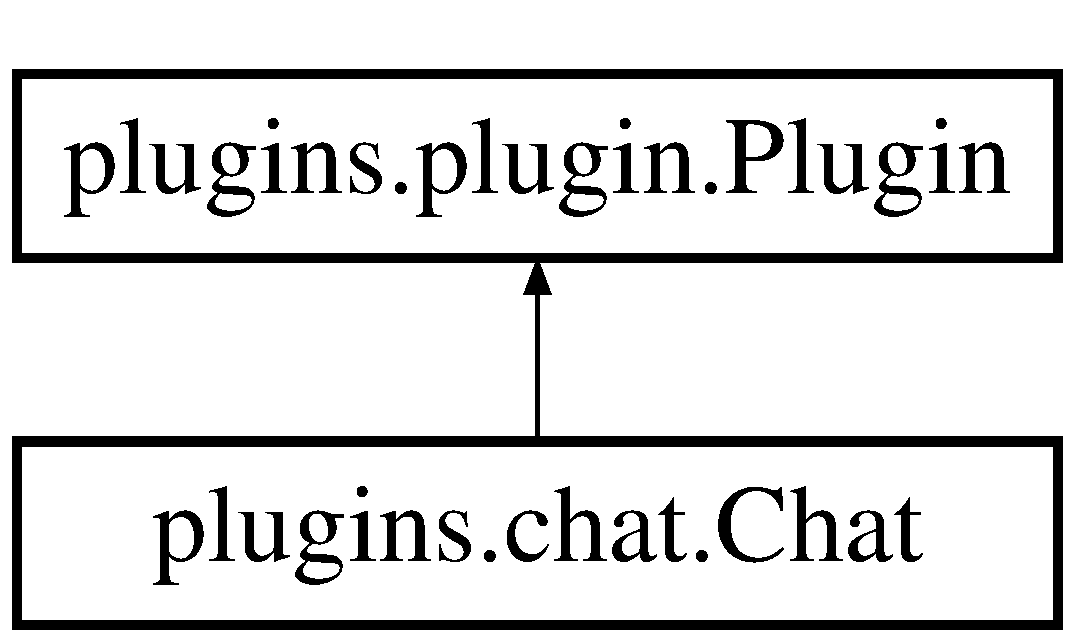
\includegraphics[height=2.000000cm]{classplugins_1_1chat_1_1_chat}
\end{center}
\end{figure}
\subsection*{\-Public \-Member \-Functions}
\begin{DoxyCompactItemize}
\item 
\hypertarget{classplugins_1_1chat_1_1_chat_ae62256183dbaeded5984584f1f324ab6}{def {\bfseries \-\_\-\-\_\-init\-\_\-\-\_\-}}\label{classplugins_1_1chat_1_1_chat_ae62256183dbaeded5984584f1f324ab6}

\item 
def \hyperlink{classplugins_1_1chat_1_1_chat_af8546a2537aee9bf99e09007649e2320}{server\-Message}
\item 
def \hyperlink{classplugins_1_1chat_1_1_chat_ad241689aeb8b03c689248ffb18584d40}{client\-Message}
\end{DoxyCompactItemize}
\subsection*{\-Public \-Attributes}
\begin{DoxyCompactItemize}
\item 
\hypertarget{classplugins_1_1chat_1_1_chat_a4082230dd09dc360fa943d7a491bc0b8}{{\bfseries msgs}}\label{classplugins_1_1chat_1_1_chat_a4082230dd09dc360fa943d7a491bc0b8}

\end{DoxyCompactItemize}
\subsection*{\-Static \-Public \-Attributes}
\begin{DoxyCompactItemize}
\item 
\hypertarget{classplugins_1_1chat_1_1_chat_ae47990387dbc71e4f121122c2c822aa8}{string {\bfseries \-M\-S\-G\-I\-D} = \char`\"{}chat\char`\"{}}\label{classplugins_1_1chat_1_1_chat_ae47990387dbc71e4f121122c2c822aa8}

\end{DoxyCompactItemize}


\subsection{\-Detailed \-Description}
\begin{DoxyVerb}Handles a minimalist chat plugin to be used in the game. \end{DoxyVerb}
 

\subsection{\-Member \-Function \-Documentation}
\hypertarget{classplugins_1_1chat_1_1_chat_ad241689aeb8b03c689248ffb18584d40}{\index{plugins\-::chat\-::\-Chat@{plugins\-::chat\-::\-Chat}!client\-Message@{client\-Message}}
\index{client\-Message@{client\-Message}!plugins::chat::Chat@{plugins\-::chat\-::\-Chat}}
\subsubsection[{client\-Message}]{\setlength{\rightskip}{0pt plus 5cm}def {\bf plugins.\-chat.\-Chat.\-client\-Message} (
\begin{DoxyParamCaption}
\item[{}]{self, }
\item[{}]{msg}
\end{DoxyParamCaption}
)}}\label{classplugins_1_1chat_1_1_chat_ad241689aeb8b03c689248ffb18584d40}
\begin{DoxyVerb}Receives a message and appends it to the messages to be displayed.
Then, it repaints the screen in order to update the view of the chat.
\end{DoxyVerb}
 

\-Reimplemented from \hyperlink{classplugins_1_1plugin_1_1_plugin_a9647791e5ba3150f5fd82bb359a43d11}{plugins.\-plugin.\-Plugin}.

\hypertarget{classplugins_1_1chat_1_1_chat_af8546a2537aee9bf99e09007649e2320}{\index{plugins\-::chat\-::\-Chat@{plugins\-::chat\-::\-Chat}!server\-Message@{server\-Message}}
\index{server\-Message@{server\-Message}!plugins::chat::Chat@{plugins\-::chat\-::\-Chat}}
\subsubsection[{server\-Message}]{\setlength{\rightskip}{0pt plus 5cm}def {\bf plugins.\-chat.\-Chat.\-server\-Message} (
\begin{DoxyParamCaption}
\item[{}]{self, }
\item[{}]{msg}
\end{DoxyParamCaption}
)}}\label{classplugins_1_1chat_1_1_chat_af8546a2537aee9bf99e09007649e2320}
\begin{DoxyVerb}Broadcasts a message on whole clients. \end{DoxyVerb}
 

\-Reimplemented from \hyperlink{classplugins_1_1plugin_1_1_plugin_aac06ba69452a3dac4e5950116a34d3ac}{plugins.\-plugin.\-Plugin}.



\-The documentation for this class was generated from the following file\-:\begin{DoxyCompactItemize}
\item 
src/plugins/chat.\-py\end{DoxyCompactItemize}

\hypertarget{classplugins_1_1chat_1_1_chat_u_i}{\section{plugins.\-chat.\-Chat\-U\-I \-Class \-Reference}
\label{classplugins_1_1chat_1_1_chat_u_i}\index{plugins.\-chat.\-Chat\-U\-I@{plugins.\-chat.\-Chat\-U\-I}}
}
\subsection*{\-Public \-Member \-Functions}
\begin{DoxyCompactItemize}
\item 
\hypertarget{classplugins_1_1chat_1_1_chat_u_i_a185f8f51e02a963b31b9b8927d973cab}{def {\bfseries \-\_\-\-\_\-init\-\_\-\-\_\-}}\label{classplugins_1_1chat_1_1_chat_u_i_a185f8f51e02a963b31b9b8927d973cab}

\item 
\hypertarget{classplugins_1_1chat_1_1_chat_u_i_a3214d4b0cb1ca2ecc14b9f20557831b5}{def {\bfseries reset}}\label{classplugins_1_1chat_1_1_chat_u_i_a3214d4b0cb1ca2ecc14b9f20557831b5}

\item 
def \hyperlink{classplugins_1_1chat_1_1_chat_u_i_a8ca26e03589001781eaf635977f8eed5}{handle\-Key}
\item 
\hypertarget{classplugins_1_1chat_1_1_chat_u_i_a6e95815ced02bbfce6bfec3964784368}{def {\bfseries draw}}\label{classplugins_1_1chat_1_1_chat_u_i_a6e95815ced02bbfce6bfec3964784368}

\end{DoxyCompactItemize}
\subsection*{\-Public \-Attributes}
\begin{DoxyCompactItemize}
\item 
\hypertarget{classplugins_1_1chat_1_1_chat_u_i_ae122f51127a1147db7778671275b0f63}{{\bfseries writing}}\label{classplugins_1_1chat_1_1_chat_u_i_ae122f51127a1147db7778671275b0f63}

\item 
\hypertarget{classplugins_1_1chat_1_1_chat_u_i_a96505c72247f990f688350d86f185b97}{{\bfseries text}}\label{classplugins_1_1chat_1_1_chat_u_i_a96505c72247f990f688350d86f185b97}

\end{DoxyCompactItemize}
\subsection*{\-Static \-Public \-Attributes}
\begin{DoxyCompactItemize}
\item 
\hypertarget{classplugins_1_1chat_1_1_chat_u_i_ac12aca5d062820d1de63548ecdb6d2d3}{int {\bfseries \-M\-I\-N\-W} = 1000}\label{classplugins_1_1chat_1_1_chat_u_i_ac12aca5d062820d1de63548ecdb6d2d3}

\item 
\hypertarget{classplugins_1_1chat_1_1_chat_u_i_a2ede898e1cc1f8589f3384b76ee7338b}{int {\bfseries \-M\-I\-N\-H} = 9}\label{classplugins_1_1chat_1_1_chat_u_i_a2ede898e1cc1f8589f3384b76ee7338b}

\item 
\hypertarget{classplugins_1_1chat_1_1_chat_u_i_a092da1fe3db5424ba5f288af20b8444c}{int {\bfseries \-X} = 0}\label{classplugins_1_1chat_1_1_chat_u_i_a092da1fe3db5424ba5f288af20b8444c}

\item 
\hypertarget{classplugins_1_1chat_1_1_chat_u_i_ab70f81172121c60d851b80db8caacb73}{{\bfseries \-Y} = -\/\-M\-I\-N\-H}\label{classplugins_1_1chat_1_1_chat_u_i_ab70f81172121c60d851b80db8caacb73}

\item 
\hypertarget{classplugins_1_1chat_1_1_chat_u_i_a442543339db2d7759a49c6c2cb333413}{string {\bfseries \-N\-A\-M\-E} = \char`\"{}\-Chat\char`\"{}}\label{classplugins_1_1chat_1_1_chat_u_i_a442543339db2d7759a49c6c2cb333413}

\item 
\hypertarget{classplugins_1_1chat_1_1_chat_u_i_a57ab855f20873a5dd369600af943d24e}{string {\bfseries \-H\-E\-L\-P} = \char`\"{}space \-: begin message\char`\"{}}\label{classplugins_1_1chat_1_1_chat_u_i_a57ab855f20873a5dd369600af943d24e}

\end{DoxyCompactItemize}


\subsection{\-Member \-Function \-Documentation}
\hypertarget{classplugins_1_1chat_1_1_chat_u_i_a8ca26e03589001781eaf635977f8eed5}{\index{plugins\-::chat\-::\-Chat\-U\-I@{plugins\-::chat\-::\-Chat\-U\-I}!handle\-Key@{handle\-Key}}
\index{handle\-Key@{handle\-Key}!plugins::chat::ChatUI@{plugins\-::chat\-::\-Chat\-U\-I}}
\subsubsection[{handle\-Key}]{\setlength{\rightskip}{0pt plus 5cm}def {\bf plugins.\-chat.\-Chat\-U\-I.\-handle\-Key} (
\begin{DoxyParamCaption}
\item[{}]{self, }
\item[{}]{key}
\end{DoxyParamCaption}
)}}\label{classplugins_1_1chat_1_1_chat_u_i_a8ca26e03589001781eaf635977f8eed5}
\begin{DoxyVerb}return True if the key has been used \end{DoxyVerb}
 

\-The documentation for this class was generated from the following file\-:\begin{DoxyCompactItemize}
\item 
src/plugins/chat.\-py\end{DoxyCompactItemize}

\hypertarget{classinterface_1_1chunk_1_1_chunk}{\section{interface.\-chunk.\-Chunk \-Class \-Reference}
\label{classinterface_1_1chunk_1_1_chunk}\index{interface.\-chunk.\-Chunk@{interface.\-chunk.\-Chunk}}
}
\subsection*{\-Public \-Member \-Functions}
\begin{DoxyCompactItemize}
\item 
\hypertarget{classinterface_1_1chunk_1_1_chunk_a11149d978c9f6ee9c7272214b1236869}{def {\bfseries \-\_\-\-\_\-init\-\_\-\-\_\-}}\label{classinterface_1_1chunk_1_1_chunk_a11149d978c9f6ee9c7272214b1236869}

\item 
\hypertarget{classinterface_1_1chunk_1_1_chunk_abc29661f82910e5678943674aa60dbd1}{def {\bfseries init\-\_\-chunk}}\label{classinterface_1_1chunk_1_1_chunk_abc29661f82910e5678943674aa60dbd1}

\item 
\hypertarget{classinterface_1_1chunk_1_1_chunk_abde5119452bf668f483c50b6e93333a6}{def {\bfseries render}}\label{classinterface_1_1chunk_1_1_chunk_abde5119452bf668f483c50b6e93333a6}

\item 
\hypertarget{classinterface_1_1chunk_1_1_chunk_af4ceacbb4669cc87800fd6da09f3db52}{def {\bfseries scale\-\_\-chunk}}\label{classinterface_1_1chunk_1_1_chunk_af4ceacbb4669cc87800fd6da09f3db52}

\item 
\hypertarget{classinterface_1_1chunk_1_1_chunk_ae5f9a88ac4e5a67765b854e288bdb317}{def {\bfseries update}}\label{classinterface_1_1chunk_1_1_chunk_ae5f9a88ac4e5a67765b854e288bdb317}

\item 
\hypertarget{classinterface_1_1chunk_1_1_chunk_ae81d602d31acce5d7c5e86d8116478dd}{def {\bfseries click\-\_\-trigger}}\label{classinterface_1_1chunk_1_1_chunk_ae81d602d31acce5d7c5e86d8116478dd}

\item 
\hypertarget{classinterface_1_1chunk_1_1_chunk_af0b2dfd6782de3a492eef961b370e59f}{def {\bfseries set\-\_\-state}}\label{classinterface_1_1chunk_1_1_chunk_af0b2dfd6782de3a492eef961b370e59f}

\item 
\hypertarget{classinterface_1_1chunk_1_1_chunk_a755d62925a041fcc6d7a50f5379e39ed}{def {\bfseries get\-\_\-state}}\label{classinterface_1_1chunk_1_1_chunk_a755d62925a041fcc6d7a50f5379e39ed}

\end{DoxyCompactItemize}
\subsection*{\-Public \-Attributes}
\begin{DoxyCompactItemize}
\item 
\hypertarget{classinterface_1_1chunk_1_1_chunk_a9e9cffbaf114b74359d253ff31c0c5cd}{{\bfseries index}}\label{classinterface_1_1chunk_1_1_chunk_a9e9cffbaf114b74359d253ff31c0c5cd}

\item 
\hypertarget{classinterface_1_1chunk_1_1_chunk_ab22d666887dd6a32553bf295f505898e}{{\bfseries cells}}\label{classinterface_1_1chunk_1_1_chunk_ab22d666887dd6a32553bf295f505898e}

\item 
\hypertarget{classinterface_1_1chunk_1_1_chunk_a6e51c90bc606e659cdd545a6480bba9b}{{\bfseries g\-\_\-width}}\label{classinterface_1_1chunk_1_1_chunk_a6e51c90bc606e659cdd545a6480bba9b}

\item 
\hypertarget{classinterface_1_1chunk_1_1_chunk_a8dfa9db057a4891e8d512c331b612beb}{{\bfseries g\-\_\-height}}\label{classinterface_1_1chunk_1_1_chunk_a8dfa9db057a4891e8d512c331b612beb}

\item 
\hypertarget{classinterface_1_1chunk_1_1_chunk_aa13bd571b7c17aed303a19ba25b70e5b}{{\bfseries g\-\_\-map\-\_\-height}}\label{classinterface_1_1chunk_1_1_chunk_aa13bd571b7c17aed303a19ba25b70e5b}

\item 
\hypertarget{classinterface_1_1chunk_1_1_chunk_ad2925dfd3abda7f6c167f3913a8eeff8}{{\bfseries width}}\label{classinterface_1_1chunk_1_1_chunk_ad2925dfd3abda7f6c167f3913a8eeff8}

\item 
\hypertarget{classinterface_1_1chunk_1_1_chunk_a1d4d24ee8fbdb41168bea37b7e65c96e}{{\bfseries height}}\label{classinterface_1_1chunk_1_1_chunk_a1d4d24ee8fbdb41168bea37b7e65c96e}

\item 
\hypertarget{classinterface_1_1chunk_1_1_chunk_aada33185627c42d8e2a8252c49bb4348}{{\bfseries pos}}\label{classinterface_1_1chunk_1_1_chunk_aada33185627c42d8e2a8252c49bb4348}

\item 
\hypertarget{classinterface_1_1chunk_1_1_chunk_a89aee4adb10ca0001e03913adcc63fac}{{\bfseries base\-\_\-rect}}\label{classinterface_1_1chunk_1_1_chunk_a89aee4adb10ca0001e03913adcc63fac}

\item 
\hypertarget{classinterface_1_1chunk_1_1_chunk_a573d05a8d856b9c36bb0998fd1c63b63}{{\bfseries layers}}\label{classinterface_1_1chunk_1_1_chunk_a573d05a8d856b9c36bb0998fd1c63b63}

\item 
\hypertarget{classinterface_1_1chunk_1_1_chunk_a6a32dbe5b3215dc8209d9cc0e213ddfb}{{\bfseries image}}\label{classinterface_1_1chunk_1_1_chunk_a6a32dbe5b3215dc8209d9cc0e213ddfb}

\end{DoxyCompactItemize}


\-The documentation for this class was generated from the following file\-:\begin{DoxyCompactItemize}
\item 
src/interface/chunk.\-py\end{DoxyCompactItemize}

\hypertarget{classinterface_1_1cache_1_1_chunk_cache}{\section{interface.\-cache.\-Chunk\-Cache \-Class \-Reference}
\label{classinterface_1_1cache_1_1_chunk_cache}\index{interface.\-cache.\-Chunk\-Cache@{interface.\-cache.\-Chunk\-Cache}}
}
\-Inheritance diagram for interface.\-cache.\-Chunk\-Cache\-:\begin{figure}[H]
\begin{center}
\leavevmode
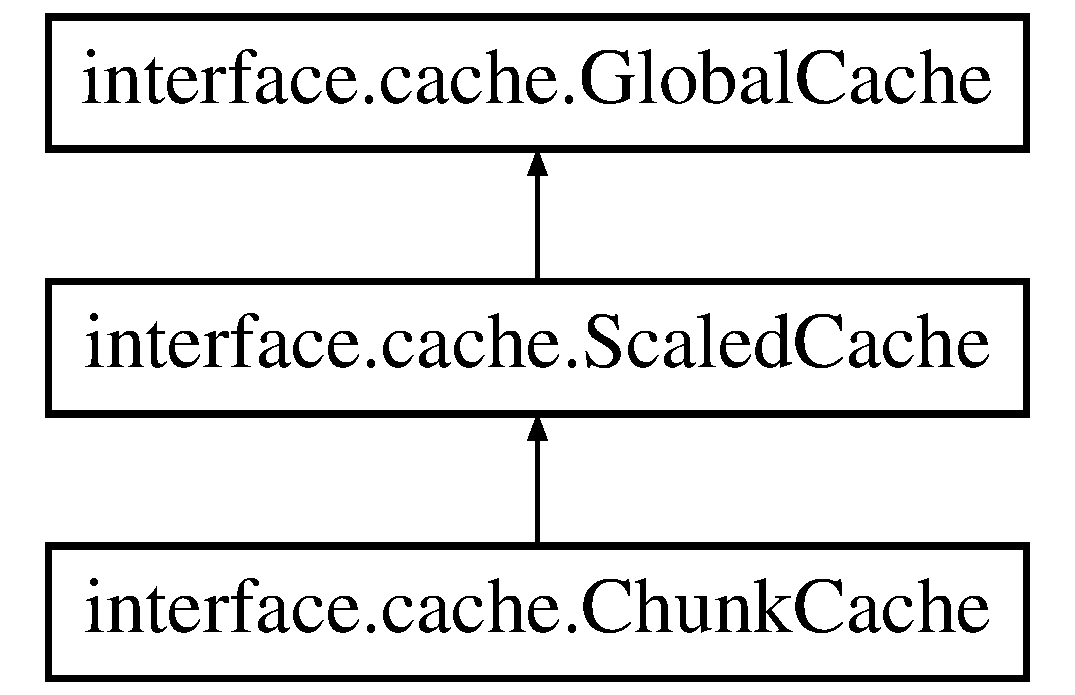
\includegraphics[height=3.000000cm]{classinterface_1_1cache_1_1_chunk_cache}
\end{center}
\end{figure}
\subsection*{\-Public \-Member \-Functions}
\begin{DoxyCompactItemize}
\item 
\hypertarget{classinterface_1_1cache_1_1_chunk_cache_a5ac68eaf44d3cac99bf98abfd39f687f}{def {\bfseries init\-\_\-chunk}}\label{classinterface_1_1cache_1_1_chunk_cache_a5ac68eaf44d3cac99bf98abfd39f687f}

\item 
\hypertarget{classinterface_1_1cache_1_1_chunk_cache_a7e1654f10929d2926638394c5ed1ebe4}{def {\bfseries init\-\_\-elts}}\label{classinterface_1_1cache_1_1_chunk_cache_a7e1654f10929d2926638394c5ed1ebe4}

\item 
\hypertarget{classinterface_1_1cache_1_1_chunk_cache_a7cc0a8f2a46b4cd1077d9f80d7c630d3}{def {\bfseries init\-\_\-chunks}}\label{classinterface_1_1cache_1_1_chunk_cache_a7cc0a8f2a46b4cd1077d9f80d7c630d3}

\item 
\hypertarget{classinterface_1_1cache_1_1_chunk_cache_af0c5eef3be5ec6bae095364e0abad836}{def {\bfseries get\-\_\-chunk}}\label{classinterface_1_1cache_1_1_chunk_cache_af0c5eef3be5ec6bae095364e0abad836}

\item 
\hypertarget{classinterface_1_1cache_1_1_chunk_cache_afa0d658ec0cfa2cc39cad48f265bdbe3}{def {\bfseries add\-\_\-scaled}}\label{classinterface_1_1cache_1_1_chunk_cache_afa0d658ec0cfa2cc39cad48f265bdbe3}

\end{DoxyCompactItemize}
\subsection*{\-Static \-Public \-Attributes}
\begin{DoxyCompactItemize}
\item 
\hypertarget{classinterface_1_1cache_1_1_chunk_cache_a5fc8e93b1ff937abe96a96a0dc99d4be}{dictionary {\bfseries cache} = \{\}}\label{classinterface_1_1cache_1_1_chunk_cache_a5fc8e93b1ff937abe96a96a0dc99d4be}

\end{DoxyCompactItemize}


\subsection{\-Detailed \-Description}
\begin{DoxyVerb}
Cache containing instanced chunks. Scale is used for the zoom while
playing the game.
\end{DoxyVerb}
 

\-The documentation for this class was generated from the following file\-:\begin{DoxyCompactItemize}
\item 
src/interface/cache.\-py\end{DoxyCompactItemize}

\hypertarget{classclient_1_1_client}{\section{client.\-Client \-Class \-Reference}
\label{classclient_1_1_client}\index{client.\-Client@{client.\-Client}}
}
\subsection*{\-Public \-Member \-Functions}
\begin{DoxyCompactItemize}
\item 
\hypertarget{classclient_1_1_client_a02d35b9c722c0434fda44d8b67274f8b}{def {\bfseries \-\_\-\-\_\-init\-\_\-\-\_\-}}\label{classclient_1_1_client_a02d35b9c722c0434fda44d8b67274f8b}

\item 
def \hyperlink{classclient_1_1_client_a81808356345d9f5b1c37200ce09a03cf}{\-\_\-\-\_\-del\-\_\-\-\_\-}
\item 
\hypertarget{classclient_1_1_client_a611a6aa5f1b60a60270b1cacc3522cb8}{def {\bfseries run}}\label{classclient_1_1_client_a611a6aa5f1b60a60270b1cacc3522cb8}

\item 
\hypertarget{classclient_1_1_client_aeff3316ccd3dc3efc6e216657ad11209}{def {\bfseries get\-Entity}}\label{classclient_1_1_client_aeff3316ccd3dc3efc6e216657ad11209}

\item 
\hypertarget{classclient_1_1_client_a29ca5ab810f2b176127fabe4a6e6e9f2}{def {\bfseries main}}\label{classclient_1_1_client_a29ca5ab810f2b176127fabe4a6e6e9f2}

\item 
\hypertarget{classclient_1_1_client_a411fe3cb0e6bd641925c600482025075}{def {\bfseries handle\-Order}}\label{classclient_1_1_client_a411fe3cb0e6bd641925c600482025075}

\item 
\hypertarget{classclient_1_1_client_ab33a0618c1e787648f00d5f36cb4fec8}{def {\bfseries plugin\-Handle}}\label{classclient_1_1_client_ab33a0618c1e787648f00d5f36cb4fec8}

\end{DoxyCompactItemize}
\subsection*{\-Public \-Attributes}
\begin{DoxyCompactItemize}
\item 
\hypertarget{classclient_1_1_client_a8cb5660eab73a84ffff78f931fba9f4a}{{\bfseries loop}}\label{classclient_1_1_client_a8cb5660eab73a84ffff78f931fba9f4a}

\item 
\hypertarget{classclient_1_1_client_a0bfd89eab5cd378c69d11a95ec3e9771}{{\bfseries net}}\label{classclient_1_1_client_a0bfd89eab5cd378c69d11a95ec3e9771}

\item 
\hypertarget{classclient_1_1_client_a514fa5a25b192d7c319dac3e81589139}{{\bfseries world}}\label{classclient_1_1_client_a514fa5a25b192d7c319dac3e81589139}

\item 
\hypertarget{classclient_1_1_client_a155c1a6cd1cd389f752946ae1be7df4e}{{\bfseries plugins}}\label{classclient_1_1_client_a155c1a6cd1cd389f752946ae1be7df4e}

\item 
\hypertarget{classclient_1_1_client_ac94a649fda29e1ef94a92729ce7c345c}{{\bfseries interface}}\label{classclient_1_1_client_ac94a649fda29e1ef94a92729ce7c345c}

\item 
\hypertarget{classclient_1_1_client_a2c24cff4ee58fef1de7de126cef3840e}{{\bfseries interactions}}\label{classclient_1_1_client_a2c24cff4ee58fef1de7de126cef3840e}

\item 
\hypertarget{classclient_1_1_client_a3f9927aadf41668bb2398b6404296076}{{\bfseries perso}}\label{classclient_1_1_client_a3f9927aadf41668bb2398b6404296076}

\item 
\hypertarget{classclient_1_1_client_a55b0a0b65f2cbc5bbeab157000db0ff4}{{\bfseries order\-Dispatcher}}\label{classclient_1_1_client_a55b0a0b65f2cbc5bbeab157000db0ff4}

\item 
\hypertarget{classclient_1_1_client_a80840f1460afc8548a654b36e7ca69f0}{{\bfseries net\-Task}}\label{classclient_1_1_client_a80840f1460afc8548a654b36e7ca69f0}

\end{DoxyCompactItemize}


\subsection{\-Detailed \-Description}
\begin{DoxyVerb}Main class of the client process, gathering interface, world and networking\end{DoxyVerb}
 

\subsection{\-Constructor \& \-Destructor \-Documentation}
\hypertarget{classclient_1_1_client_a81808356345d9f5b1c37200ce09a03cf}{\index{client\-::\-Client@{client\-::\-Client}!\-\_\-\-\_\-del\-\_\-\-\_\-@{\-\_\-\-\_\-del\-\_\-\-\_\-}}
\index{\-\_\-\-\_\-del\-\_\-\-\_\-@{\-\_\-\-\_\-del\-\_\-\-\_\-}!client::Client@{client\-::\-Client}}
\subsubsection[{\-\_\-\-\_\-del\-\_\-\-\_\-}]{\setlength{\rightskip}{0pt plus 5cm}def {\bf client.\-Client.\-\_\-\-\_\-del\-\_\-\-\_\-} (
\begin{DoxyParamCaption}
\item[{}]{self}
\end{DoxyParamCaption}
)}}\label{classclient_1_1_client_a81808356345d9f5b1c37200ce09a03cf}
\begin{DoxyVerb}Kill network and interface \end{DoxyVerb}
 

\-The documentation for this class was generated from the following file\-:\begin{DoxyCompactItemize}
\item 
src/client.\-py\end{DoxyCompactItemize}

\hypertarget{classinterface_1_1pygamecli_1_1_client}{\section{interface.\-pygamecli.\-Client \-Class \-Reference}
\label{classinterface_1_1pygamecli_1_1_client}\index{interface.\-pygamecli.\-Client@{interface.\-pygamecli.\-Client}}
}
\-Inheritance diagram for interface.\-pygamecli.\-Client\-:\begin{figure}[H]
\begin{center}
\leavevmode
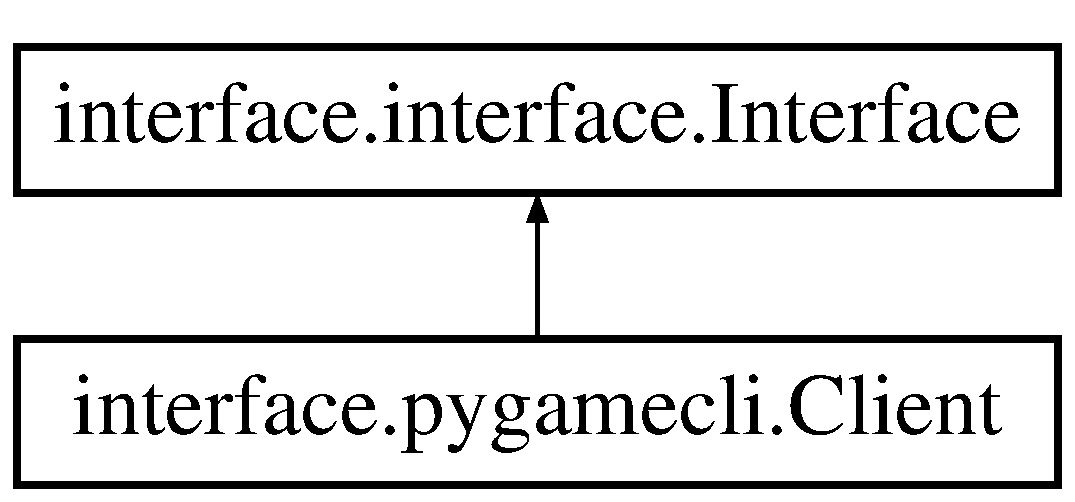
\includegraphics[height=2.000000cm]{classinterface_1_1pygamecli_1_1_client}
\end{center}
\end{figure}
\subsection*{\-Public \-Member \-Functions}
\begin{DoxyCompactItemize}
\item 
\hypertarget{classinterface_1_1pygamecli_1_1_client_a4472ac4b9b9fdf3f3ffa823cc0ec802d}{def {\bfseries \-\_\-\-\_\-init\-\_\-\-\_\-}}\label{classinterface_1_1pygamecli_1_1_client_a4472ac4b9b9fdf3f3ffa823cc0ec802d}

\item 
\hypertarget{classinterface_1_1pygamecli_1_1_client_ac80a9a1d9f3baa16bd52eed1875ec1e9}{def {\bfseries \-\_\-\-\_\-del\-\_\-\-\_\-}}\label{classinterface_1_1pygamecli_1_1_client_ac80a9a1d9f3baa16bd52eed1875ec1e9}

\item 
\hypertarget{classinterface_1_1pygamecli_1_1_client_ae958c1468bdab4c66913bb54bdb7cf9f}{def {\bfseries get\-Event}}\label{classinterface_1_1pygamecli_1_1_client_ae958c1468bdab4c66913bb54bdb7cf9f}

\item 
\hypertarget{classinterface_1_1pygamecli_1_1_client_a9b6826bca386c136ab018ed86371fd18}{def {\bfseries set\-\_\-perso}}\label{classinterface_1_1pygamecli_1_1_client_a9b6826bca386c136ab018ed86371fd18}

\item 
\hypertarget{classinterface_1_1pygamecli_1_1_client_af359e0ff9462666fad74f25339b47f89}{def {\bfseries init}}\label{classinterface_1_1pygamecli_1_1_client_af359e0ff9462666fad74f25339b47f89}

\item 
\hypertarget{classinterface_1_1pygamecli_1_1_client_a09519388ef07cdfc01ff6fc2b127aa86}{def {\bfseries update}}\label{classinterface_1_1pygamecli_1_1_client_a09519388ef07cdfc01ff6fc2b127aa86}

\item 
\hypertarget{classinterface_1_1pygamecli_1_1_client_a50fac3d1fced530d373c7ea9bd8d37c3}{def {\bfseries frame\-\_\-counter}}\label{classinterface_1_1pygamecli_1_1_client_a50fac3d1fced530d373c7ea9bd8d37c3}

\item 
\hypertarget{classinterface_1_1pygamecli_1_1_client_ab35e5031ac58f6ea79e221da713e6e80}{def {\bfseries update\-\_\-view}}\label{classinterface_1_1pygamecli_1_1_client_ab35e5031ac58f6ea79e221da713e6e80}

\item 
\hypertarget{classinterface_1_1pygamecli_1_1_client_a4450a249f1987b7b86db64655d36b256}{def {\bfseries get\-\_\-conf\-\_\-file}}\label{classinterface_1_1pygamecli_1_1_client_a4450a249f1987b7b86db64655d36b256}

\item 
\hypertarget{classinterface_1_1pygamecli_1_1_client_a30a6ed85525dfb19a958e0b464055c7e}{def {\bfseries get\-\_\-conf}}\label{classinterface_1_1pygamecli_1_1_client_a30a6ed85525dfb19a958e0b464055c7e}

\item 
\hypertarget{classinterface_1_1pygamecli_1_1_client_aa38313ece4d971180386cdb5ffccd5eb}{def {\bfseries init\-\_\-cache}}\label{classinterface_1_1pygamecli_1_1_client_aa38313ece4d971180386cdb5ffccd5eb}

\item 
\hypertarget{classinterface_1_1pygamecli_1_1_client_a72aa59586338a4fa2d64b24c1f57ba77}{def {\bfseries handle\-Order}}\label{classinterface_1_1pygamecli_1_1_client_a72aa59586338a4fa2d64b24c1f57ba77}

\end{DoxyCompactItemize}
\subsection*{\-Public \-Attributes}
\begin{DoxyCompactItemize}
\item 
\hypertarget{classinterface_1_1pygamecli_1_1_client_a5118a5cf2209a04a63371b75315cb84f}{{\bfseries screen\-\_\-size}}\label{classinterface_1_1pygamecli_1_1_client_a5118a5cf2209a04a63371b75315cb84f}

\item 
\hypertarget{classinterface_1_1pygamecli_1_1_client_a21ee5fde2fbd01229b07471bfc7d1959}{{\bfseries screen}}\label{classinterface_1_1pygamecli_1_1_client_a21ee5fde2fbd01229b07471bfc7d1959}

\item 
\hypertarget{classinterface_1_1pygamecli_1_1_client_aa9382f8985478be4880bbc3eff6f40ac}{{\bfseries world}}\label{classinterface_1_1pygamecli_1_1_client_aa9382f8985478be4880bbc3eff6f40ac}

\item 
\hypertarget{classinterface_1_1pygamecli_1_1_client_ad01a7f015a217313424028f3c4049b47}{{\bfseries interface}}\label{classinterface_1_1pygamecli_1_1_client_ad01a7f015a217313424028f3c4049b47}

\item 
\hypertarget{classinterface_1_1pygamecli_1_1_client_a5c60ef342da839d2673dab28edb67b33}{{\bfseries perso}}\label{classinterface_1_1pygamecli_1_1_client_a5c60ef342da839d2673dab28edb67b33}

\item 
\hypertarget{classinterface_1_1pygamecli_1_1_client_a7c32edb978943050ffa68740426c3683}{{\bfseries font}}\label{classinterface_1_1pygamecli_1_1_client_a7c32edb978943050ffa68740426c3683}

\item 
\hypertarget{classinterface_1_1pygamecli_1_1_client_aebcb27b71a1bc083c763850efef433e0}{{\bfseries background}}\label{classinterface_1_1pygamecli_1_1_client_aebcb27b71a1bc083c763850efef433e0}

\item 
\hypertarget{classinterface_1_1pygamecli_1_1_client_abb6bf425334783e24b4b9ec04ef05cbb}{{\bfseries clock}}\label{classinterface_1_1pygamecli_1_1_client_abb6bf425334783e24b4b9ec04ef05cbb}

\item 
\hypertarget{classinterface_1_1pygamecli_1_1_client_aa59c8ed1b463a472c3200db5910ba2ec}{{\bfseries mov\-\_\-speed\-\_\-x}}\label{classinterface_1_1pygamecli_1_1_client_aa59c8ed1b463a472c3200db5910ba2ec}

\item 
\hypertarget{classinterface_1_1pygamecli_1_1_client_a5873c97fb0648bd1326ca1b0c7358847}{{\bfseries mov\-\_\-speed\-\_\-y}}\label{classinterface_1_1pygamecli_1_1_client_a5873c97fb0648bd1326ca1b0c7358847}

\item 
\hypertarget{classinterface_1_1pygamecli_1_1_client_a3ffb39f9ae93cfae520080286d2d813d}{{\bfseries refresh\-\_\-counter}}\label{classinterface_1_1pygamecli_1_1_client_a3ffb39f9ae93cfae520080286d2d813d}

\item 
\hypertarget{classinterface_1_1pygamecli_1_1_client_a630ff935559ffad8d89d31cc96ebca72}{{\bfseries conf}}\label{classinterface_1_1pygamecli_1_1_client_a630ff935559ffad8d89d31cc96ebca72}

\end{DoxyCompactItemize}


\-The documentation for this class was generated from the following file\-:\begin{DoxyCompactItemize}
\item 
src/interface/pygamecli.\-py\end{DoxyCompactItemize}

\hypertarget{classinterface_1_1cursescli_1_1_curses}{\section{interface.\-cursescli.\-Curses \-Class \-Reference}
\label{classinterface_1_1cursescli_1_1_curses}\index{interface.\-cursescli.\-Curses@{interface.\-cursescli.\-Curses}}
}
\-Inheritance diagram for interface.\-cursescli.\-Curses\-:\begin{figure}[H]
\begin{center}
\leavevmode
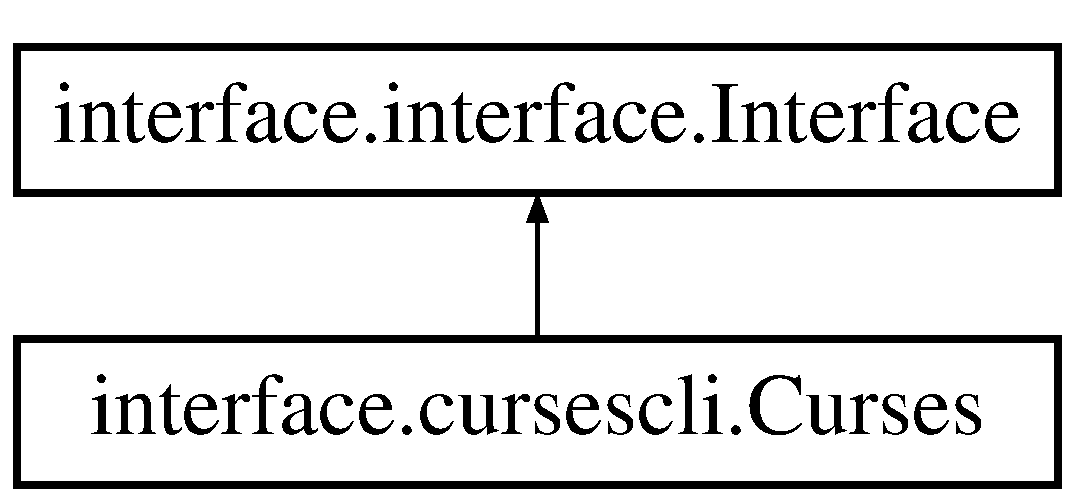
\includegraphics[height=2.000000cm]{classinterface_1_1cursescli_1_1_curses}
\end{center}
\end{figure}
\subsection*{\-Public \-Member \-Functions}
\begin{DoxyCompactItemize}
\item 
\hypertarget{classinterface_1_1cursescli_1_1_curses_a192eb6300c83226e1b98e4d7a5bc9561}{def {\bfseries \-\_\-\-\_\-init\-\_\-\-\_\-}}\label{classinterface_1_1cursescli_1_1_curses_a192eb6300c83226e1b98e4d7a5bc9561}

\item 
def \hyperlink{classinterface_1_1cursescli_1_1_curses_ab2b4383b3add0916dfce994865013c12}{resize}
\item 
\hypertarget{classinterface_1_1cursescli_1_1_curses_a6ab69ed1b7afdc9d1d0f7e74ed6623cd}{def {\bfseries init}}\label{classinterface_1_1cursescli_1_1_curses_a6ab69ed1b7afdc9d1d0f7e74ed6623cd}

\item 
\hypertarget{classinterface_1_1cursescli_1_1_curses_a003586d92839ef7c13b164829e5ea5a4}{def {\bfseries set\-Perso}}\label{classinterface_1_1cursescli_1_1_curses_a003586d92839ef7c13b164829e5ea5a4}

\item 
\hypertarget{classinterface_1_1cursescli_1_1_curses_a03c24991bdaf625425fcdc00a31dd880}{def {\bfseries repaint}}\label{classinterface_1_1cursescli_1_1_curses_a03c24991bdaf625425fcdc00a31dd880}

\item 
\hypertarget{classinterface_1_1cursescli_1_1_curses_ae94215f68f2e77264bcd8b2338cd9bd6}{def {\bfseries end}}\label{classinterface_1_1cursescli_1_1_curses_ae94215f68f2e77264bcd8b2338cd9bd6}

\item 
\hypertarget{classinterface_1_1cursescli_1_1_curses_a80b940406bbf923b5deff0fe6c35f4d4}{def {\bfseries get\-Event}}\label{classinterface_1_1cursescli_1_1_curses_a80b940406bbf923b5deff0fe6c35f4d4}

\end{DoxyCompactItemize}
\subsection*{\-Public \-Attributes}
\begin{DoxyCompactItemize}
\item 
\hypertarget{classinterface_1_1cursescli_1_1_curses_aef928128c6047b9f58b5563951b368c7}{{\bfseries win}}\label{classinterface_1_1cursescli_1_1_curses_aef928128c6047b9f58b5563951b368c7}

\item 
\hypertarget{classinterface_1_1cursescli_1_1_curses_a3489b03044b2c13a4db2ea5ed887b0b3}{{\bfseries map\-View}}\label{classinterface_1_1cursescli_1_1_curses_a3489b03044b2c13a4db2ea5ed887b0b3}

\item 
\hypertarget{classinterface_1_1cursescli_1_1_curses_a129e60c1720fbd8041b15d2d54dcbb74}{{\bfseries to\-Small}}\label{classinterface_1_1cursescli_1_1_curses_a129e60c1720fbd8041b15d2d54dcbb74}

\end{DoxyCompactItemize}


\subsection{\-Detailed \-Description}
\begin{DoxyVerb}ncurses-based UI \end{DoxyVerb}
 

\subsection{\-Member \-Function \-Documentation}
\hypertarget{classinterface_1_1cursescli_1_1_curses_ab2b4383b3add0916dfce994865013c12}{\index{interface\-::cursescli\-::\-Curses@{interface\-::cursescli\-::\-Curses}!resize@{resize}}
\index{resize@{resize}!interface::cursescli::Curses@{interface\-::cursescli\-::\-Curses}}
\subsubsection[{resize}]{\setlength{\rightskip}{0pt plus 5cm}def {\bf interface.\-cursescli.\-Curses.\-resize} (
\begin{DoxyParamCaption}
\item[{}]{self}
\end{DoxyParamCaption}
)}}\label{classinterface_1_1cursescli_1_1_curses_ab2b4383b3add0916dfce994865013c12}
\begin{DoxyVerb}Computes plugins positions \end{DoxyVerb}
 

\-The documentation for this class was generated from the following file\-:\begin{DoxyCompactItemize}
\item 
src/interface/cursescli.\-py\end{DoxyCompactItemize}

\hypertarget{classplugins_1_1plugin_1_1_curses_plugin}{\section{plugins.\-plugin.\-Curses\-Plugin \-Class \-Reference}
\label{classplugins_1_1plugin_1_1_curses_plugin}\index{plugins.\-plugin.\-Curses\-Plugin@{plugins.\-plugin.\-Curses\-Plugin}}
}
\-Inheritance diagram for plugins.\-plugin.\-Curses\-Plugin\-:\begin{figure}[H]
\begin{center}
\leavevmode
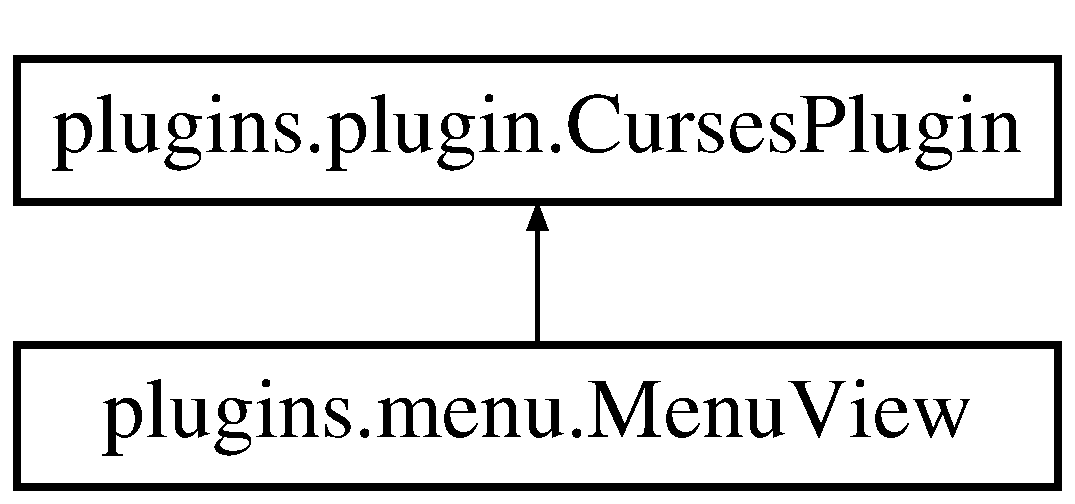
\includegraphics[height=2.000000cm]{classplugins_1_1plugin_1_1_curses_plugin}
\end{center}
\end{figure}
\subsection*{\-Public \-Member \-Functions}
\begin{DoxyCompactItemize}
\item 
\hypertarget{classplugins_1_1plugin_1_1_curses_plugin_a7dfd26b80b3427f79337e100053dca74}{def {\bfseries \-\_\-\-\_\-init\-\_\-\-\_\-}}\label{classplugins_1_1plugin_1_1_curses_plugin_a7dfd26b80b3427f79337e100053dca74}

\item 
def \hyperlink{classplugins_1_1plugin_1_1_curses_plugin_a4c40f3646ac95d9dc1e03f92ee1f7491}{handle\-Key}
\item 
def \hyperlink{classplugins_1_1plugin_1_1_curses_plugin_ae9cdc9674d47a60ce7e44c367a8c1404}{draw}
\item 
\hypertarget{classplugins_1_1plugin_1_1_curses_plugin_a4a0aa93ca4d0c63914646f8bf8b8f002}{def {\bfseries repaint}}\label{classplugins_1_1plugin_1_1_curses_plugin_a4a0aa93ca4d0c63914646f8bf8b8f002}

\end{DoxyCompactItemize}
\subsection*{\-Public \-Attributes}
\begin{DoxyCompactItemize}
\item 
\hypertarget{classplugins_1_1plugin_1_1_curses_plugin_a3103a9de7bd546901cc8d7a3dce0ab21}{{\bfseries win}}\label{classplugins_1_1plugin_1_1_curses_plugin_a3103a9de7bd546901cc8d7a3dce0ab21}

\item 
\hypertarget{classplugins_1_1plugin_1_1_curses_plugin_a4ef84b72273f12712ff36b7b6a2c5b58}{{\bfseries net\-Plugin}}\label{classplugins_1_1plugin_1_1_curses_plugin_a4ef84b72273f12712ff36b7b6a2c5b58}

\item 
\hypertarget{classplugins_1_1plugin_1_1_curses_plugin_a12b63d1fbcd2c3da0a8175a7bf5fda47}{{\bfseries interface}}\label{classplugins_1_1plugin_1_1_curses_plugin_a12b63d1fbcd2c3da0a8175a7bf5fda47}

\item 
\hypertarget{classplugins_1_1plugin_1_1_curses_plugin_a776b6d2b58afa9f4fa0ac78c954d7a8e}{{\bfseries width}}\label{classplugins_1_1plugin_1_1_curses_plugin_a776b6d2b58afa9f4fa0ac78c954d7a8e}

\end{DoxyCompactItemize}
\subsection*{\-Static \-Public \-Attributes}
\begin{DoxyCompactItemize}
\item 
\hypertarget{classplugins_1_1plugin_1_1_curses_plugin_a96e814f68492e1cebbc7f958dac39b18}{int {\bfseries \-M\-I\-N\-W} = 0}\label{classplugins_1_1plugin_1_1_curses_plugin_a96e814f68492e1cebbc7f958dac39b18}

\item 
\hypertarget{classplugins_1_1plugin_1_1_curses_plugin_a1a544956a9b29a11e9b939204a19dd11}{int {\bfseries \-M\-I\-N\-H} = 0}\label{classplugins_1_1plugin_1_1_curses_plugin_a1a544956a9b29a11e9b939204a19dd11}

\item 
\hypertarget{classplugins_1_1plugin_1_1_curses_plugin_a8281f47102eff4b69a42b082bbf2f649}{string {\bfseries \-N\-A\-M\-E} = \char`\"{}\char`\"{}}\label{classplugins_1_1plugin_1_1_curses_plugin_a8281f47102eff4b69a42b082bbf2f649}

\item 
\hypertarget{classplugins_1_1plugin_1_1_curses_plugin_ae01c2507e4c26e606768979d40036b5c}{tuple {\bfseries \-H\-E\-L\-P} = ()}\label{classplugins_1_1plugin_1_1_curses_plugin_ae01c2507e4c26e606768979d40036b5c}

\end{DoxyCompactItemize}


\subsection{\-Detailed \-Description}
\begin{DoxyVerb}Subclass this to write a curse plugin, appearing as a window.
MINW and MINH are the asked size and X,Y the placement that can be
negative to be on the other side.
Fill NAME and HELP to have an entry in the menu. \end{DoxyVerb}
 

\subsection{\-Member \-Function \-Documentation}
\hypertarget{classplugins_1_1plugin_1_1_curses_plugin_ae9cdc9674d47a60ce7e44c367a8c1404}{\index{plugins\-::plugin\-::\-Curses\-Plugin@{plugins\-::plugin\-::\-Curses\-Plugin}!draw@{draw}}
\index{draw@{draw}!plugins::plugin::CursesPlugin@{plugins\-::plugin\-::\-Curses\-Plugin}}
\subsubsection[{draw}]{\setlength{\rightskip}{0pt plus 5cm}def {\bf plugins.\-plugin.\-Curses\-Plugin.\-draw} (
\begin{DoxyParamCaption}
\item[{}]{self}
\end{DoxyParamCaption}
)}}\label{classplugins_1_1plugin_1_1_curses_plugin_ae9cdc9674d47a60ce7e44c367a8c1404}
\begin{DoxyVerb}don't forget to call self.win.noutrefresh after some changes \end{DoxyVerb}
 

\-Reimplemented in \hyperlink{classplugins_1_1menu_1_1_menu_view_a693bc4021b2a04bd22ceb15dde01a330}{plugins.\-menu.\-Menu\-View}.

\hypertarget{classplugins_1_1plugin_1_1_curses_plugin_a4c40f3646ac95d9dc1e03f92ee1f7491}{\index{plugins\-::plugin\-::\-Curses\-Plugin@{plugins\-::plugin\-::\-Curses\-Plugin}!handle\-Key@{handle\-Key}}
\index{handle\-Key@{handle\-Key}!plugins::plugin::CursesPlugin@{plugins\-::plugin\-::\-Curses\-Plugin}}
\subsubsection[{handle\-Key}]{\setlength{\rightskip}{0pt plus 5cm}def {\bf plugins.\-plugin.\-Curses\-Plugin.\-handle\-Key} (
\begin{DoxyParamCaption}
\item[{}]{self, }
\item[{}]{key}
\end{DoxyParamCaption}
)}}\label{classplugins_1_1plugin_1_1_curses_plugin_a4c40f3646ac95d9dc1e03f92ee1f7491}
\begin{DoxyVerb}return True if the key has been used \end{DoxyVerb}
 

\-The documentation for this class was generated from the following file\-:\begin{DoxyCompactItemize}
\item 
src/plugins/plugin.\-py\end{DoxyCompactItemize}

\hypertarget{classworld_1_1_entity}{\section{world.\-Entity \-Class \-Reference}
\label{classworld_1_1_entity}\index{world.\-Entity@{world.\-Entity}}
}
\-Inheritance diagram for world.\-Entity\-:\begin{figure}[H]
\begin{center}
\leavevmode
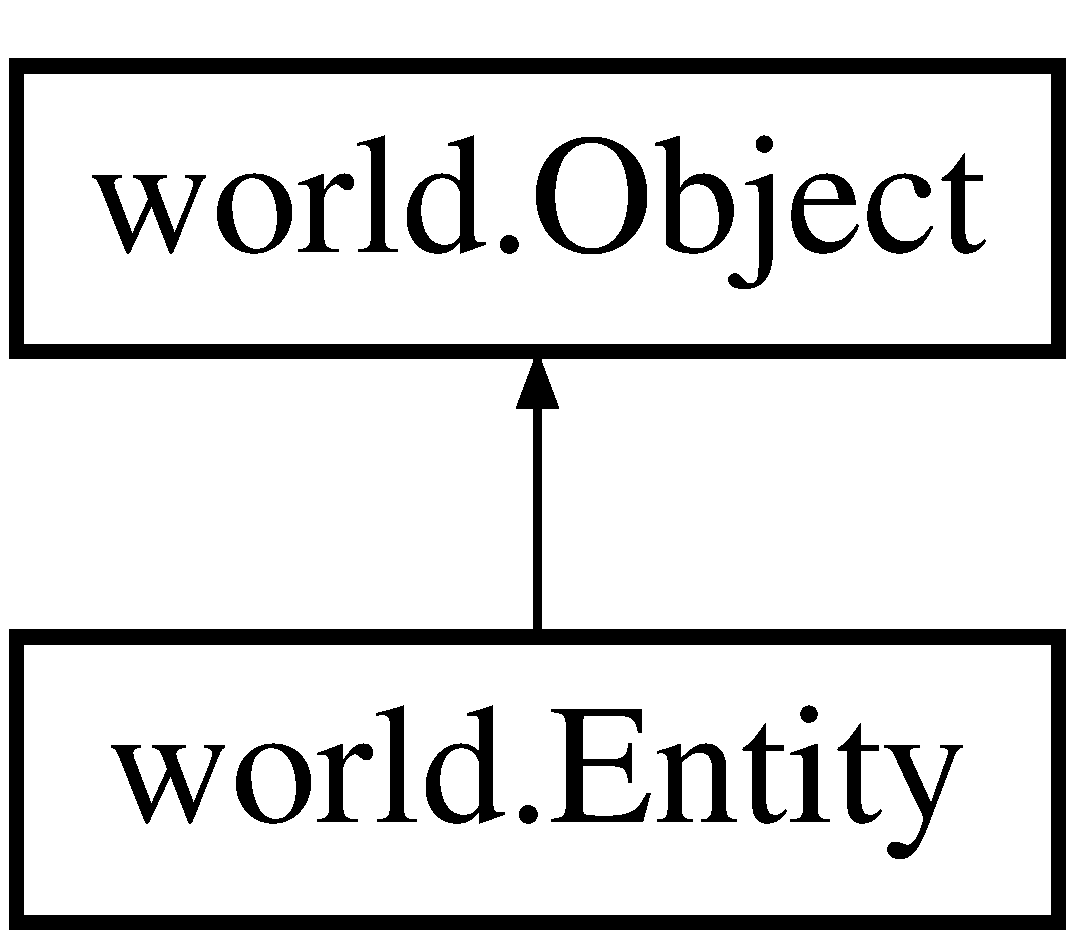
\includegraphics[height=2.000000cm]{classworld_1_1_entity}
\end{center}
\end{figure}
\subsection*{\-Public \-Member \-Functions}
\begin{DoxyCompactItemize}
\item 
\hypertarget{classworld_1_1_entity_ae3f6c9349b4756df29e482ae07582ca4}{def {\bfseries \-\_\-\-\_\-init\-\_\-\-\_\-}}\label{classworld_1_1_entity_ae3f6c9349b4756df29e482ae07582ca4}

\end{DoxyCompactItemize}
\subsection*{\-Public \-Attributes}
\begin{DoxyCompactItemize}
\item 
\hypertarget{classworld_1_1_entity_a02ac854a6a124cc8bfdef46ae7941434}{{\bfseries quests}}\label{classworld_1_1_entity_a02ac854a6a124cc8bfdef46ae7941434}

\item 
\hypertarget{classworld_1_1_entity_add2bc9bb2f731cc86228d8932a962e60}{{\bfseries inventory}}\label{classworld_1_1_entity_add2bc9bb2f731cc86228d8932a962e60}

\item 
\hypertarget{classworld_1_1_entity_a2e893d9acd136fa158874582882a3f13}{{\bfseries user}}\label{classworld_1_1_entity_a2e893d9acd136fa158874582882a3f13}

\end{DoxyCompactItemize}


\-The documentation for this class was generated from the following file\-:\begin{DoxyCompactItemize}
\item 
src/shared/world.\-py\end{DoxyCompactItemize}

\hypertarget{classinterface_1_1entity_1_1_entity}{\section{interface.\-entity.\-Entity \-Class \-Reference}
\label{classinterface_1_1entity_1_1_entity}\index{interface.\-entity.\-Entity@{interface.\-entity.\-Entity}}
}
\subsection*{\-Public \-Member \-Functions}
\begin{DoxyCompactItemize}
\item 
\hypertarget{classinterface_1_1entity_1_1_entity_a2d0ffe60ca9b28c2e3f60676d1571798}{def {\bfseries \-\_\-\-\_\-init\-\_\-\-\_\-}}\label{classinterface_1_1entity_1_1_entity_a2d0ffe60ca9b28c2e3f60676d1571798}

\item 
\hypertarget{classinterface_1_1entity_1_1_entity_a3711185e5f592a7a4a8ba43f68ea14e8}{def {\bfseries render}}\label{classinterface_1_1entity_1_1_entity_a3711185e5f592a7a4a8ba43f68ea14e8}

\item 
\hypertarget{classinterface_1_1entity_1_1_entity_acfef12dffdda93eae47da3fab5a3801d}{def {\bfseries get\-\_\-ent\-\_\-pos}}\label{classinterface_1_1entity_1_1_entity_acfef12dffdda93eae47da3fab5a3801d}

\item 
\hypertarget{classinterface_1_1entity_1_1_entity_a29f5969b06f3869feee65999f3af780d}{def {\bfseries update}}\label{classinterface_1_1entity_1_1_entity_a29f5969b06f3869feee65999f3af780d}

\end{DoxyCompactItemize}
\subsection*{\-Public \-Attributes}
\begin{DoxyCompactItemize}
\item 
\hypertarget{classinterface_1_1entity_1_1_entity_ae988add8b50095849685c1728b664983}{{\bfseries y}}\label{classinterface_1_1entity_1_1_entity_ae988add8b50095849685c1728b664983}

\item 
\hypertarget{classinterface_1_1entity_1_1_entity_a39d69517b193fbd597dd9e110fe72485}{{\bfseries map\-\_\-height}}\label{classinterface_1_1entity_1_1_entity_a39d69517b193fbd597dd9e110fe72485}

\item 
\hypertarget{classinterface_1_1entity_1_1_entity_a785b8e2968a9e83c39a3d12d27fb5b33}{{\bfseries picture}}\label{classinterface_1_1entity_1_1_entity_a785b8e2968a9e83c39a3d12d27fb5b33}

\item 
\hypertarget{classinterface_1_1entity_1_1_entity_ae9d2a77436bf20c3d52998f7e0f32e7d}{{\bfseries image}}\label{classinterface_1_1entity_1_1_entity_ae9d2a77436bf20c3d52998f7e0f32e7d}

\item 
\hypertarget{classinterface_1_1entity_1_1_entity_a692ddb28faef49c722bf8093c9113a58}{{\bfseries pos}}\label{classinterface_1_1entity_1_1_entity_a692ddb28faef49c722bf8093c9113a58}

\end{DoxyCompactItemize}


\-The documentation for this class was generated from the following file\-:\begin{DoxyCompactItemize}
\item 
src/interface/entity.\-py\end{DoxyCompactItemize}

\hypertarget{classinterface_1_1cache_1_1_global_cache}{\section{interface.\-cache.\-Global\-Cache \-Class \-Reference}
\label{classinterface_1_1cache_1_1_global_cache}\index{interface.\-cache.\-Global\-Cache@{interface.\-cache.\-Global\-Cache}}
}
\-Inheritance diagram for interface.\-cache.\-Global\-Cache\-:\begin{figure}[H]
\begin{center}
\leavevmode
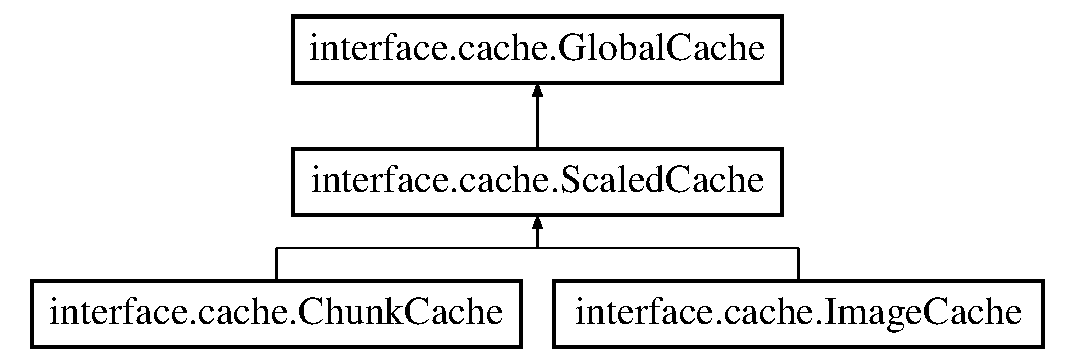
\includegraphics[height=3.000000cm]{classinterface_1_1cache_1_1_global_cache}
\end{center}
\end{figure}
\subsection*{\-Public \-Member \-Functions}
\begin{DoxyCompactItemize}
\item 
\hypertarget{classinterface_1_1cache_1_1_global_cache_a34b268830f3cfa197ec340c5460ceab7}{def {\bfseries \-\_\-\-\_\-init\-\_\-\-\_\-}}\label{classinterface_1_1cache_1_1_global_cache_a34b268830f3cfa197ec340c5460ceab7}

\item 
\hypertarget{classinterface_1_1cache_1_1_global_cache_ae65c7d3b274367f88bc8d8c0a72b931c}{def {\bfseries set}}\label{classinterface_1_1cache_1_1_global_cache_ae65c7d3b274367f88bc8d8c0a72b931c}

\item 
\hypertarget{classinterface_1_1cache_1_1_global_cache_ac8877671057ced93272ebe1e84d868f8}{def {\bfseries get}}\label{classinterface_1_1cache_1_1_global_cache_ac8877671057ced93272ebe1e84d868f8}

\item 
\hypertarget{classinterface_1_1cache_1_1_global_cache_ab01004f7ec7e95b4b06603a9634e836d}{def {\bfseries clear}}\label{classinterface_1_1cache_1_1_global_cache_ab01004f7ec7e95b4b06603a9634e836d}

\item 
\hypertarget{classinterface_1_1cache_1_1_global_cache_a604c489301634d518b3b38110a7c5ab9}{def {\bfseries keys}}\label{classinterface_1_1cache_1_1_global_cache_a604c489301634d518b3b38110a7c5ab9}

\item 
\hypertarget{classinterface_1_1cache_1_1_global_cache_a2ed92f5e3689115f4b75c605783ba6ee}{def {\bfseries show}}\label{classinterface_1_1cache_1_1_global_cache_a2ed92f5e3689115f4b75c605783ba6ee}

\end{DoxyCompactItemize}


\subsection{\-Detailed \-Description}
\begin{DoxyVerb}
A generic cache (key, value) association for objects.
\end{DoxyVerb}
 

\-The documentation for this class was generated from the following file\-:\begin{DoxyCompactItemize}
\item 
src/interface/cache.\-py\end{DoxyCompactItemize}

\hypertarget{classinterface_1_1cache_1_1_image_cache}{\section{interface.\-cache.\-Image\-Cache \-Class \-Reference}
\label{classinterface_1_1cache_1_1_image_cache}\index{interface.\-cache.\-Image\-Cache@{interface.\-cache.\-Image\-Cache}}
}
\-Inheritance diagram for interface.\-cache.\-Image\-Cache\-:\begin{figure}[H]
\begin{center}
\leavevmode
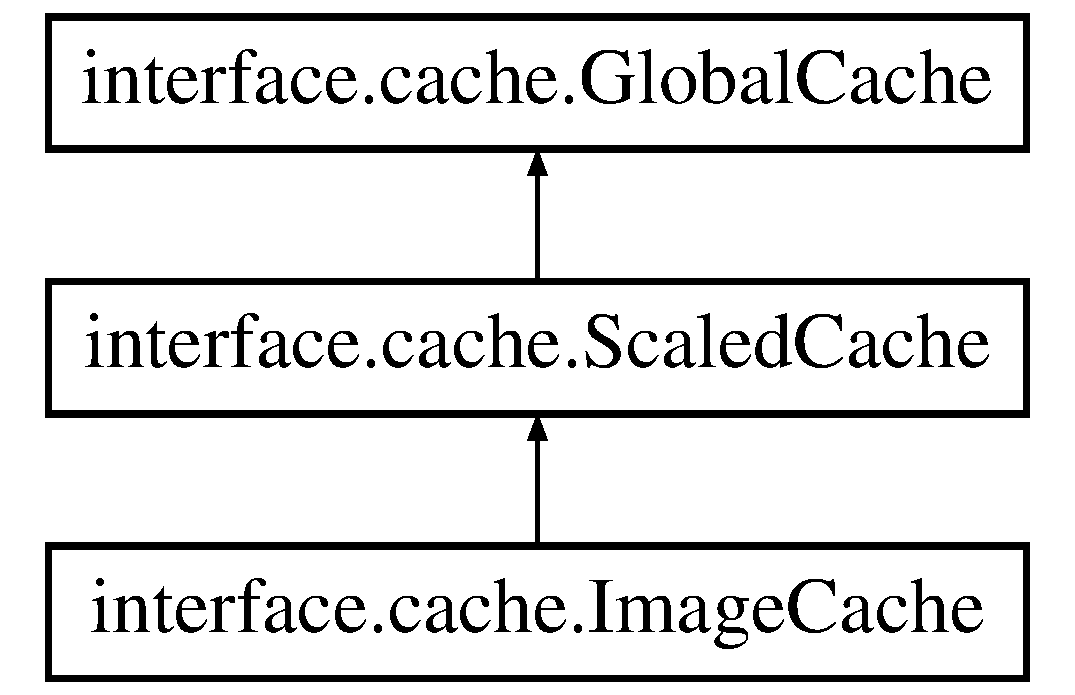
\includegraphics[height=3.000000cm]{classinterface_1_1cache_1_1_image_cache}
\end{center}
\end{figure}
\subsection*{\-Public \-Member \-Functions}
\begin{DoxyCompactItemize}
\item 
\hypertarget{classinterface_1_1cache_1_1_image_cache_a67306e2a9935733fa2b3f1fd30e74bf4}{def {\bfseries init\-\_\-image\-\_\-from\-\_\-file}}\label{classinterface_1_1cache_1_1_image_cache_a67306e2a9935733fa2b3f1fd30e74bf4}

\item 
\hypertarget{classinterface_1_1cache_1_1_image_cache_ae7ded9ebcbc43075f3c4d67f3f39b020}{def {\bfseries init\-\_\-image\-\_\-from\-\_\-surface}}\label{classinterface_1_1cache_1_1_image_cache_ae7ded9ebcbc43075f3c4d67f3f39b020}

\item 
\hypertarget{classinterface_1_1cache_1_1_image_cache_a585d1a6c7e619565d902e2d80627e24e}{def {\bfseries get\-\_\-image}}\label{classinterface_1_1cache_1_1_image_cache_a585d1a6c7e619565d902e2d80627e24e}

\item 
\hypertarget{classinterface_1_1cache_1_1_image_cache_aeb0d1c68b68729835c8e676e5837808f}{def {\bfseries init\-\_\-elts}}\label{classinterface_1_1cache_1_1_image_cache_aeb0d1c68b68729835c8e676e5837808f}

\item 
\hypertarget{classinterface_1_1cache_1_1_image_cache_a139077e504325b568f90930de7c3aca8}{def {\bfseries init\-\_\-images}}\label{classinterface_1_1cache_1_1_image_cache_a139077e504325b568f90930de7c3aca8}

\item 
\hypertarget{classinterface_1_1cache_1_1_image_cache_a8256c527238b39f23b8f606439114122}{def {\bfseries add\-\_\-scaled}}\label{classinterface_1_1cache_1_1_image_cache_a8256c527238b39f23b8f606439114122}

\end{DoxyCompactItemize}
\subsection*{\-Static \-Public \-Attributes}
\begin{DoxyCompactItemize}
\item 
\hypertarget{classinterface_1_1cache_1_1_image_cache_afa394e30aa08b02c7ead02a0f9dd448c}{dictionary {\bfseries cache} = \{\}}\label{classinterface_1_1cache_1_1_image_cache_afa394e30aa08b02c7ead02a0f9dd448c}

\end{DoxyCompactItemize}


\subsection{\-Detailed \-Description}
\begin{DoxyVerb}
Cache containing loaded images at different scales for direct use
in the game.
\end{DoxyVerb}
 

\-The documentation for this class was generated from the following file\-:\begin{DoxyCompactItemize}
\item 
src/interface/cache.\-py\end{DoxyCompactItemize}

\hypertarget{classinterface_1_1interactions_1_1_interaction}{\section{interface.\-interactions.\-Interaction \-Class \-Reference}
\label{classinterface_1_1interactions_1_1_interaction}\index{interface.\-interactions.\-Interaction@{interface.\-interactions.\-Interaction}}
}
\subsection*{\-Public \-Member \-Functions}
\begin{DoxyCompactItemize}
\item 
\hypertarget{classinterface_1_1interactions_1_1_interaction_a8e24342fbab9b8508ab2c037cb2facf0}{def {\bfseries \-\_\-\-\_\-init\-\_\-\-\_\-}}\label{classinterface_1_1interactions_1_1_interaction_a8e24342fbab9b8508ab2c037cb2facf0}

\item 
\hypertarget{classinterface_1_1interactions_1_1_interaction_a077e8944f45e377ad3e6c225a545aa86}{def {\bfseries load}}\label{classinterface_1_1interactions_1_1_interaction_a077e8944f45e377ad3e6c225a545aa86}

\end{DoxyCompactItemize}
\subsection*{\-Public \-Attributes}
\begin{DoxyCompactItemize}
\item 
\hypertarget{classinterface_1_1interactions_1_1_interaction_a00cd1dee9a8dba184edb37428380bb92}{{\bfseries target}}\label{classinterface_1_1interactions_1_1_interaction_a00cd1dee9a8dba184edb37428380bb92}

\item 
\hypertarget{classinterface_1_1interactions_1_1_interaction_afae7611b19a4850489268d42de12281d}{{\bfseries type}}\label{classinterface_1_1interactions_1_1_interaction_afae7611b19a4850489268d42de12281d}

\item 
\hypertarget{classinterface_1_1interactions_1_1_interaction_a684bc327719b7885001513805775aae7}{{\bfseries key}}\label{classinterface_1_1interactions_1_1_interaction_a684bc327719b7885001513805775aae7}

\item 
\hypertarget{classinterface_1_1interactions_1_1_interaction_aa0201055cceaccb25b7808f2e8f39856}{{\bfseries event}}\label{classinterface_1_1interactions_1_1_interaction_aa0201055cceaccb25b7808f2e8f39856}

\end{DoxyCompactItemize}


\subsection{\-Detailed \-Description}
\begin{DoxyVerb}Link between an user input and a event to trigger on a target \end{DoxyVerb}
 

\-The documentation for this class was generated from the following file\-:\begin{DoxyCompactItemize}
\item 
src/interface/interactions.\-py\end{DoxyCompactItemize}

\hypertarget{classinterface_1_1print_world_1_1_interface}{\section{interface.\-print\-World.\-Interface \-Class \-Reference}
\label{classinterface_1_1print_world_1_1_interface}\index{interface.\-print\-World.\-Interface@{interface.\-print\-World.\-Interface}}
}
\-Inheritance diagram for interface.\-print\-World.\-Interface\-:\begin{figure}[H]
\begin{center}
\leavevmode
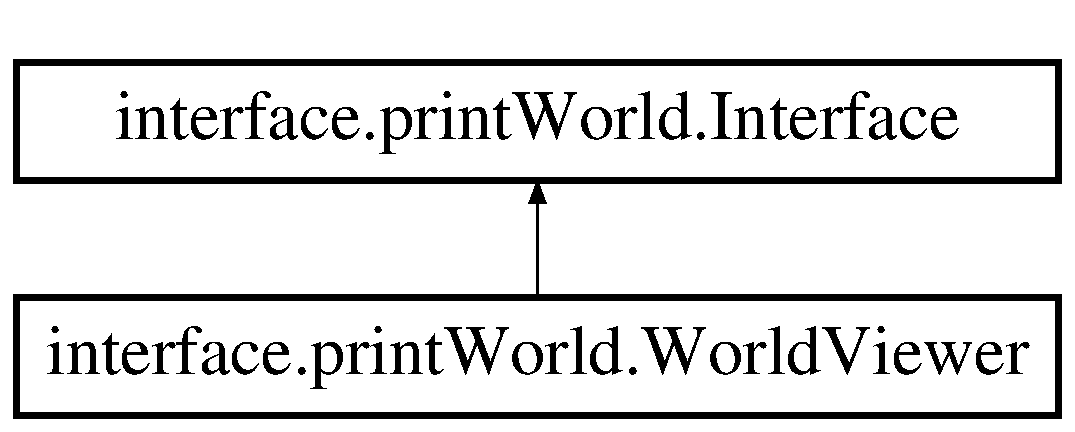
\includegraphics[height=2.000000cm]{classinterface_1_1print_world_1_1_interface}
\end{center}
\end{figure}


\-The documentation for this class was generated from the following file\-:\begin{DoxyCompactItemize}
\item 
src/interface/print\-World.\-py\end{DoxyCompactItemize}

\hypertarget{classinterface_1_1interface_1_1_interface}{\section{interface.\-interface.\-Interface \-Class \-Reference}
\label{classinterface_1_1interface_1_1_interface}\index{interface.\-interface.\-Interface@{interface.\-interface.\-Interface}}
}
\-Inheritance diagram for interface.\-interface.\-Interface\-:\begin{figure}[H]
\begin{center}
\leavevmode
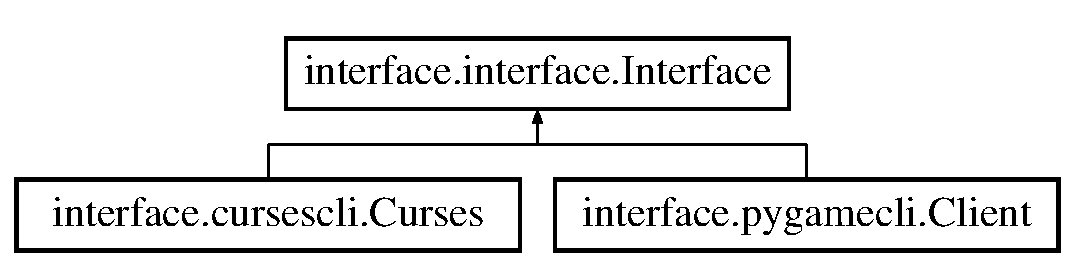
\includegraphics[height=2.000000cm]{classinterface_1_1interface_1_1_interface}
\end{center}
\end{figure}
\subsection*{\-Public \-Member \-Functions}
\begin{DoxyCompactItemize}
\item 
\hypertarget{classinterface_1_1interface_1_1_interface_ac897e94279885c6ac7368b26280b1ca3}{def {\bfseries \-\_\-\-\_\-init\-\_\-\-\_\-}}\label{classinterface_1_1interface_1_1_interface_ac897e94279885c6ac7368b26280b1ca3}

\item 
def \hyperlink{classinterface_1_1interface_1_1_interface_ae88eadf76465fc08de5b43ceb851b33c}{update}
\item 
\hypertarget{classinterface_1_1interface_1_1_interface_af98554929f55ff181f077938c49be445}{def {\bfseries repaint}}\label{classinterface_1_1interface_1_1_interface_af98554929f55ff181f077938c49be445}

\item 
\hypertarget{classinterface_1_1interface_1_1_interface_a5d5d771f07df8593a3c9a16b3c93cf87}{def {\bfseries set\-Perso}}\label{classinterface_1_1interface_1_1_interface_a5d5d771f07df8593a3c9a16b3c93cf87}

\item 
\hypertarget{classinterface_1_1interface_1_1_interface_a65d6c992d5c9ffe07bec1b57b05f171c}{def {\bfseries init}}\label{classinterface_1_1interface_1_1_interface_a65d6c992d5c9ffe07bec1b57b05f171c}

\item 
\hypertarget{classinterface_1_1interface_1_1_interface_aad5e69ce9ff8080f12d744ca1d7e31d9}{def {\bfseries end}}\label{classinterface_1_1interface_1_1_interface_aad5e69ce9ff8080f12d744ca1d7e31d9}

\item 
\hypertarget{classinterface_1_1interface_1_1_interface_af1f6baa08b21da6eb3458f91b9fc43a6}{def {\bfseries get\-Event}}\label{classinterface_1_1interface_1_1_interface_af1f6baa08b21da6eb3458f91b9fc43a6}

\end{DoxyCompactItemize}
\subsection*{\-Public \-Attributes}
\begin{DoxyCompactItemize}
\item 
\hypertarget{classinterface_1_1interface_1_1_interface_aa48bb41df8a8ef635c6d5fd9a3f1b502}{{\bfseries world}}\label{classinterface_1_1interface_1_1_interface_aa48bb41df8a8ef635c6d5fd9a3f1b502}

\item 
\hypertarget{classinterface_1_1interface_1_1_interface_ae09dfa2d4e610bbcf7315357f4b6ff7c}{{\bfseries last\-Update}}\label{classinterface_1_1interface_1_1_interface_ae09dfa2d4e610bbcf7315357f4b6ff7c}

\item 
\hypertarget{classinterface_1_1interface_1_1_interface_ad64363a847c04ef733dcf432f7900b80}{{\bfseries plugins}}\label{classinterface_1_1interface_1_1_interface_ad64363a847c04ef733dcf432f7900b80}

\item 
\hypertarget{classinterface_1_1interface_1_1_interface_a34c17b9a544613b17c4c4739650cb406}{{\bfseries images}}\label{classinterface_1_1interface_1_1_interface_a34c17b9a544613b17c4c4739650cb406}

\end{DoxyCompactItemize}


\subsection{\-Detailed \-Description}
\begin{DoxyVerb}UI base-class, can be used as a dummy interface \end{DoxyVerb}
 

\subsection{\-Member \-Function \-Documentation}
\hypertarget{classinterface_1_1interface_1_1_interface_ae88eadf76465fc08de5b43ceb851b33c}{\index{interface\-::interface\-::\-Interface@{interface\-::interface\-::\-Interface}!update@{update}}
\index{update@{update}!interface::interface::Interface@{interface\-::interface\-::\-Interface}}
\subsubsection[{update}]{\setlength{\rightskip}{0pt plus 5cm}def {\bf interface.\-interface.\-Interface.\-update} (
\begin{DoxyParamCaption}
\item[{}]{self}
\end{DoxyParamCaption}
)}}\label{classinterface_1_1interface_1_1_interface_ae88eadf76465fc08de5b43ceb851b33c}
\begin{DoxyVerb}Update the UI \end{DoxyVerb}
 

\-The documentation for this class was generated from the following file\-:\begin{DoxyCompactItemize}
\item 
src/interface/interface.\-py\end{DoxyCompactItemize}

\hypertarget{classinterface_1_1layer_1_1_layer}{\section{interface.\-layer.\-Layer \-Class \-Reference}
\label{classinterface_1_1layer_1_1_layer}\index{interface.\-layer.\-Layer@{interface.\-layer.\-Layer}}
}
\-Inheritance diagram for interface.\-layer.\-Layer\-:\begin{figure}[H]
\begin{center}
\leavevmode
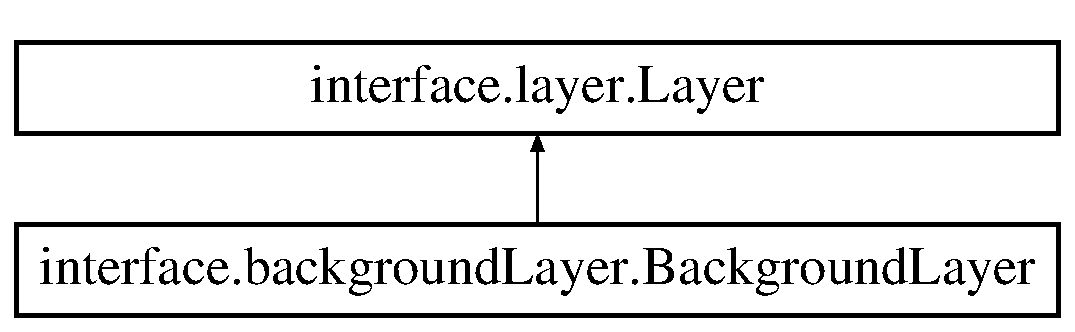
\includegraphics[height=2.000000cm]{classinterface_1_1layer_1_1_layer}
\end{center}
\end{figure}
\subsection*{\-Public \-Member \-Functions}
\begin{DoxyCompactItemize}
\item 
\hypertarget{classinterface_1_1layer_1_1_layer_ab9b02ee5672b0222065ac7d8148b6c9c}{def {\bfseries \-\_\-\-\_\-init\-\_\-\-\_\-}}\label{classinterface_1_1layer_1_1_layer_ab9b02ee5672b0222065ac7d8148b6c9c}

\item 
\hypertarget{classinterface_1_1layer_1_1_layer_ae5bf1cf30133971912c978524741098e}{def {\bfseries render}}\label{classinterface_1_1layer_1_1_layer_ae5bf1cf30133971912c978524741098e}

\item 
\hypertarget{classinterface_1_1layer_1_1_layer_a6e98a961961ea7d430adac46d3c29719}{def {\bfseries update}}\label{classinterface_1_1layer_1_1_layer_a6e98a961961ea7d430adac46d3c29719}

\item 
\hypertarget{classinterface_1_1layer_1_1_layer_a5b1411d03b84e5b0d0a86a6c58eba3a5}{def {\bfseries get\-\_\-cell\-\_\-pos}}\label{classinterface_1_1layer_1_1_layer_a5b1411d03b84e5b0d0a86a6c58eba3a5}

\item 
def \hyperlink{classinterface_1_1layer_1_1_layer_a36c73749e127ff1d97ca205cd544c07d}{make\-\_\-grid}
\end{DoxyCompactItemize}
\subsection*{\-Public \-Attributes}
\begin{DoxyCompactItemize}
\item 
\hypertarget{classinterface_1_1layer_1_1_layer_ae1bebea05562b4b4a370055b1b46d6f7}{{\bfseries cells}}\label{classinterface_1_1layer_1_1_layer_ae1bebea05562b4b4a370055b1b46d6f7}

\item 
\hypertarget{classinterface_1_1layer_1_1_layer_a4031353d183640938e4f5c6ff24f70b9}{{\bfseries g\-\_\-width}}\label{classinterface_1_1layer_1_1_layer_a4031353d183640938e4f5c6ff24f70b9}

\item 
\hypertarget{classinterface_1_1layer_1_1_layer_a7b6de244f592dc3194a71ee696ff7d25}{{\bfseries g\-\_\-height}}\label{classinterface_1_1layer_1_1_layer_a7b6de244f592dc3194a71ee696ff7d25}

\item 
\hypertarget{classinterface_1_1layer_1_1_layer_a23dcea50c96c37299dedd45fb40e5253}{{\bfseries size}}\label{classinterface_1_1layer_1_1_layer_a23dcea50c96c37299dedd45fb40e5253}

\end{DoxyCompactItemize}


\subsection{\-Detailed \-Description}
\begin{DoxyVerb}A abstract class defining a layer of the display (ex. background) \end{DoxyVerb}
 

\subsection{\-Member \-Function \-Documentation}
\hypertarget{classinterface_1_1layer_1_1_layer_a36c73749e127ff1d97ca205cd544c07d}{\index{interface\-::layer\-::\-Layer@{interface\-::layer\-::\-Layer}!make\-\_\-grid@{make\-\_\-grid}}
\index{make\-\_\-grid@{make\-\_\-grid}!interface::layer::Layer@{interface\-::layer\-::\-Layer}}
\subsubsection[{make\-\_\-grid}]{\setlength{\rightskip}{0pt plus 5cm}def {\bf interface.\-layer.\-Layer.\-make\-\_\-grid} (
\begin{DoxyParamCaption}
\item[{}]{self, }
\item[{}]{img\-\_\-set, }
\item[{}]{cell\-\_\-ids}
\end{DoxyParamCaption}
)}}\label{classinterface_1_1layer_1_1_layer_a36c73749e127ff1d97ca205cd544c07d}
\begin{DoxyVerb}
Build the grid that will be drawn by Pygame. Img_set is a list
of (id/type, filename) specifying the files to load for each type
of cell and cell_ids is the type for each cell.
\end{DoxyVerb}
 

\-The documentation for this class was generated from the following file\-:\begin{DoxyCompactItemize}
\item 
src/interface/layer.\-py\end{DoxyCompactItemize}

\hypertarget{classworld_1_1_map}{\section{world.\-Map \-Class \-Reference}
\label{classworld_1_1_map}\index{world.\-Map@{world.\-Map}}
}
\-Inheritance diagram for world.\-Map\-:\begin{figure}[H]
\begin{center}
\leavevmode
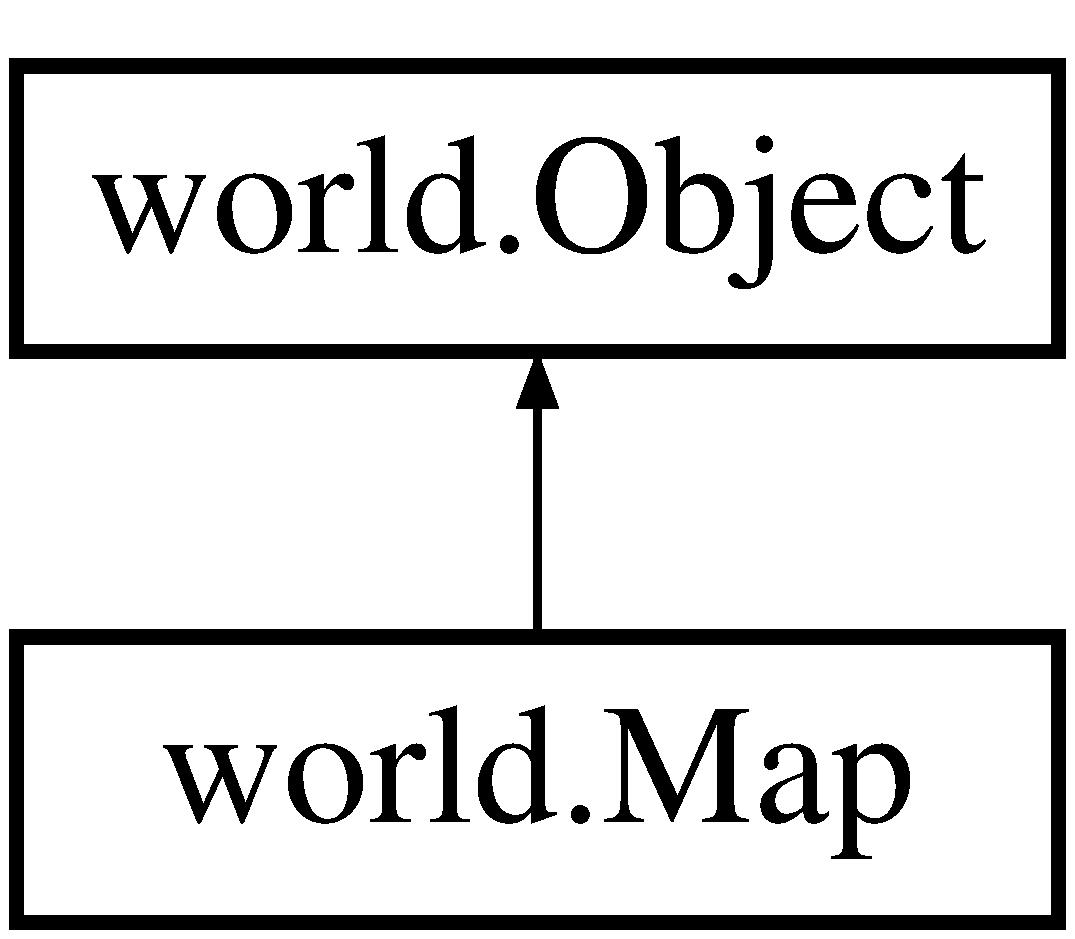
\includegraphics[height=2.000000cm]{classworld_1_1_map}
\end{center}
\end{figure}
\subsection*{\-Public \-Member \-Functions}
\begin{DoxyCompactItemize}
\item 
\hypertarget{classworld_1_1_map_aabfde95675f6b82d9a8afcd676053632}{def {\bfseries \-\_\-\-\_\-init\-\_\-\-\_\-}}\label{classworld_1_1_map_aabfde95675f6b82d9a8afcd676053632}

\item 
def \hyperlink{classworld_1_1_map_ac8e650b696f537d9df20ee5d2243e978}{fill}
\item 
def \hyperlink{classworld_1_1_map_ac5f255ae58db6b391d0a3d5807365370}{dist}
\item 
def \hyperlink{classworld_1_1_map_a7b1d3e4419fd5bd48d5f759e63ae55f5}{lov}
\item 
def \hyperlink{classworld_1_1_map_aabdd46688167e96753c73df0f0486588}{get\-\_\-path}
\item 
def \hyperlink{classworld_1_1_map_a12e89884cc3e9da4d024575a85b1d324}{from\-Pos}
\end{DoxyCompactItemize}
\subsection*{\-Public \-Attributes}
\begin{DoxyCompactItemize}
\item 
\hypertarget{classworld_1_1_map_af412cfb2a5b25f4ca3188498f916a647}{{\bfseries cells}}\label{classworld_1_1_map_af412cfb2a5b25f4ca3188498f916a647}

\item 
\hypertarget{classworld_1_1_map_aec6e18657e8d65b1ab57cdf305e2de37}{{\bfseries cells\-Grid}}\label{classworld_1_1_map_aec6e18657e8d65b1ab57cdf305e2de37}

\end{DoxyCompactItemize}


\subsection{\-Detailed \-Description}
\begin{DoxyVerb}Orthonormed map with associated alogrithms \end{DoxyVerb}
 

\subsection{\-Member \-Function \-Documentation}
\hypertarget{classworld_1_1_map_ac5f255ae58db6b391d0a3d5807365370}{\index{world\-::\-Map@{world\-::\-Map}!dist@{dist}}
\index{dist@{dist}!world::Map@{world\-::\-Map}}
\subsubsection[{dist}]{\setlength{\rightskip}{0pt plus 5cm}def {\bf world.\-Map.\-dist} (
\begin{DoxyParamCaption}
\item[{}]{self, }
\item[{}]{source, }
\item[{}]{dest}
\end{DoxyParamCaption}
)}}\label{classworld_1_1_map_ac5f255ae58db6b391d0a3d5807365370}
\begin{DoxyVerb}Manhattan distance \end{DoxyVerb}
 \hypertarget{classworld_1_1_map_ac8e650b696f537d9df20ee5d2243e978}{\index{world\-::\-Map@{world\-::\-Map}!fill@{fill}}
\index{fill@{fill}!world::Map@{world\-::\-Map}}
\subsubsection[{fill}]{\setlength{\rightskip}{0pt plus 5cm}def {\bf world.\-Map.\-fill} (
\begin{DoxyParamCaption}
\item[{}]{self}
\end{DoxyParamCaption}
)}}\label{classworld_1_1_map_ac8e650b696f537d9df20ee5d2243e978}
\begin{DoxyVerb}Fill the cellsGrid attribute with cells and default cell
To be called after the Xml reading only \end{DoxyVerb}
 \hypertarget{classworld_1_1_map_a12e89884cc3e9da4d024575a85b1d324}{\index{world\-::\-Map@{world\-::\-Map}!from\-Pos@{from\-Pos}}
\index{from\-Pos@{from\-Pos}!world::Map@{world\-::\-Map}}
\subsubsection[{from\-Pos}]{\setlength{\rightskip}{0pt plus 5cm}def {\bf world.\-Map.\-from\-Pos} (
\begin{DoxyParamCaption}
\item[{}]{self, }
\item[{}]{pos, }
\item[{}]{maxi = {\ttfamily \-None}}
\end{DoxyParamCaption}
)}}\label{classworld_1_1_map_a12e89884cc3e9da4d024575a85b1d324}
\begin{DoxyVerb}Yield cells further and further from pos, stopping at maxi
Assuming x goes right and y down it turns as the trigo circle,
it is therefore not a "serpentin" (sadly ?) \end{DoxyVerb}
 \hypertarget{classworld_1_1_map_aabdd46688167e96753c73df0f0486588}{\index{world\-::\-Map@{world\-::\-Map}!get\-\_\-path@{get\-\_\-path}}
\index{get\-\_\-path@{get\-\_\-path}!world::Map@{world\-::\-Map}}
\subsubsection[{get\-\_\-path}]{\setlength{\rightskip}{0pt plus 5cm}def {\bf world.\-Map.\-get\-\_\-path} (
\begin{DoxyParamCaption}
\item[{}]{self, }
\item[{}]{source, }
\item[{}]{dest}
\end{DoxyParamCaption}
)}}\label{classworld_1_1_map_aabdd46688167e96753c73df0f0486588}
\begin{DoxyVerb}A* algorithm on current map from source to dest \end{DoxyVerb}
 \hypertarget{classworld_1_1_map_a7b1d3e4419fd5bd48d5f759e63ae55f5}{\index{world\-::\-Map@{world\-::\-Map}!lov@{lov}}
\index{lov@{lov}!world::Map@{world\-::\-Map}}
\subsubsection[{lov}]{\setlength{\rightskip}{0pt plus 5cm}def {\bf world.\-Map.\-lov} (
\begin{DoxyParamCaption}
\item[{}]{self, }
\item[{}]{source, }
\item[{}]{dest}
\end{DoxyParamCaption}
)}}\label{classworld_1_1_map_a7b1d3e4419fd5bd48d5f759e63ae55f5}
\begin{DoxyVerb}Computes if the view is degaged between source and dest
those laters must have x and y parameters and the map
cells a parameter "visible"
About O(dist(source, dest))
\end{DoxyVerb}
 

\-The documentation for this class was generated from the following file\-:\begin{DoxyCompactItemize}
\item 
src/shared/world.\-py\end{DoxyCompactItemize}

\hypertarget{classinterface_1_1cursescli_1_1_map_view}{\section{interface.\-cursescli.\-Map\-View \-Class \-Reference}
\label{classinterface_1_1cursescli_1_1_map_view}\index{interface.\-cursescli.\-Map\-View@{interface.\-cursescli.\-Map\-View}}
}
\subsection*{\-Public \-Member \-Functions}
\begin{DoxyCompactItemize}
\item 
\hypertarget{classinterface_1_1cursescli_1_1_map_view_ab01484a5b5c8ca9d5c779bee1ef6d710}{def {\bfseries \-\_\-\-\_\-init\-\_\-\-\_\-}}\label{classinterface_1_1cursescli_1_1_map_view_ab01484a5b5c8ca9d5c779bee1ef6d710}

\item 
\hypertarget{classinterface_1_1cursescli_1_1_map_view_ae4868812e622acf9cb0da05ecbd17ea5}{def {\bfseries set\-Win}}\label{classinterface_1_1cursescli_1_1_map_view_ae4868812e622acf9cb0da05ecbd17ea5}

\item 
def \hyperlink{classinterface_1_1cursescli_1_1_map_view_ad761d937ddcdad5ed32cdcbccc70cbb1}{update\-Map}
\item 
\hypertarget{classinterface_1_1cursescli_1_1_map_view_a73a675f44f28cfae9a11f631fa7a972b}{def {\bfseries draw}}\label{classinterface_1_1cursescli_1_1_map_view_a73a675f44f28cfae9a11f631fa7a972b}

\item 
def \hyperlink{classinterface_1_1cursescli_1_1_map_view_acf3f62c908193e8f80710f78af3ef8a6}{cell\-Char}
\item 
def \hyperlink{classinterface_1_1cursescli_1_1_map_view_a7365f14995f5e7edb9fe110e65080672}{clip\-Offset}
\item 
\hypertarget{classinterface_1_1cursescli_1_1_map_view_a37487d0d1d8a28471673c3f7b456f1dc}{def {\bfseries handle\-Key}}\label{classinterface_1_1cursescli_1_1_map_view_a37487d0d1d8a28471673c3f7b456f1dc}

\item 
def \hyperlink{classinterface_1_1cursescli_1_1_map_view_aa1bdbf7ace6bbaebec6896e8742d3641}{fast\-Lov}
\end{DoxyCompactItemize}
\subsection*{\-Public \-Attributes}
\begin{DoxyCompactItemize}
\item 
\hypertarget{classinterface_1_1cursescli_1_1_map_view_a7bff77612dcfe3035387e99db71f3690}{{\bfseries world}}\label{classinterface_1_1cursescli_1_1_map_view_a7bff77612dcfe3035387e99db71f3690}

\item 
\hypertarget{classinterface_1_1cursescli_1_1_map_view_ad93c97660df9a460d2ff8ec8222be817}{{\bfseries off\-X}}\label{classinterface_1_1cursescli_1_1_map_view_ad93c97660df9a460d2ff8ec8222be817}

\item 
\hypertarget{classinterface_1_1cursescli_1_1_map_view_aa2be0a9143e3e9ae7a50497f969f1415}{{\bfseries off\-Y}}\label{classinterface_1_1cursescli_1_1_map_view_aa2be0a9143e3e9ae7a50497f969f1415}

\item 
\hypertarget{classinterface_1_1cursescli_1_1_map_view_a699cbd4485523dd2faabcedf9668f5c7}{{\bfseries map}}\label{classinterface_1_1cursescli_1_1_map_view_a699cbd4485523dd2faabcedf9668f5c7}

\item 
\hypertarget{classinterface_1_1cursescli_1_1_map_view_a0994b492a53b0a0b95012dd4fd07faaf}{{\bfseries show\-Lov}}\label{classinterface_1_1cursescli_1_1_map_view_a0994b492a53b0a0b95012dd4fd07faaf}

\item 
\hypertarget{classinterface_1_1cursescli_1_1_map_view_a27b2404378d54503cc18b80d55f8be97}{{\bfseries perso}}\label{classinterface_1_1cursescli_1_1_map_view_a27b2404378d54503cc18b80d55f8be97}

\item 
\hypertarget{classinterface_1_1cursescli_1_1_map_view_ab3bc4fc81b249a6a978638afed446352}{{\bfseries follow}}\label{classinterface_1_1cursescli_1_1_map_view_ab3bc4fc81b249a6a978638afed446352}

\item 
\hypertarget{classinterface_1_1cursescli_1_1_map_view_abf0f9588c017457121c18d929f8cf175}{{\bfseries win}}\label{classinterface_1_1cursescli_1_1_map_view_abf0f9588c017457121c18d929f8cf175}

\item 
\hypertarget{classinterface_1_1cursescli_1_1_map_view_af2ad8dfaad4433e0e4e9e8d906ca1e4a}{{\bfseries max\-Width}}\label{classinterface_1_1cursescli_1_1_map_view_af2ad8dfaad4433e0e4e9e8d906ca1e4a}

\item 
\hypertarget{classinterface_1_1cursescli_1_1_map_view_a89ce02532a85956e4ed40d542a8dee05}{{\bfseries height}}\label{classinterface_1_1cursescli_1_1_map_view_a89ce02532a85956e4ed40d542a8dee05}

\item 
\hypertarget{classinterface_1_1cursescli_1_1_map_view_a43149a1b807de32ab262bd356955b842}{{\bfseries width}}\label{classinterface_1_1cursescli_1_1_map_view_a43149a1b807de32ab262bd356955b842}

\item 
\hypertarget{classinterface_1_1cursescli_1_1_map_view_ae22ec0cc3de12de2abc3df53b4838b27}{{\bfseries lovs}}\label{classinterface_1_1cursescli_1_1_map_view_ae22ec0cc3de12de2abc3df53b4838b27}

\end{DoxyCompactItemize}


\subsection{\-Detailed \-Description}
\begin{DoxyVerb}Manages the map display \end{DoxyVerb}
 

\subsection{\-Member \-Function \-Documentation}
\hypertarget{classinterface_1_1cursescli_1_1_map_view_acf3f62c908193e8f80710f78af3ef8a6}{\index{interface\-::cursescli\-::\-Map\-View@{interface\-::cursescli\-::\-Map\-View}!cell\-Char@{cell\-Char}}
\index{cell\-Char@{cell\-Char}!interface::cursescli::MapView@{interface\-::cursescli\-::\-Map\-View}}
\subsubsection[{cell\-Char}]{\setlength{\rightskip}{0pt plus 5cm}def {\bf interface.\-cursescli.\-Map\-View.\-cell\-Char} (
\begin{DoxyParamCaption}
\item[{}]{self, }
\item[{}]{cell}
\end{DoxyParamCaption}
)}}\label{classinterface_1_1cursescli_1_1_map_view_acf3f62c908193e8f80710f78af3ef8a6}
\begin{DoxyVerb}Return the char associated to a cell and some overlays \end{DoxyVerb}
 \hypertarget{classinterface_1_1cursescli_1_1_map_view_a7365f14995f5e7edb9fe110e65080672}{\index{interface\-::cursescli\-::\-Map\-View@{interface\-::cursescli\-::\-Map\-View}!clip\-Offset@{clip\-Offset}}
\index{clip\-Offset@{clip\-Offset}!interface::cursescli::MapView@{interface\-::cursescli\-::\-Map\-View}}
\subsubsection[{clip\-Offset}]{\setlength{\rightskip}{0pt plus 5cm}def {\bf interface.\-cursescli.\-Map\-View.\-clip\-Offset} (
\begin{DoxyParamCaption}
\item[{}]{self}
\end{DoxyParamCaption}
)}}\label{classinterface_1_1cursescli_1_1_map_view_a7365f14995f5e7edb9fe110e65080672}
\begin{DoxyVerb}Ensure the offX, offY lead to a valid display \end{DoxyVerb}
 \hypertarget{classinterface_1_1cursescli_1_1_map_view_aa1bdbf7ace6bbaebec6896e8742d3641}{\index{interface\-::cursescli\-::\-Map\-View@{interface\-::cursescli\-::\-Map\-View}!fast\-Lov@{fast\-Lov}}
\index{fast\-Lov@{fast\-Lov}!interface::cursescli::MapView@{interface\-::cursescli\-::\-Map\-View}}
\subsubsection[{fast\-Lov}]{\setlength{\rightskip}{0pt plus 5cm}def {\bf interface.\-cursescli.\-Map\-View.\-fast\-Lov} (
\begin{DoxyParamCaption}
\item[{}]{self}
\end{DoxyParamCaption}
)}}\label{classinterface_1_1cursescli_1_1_map_view_aa1bdbf7ace6bbaebec6896e8742d3641}
\begin{DoxyVerb}as Map.lov but optimised for a zone ~O(cellNumber)
rather fluid up to 20.000 cells \end{DoxyVerb}
 \hypertarget{classinterface_1_1cursescli_1_1_map_view_ad761d937ddcdad5ed32cdcbccc70cbb1}{\index{interface\-::cursescli\-::\-Map\-View@{interface\-::cursescli\-::\-Map\-View}!update\-Map@{update\-Map}}
\index{update\-Map@{update\-Map}!interface::cursescli::MapView@{interface\-::cursescli\-::\-Map\-View}}
\subsubsection[{update\-Map}]{\setlength{\rightskip}{0pt plus 5cm}def {\bf interface.\-cursescli.\-Map\-View.\-update\-Map} (
\begin{DoxyParamCaption}
\item[{}]{self}
\end{DoxyParamCaption}
)}}\label{classinterface_1_1cursescli_1_1_map_view_ad761d937ddcdad5ed32cdcbccc70cbb1}
\begin{DoxyVerb}Center map in the window \end{DoxyVerb}
 

\-The documentation for this class was generated from the following file\-:\begin{DoxyCompactItemize}
\item 
src/interface/cursescli.\-py\end{DoxyCompactItemize}

\hypertarget{classinterface_1_1map_1_1_map_viewer}{\section{interface.\-map.\-Map\-Viewer \-Class \-Reference}
\label{classinterface_1_1map_1_1_map_viewer}\index{interface.\-map.\-Map\-Viewer@{interface.\-map.\-Map\-Viewer}}
}
\subsection*{\-Public \-Member \-Functions}
\begin{DoxyCompactItemize}
\item 
\hypertarget{classinterface_1_1map_1_1_map_viewer_adbed7cbe4a6078d5bc3cd8232990e0b3}{def {\bfseries \-\_\-\-\_\-init\-\_\-\-\_\-}}\label{classinterface_1_1map_1_1_map_viewer_adbed7cbe4a6078d5bc3cd8232990e0b3}

\item 
\hypertarget{classinterface_1_1map_1_1_map_viewer_a950c4e78dd52d72f05578fbc907f55c3}{def {\bfseries load\-\_\-chunks}}\label{classinterface_1_1map_1_1_map_viewer_a950c4e78dd52d72f05578fbc907f55c3}

\item 
\hypertarget{classinterface_1_1map_1_1_map_viewer_ab1a87ccdc662aa25e277c145811f35e1}{def {\bfseries make\-\_\-walkables}}\label{classinterface_1_1map_1_1_map_viewer_ab1a87ccdc662aa25e277c145811f35e1}

\item 
\hypertarget{classinterface_1_1map_1_1_map_viewer_a6627b670006580b8a0bd0a3400100e2c}{def {\bfseries zoom}}\label{classinterface_1_1map_1_1_map_viewer_a6627b670006580b8a0bd0a3400100e2c}

\item 
\hypertarget{classinterface_1_1map_1_1_map_viewer_ae77159080d71d007d22a7ca876ebddb5}{def {\bfseries move}}\label{classinterface_1_1map_1_1_map_viewer_ae77159080d71d007d22a7ca876ebddb5}

\item 
\hypertarget{classinterface_1_1map_1_1_map_viewer_a79d3cd7b3210dfb15781d42f2954f08a}{def {\bfseries render}}\label{classinterface_1_1map_1_1_map_viewer_a79d3cd7b3210dfb15781d42f2954f08a}

\item 
\hypertarget{classinterface_1_1map_1_1_map_viewer_a003c479abb34df98d252344fa28e3f5b}{def {\bfseries onscreen\-\_\-chunks}}\label{classinterface_1_1map_1_1_map_viewer_a003c479abb34df98d252344fa28e3f5b}

\item 
\hypertarget{classinterface_1_1map_1_1_map_viewer_a8ecc5a5202e22765415400132ec76bf4}{def {\bfseries update}}\label{classinterface_1_1map_1_1_map_viewer_a8ecc5a5202e22765415400132ec76bf4}

\item 
\hypertarget{classinterface_1_1map_1_1_map_viewer_a7be5a084dbdae9da3b27121b2386d393}{def {\bfseries update\-\_\-chunks}}\label{classinterface_1_1map_1_1_map_viewer_a7be5a084dbdae9da3b27121b2386d393}

\item 
\hypertarget{classinterface_1_1map_1_1_map_viewer_a13c1ba55acebf6b532236214e3bc5334}{def {\bfseries propagate\-\_\-trigger}}\label{classinterface_1_1map_1_1_map_viewer_a13c1ba55acebf6b532236214e3bc5334}

\item 
\hypertarget{classinterface_1_1map_1_1_map_viewer_add4eeba2a77785384aa29070dba5c1c7}{def {\bfseries compute\-\_\-path}}\label{classinterface_1_1map_1_1_map_viewer_add4eeba2a77785384aa29070dba5c1c7}

\item 
\hypertarget{classinterface_1_1map_1_1_map_viewer_a28fd1b7e0f84b29a97aea2d434dec953}{def {\bfseries load\-\_\-bg}}\label{classinterface_1_1map_1_1_map_viewer_a28fd1b7e0f84b29a97aea2d434dec953}

\end{DoxyCompactItemize}
\subsection*{\-Public \-Attributes}
\begin{DoxyCompactItemize}
\item 
\hypertarget{classinterface_1_1map_1_1_map_viewer_a587ea56edafde8ffe575ced8dbec50e1}{{\bfseries map}}\label{classinterface_1_1map_1_1_map_viewer_a587ea56edafde8ffe575ced8dbec50e1}

\item 
\hypertarget{classinterface_1_1map_1_1_map_viewer_a61bc55a498d7cc634a22ee159288be8d}{{\bfseries world}}\label{classinterface_1_1map_1_1_map_viewer_a61bc55a498d7cc634a22ee159288be8d}

\item 
\hypertarget{classinterface_1_1map_1_1_map_viewer_acdb386d08c81742b4f23c7bd33e127e0}{{\bfseries cm\-\_\-height}}\label{classinterface_1_1map_1_1_map_viewer_acdb386d08c81742b4f23c7bd33e127e0}

\item 
\hypertarget{classinterface_1_1map_1_1_map_viewer_a1747b8a1f9c804ca2c67a19c710395fa}{{\bfseries width}}\label{classinterface_1_1map_1_1_map_viewer_a1747b8a1f9c804ca2c67a19c710395fa}

\item 
\hypertarget{classinterface_1_1map_1_1_map_viewer_aa7669efffc1b4a3bd4772c2727fd2380}{{\bfseries height}}\label{classinterface_1_1map_1_1_map_viewer_aa7669efffc1b4a3bd4772c2727fd2380}

\item 
\hypertarget{classinterface_1_1map_1_1_map_viewer_ab93d7790428ba1e83bcb7502e80e5dc8}{{\bfseries screen\-\_\-cgwidth}}\label{classinterface_1_1map_1_1_map_viewer_ab93d7790428ba1e83bcb7502e80e5dc8}

\item 
\hypertarget{classinterface_1_1map_1_1_map_viewer_af5b404f15cda737dc42926eb3862dee3}{{\bfseries screen\-\_\-cgheight}}\label{classinterface_1_1map_1_1_map_viewer_af5b404f15cda737dc42926eb3862dee3}

\item 
\hypertarget{classinterface_1_1map_1_1_map_viewer_aa4d567e0e0738b2138079c7d30b9b8a3}{{\bfseries walkables\-Graph}}\label{classinterface_1_1map_1_1_map_viewer_aa4d567e0e0738b2138079c7d30b9b8a3}

\item 
\hypertarget{classinterface_1_1map_1_1_map_viewer_aaacf1a066182f54e1a0fea0ed7e26f1a}{{\bfseries last\-\_\-curr\-\_\-chunk}}\label{classinterface_1_1map_1_1_map_viewer_aaacf1a066182f54e1a0fea0ed7e26f1a}

\item 
\hypertarget{classinterface_1_1map_1_1_map_viewer_a309b8238a920b2c71ce390ac45c3542a}{{\bfseries current\-\_\-chunk}}\label{classinterface_1_1map_1_1_map_viewer_a309b8238a920b2c71ce390ac45c3542a}

\item 
\hypertarget{classinterface_1_1map_1_1_map_viewer_a711222341d6a732bcfb524178856dce2}{{\bfseries pos\-\_\-offset}}\label{classinterface_1_1map_1_1_map_viewer_a711222341d6a732bcfb524178856dce2}

\item 
\hypertarget{classinterface_1_1map_1_1_map_viewer_a11b73fbd23f3a67c1aa1e58efafd3adf}{{\bfseries chunk\-\_\-pos}}\label{classinterface_1_1map_1_1_map_viewer_a11b73fbd23f3a67c1aa1e58efafd3adf}

\item 
\hypertarget{classinterface_1_1map_1_1_map_viewer_af959880445d83740669c6a44c52d0f8e}{{\bfseries chunks\-\_\-state}}\label{classinterface_1_1map_1_1_map_viewer_af959880445d83740669c6a44c52d0f8e}

\end{DoxyCompactItemize}


\-The documentation for this class was generated from the following file\-:\begin{DoxyCompactItemize}
\item 
src/interface/map.\-py\end{DoxyCompactItemize}

\hypertarget{classplugins_1_1menu_1_1_menu_view}{\section{plugins.\-menu.\-Menu\-View \-Class \-Reference}
\label{classplugins_1_1menu_1_1_menu_view}\index{plugins.\-menu.\-Menu\-View@{plugins.\-menu.\-Menu\-View}}
}
\-Inheritance diagram for plugins.\-menu.\-Menu\-View\-:\begin{figure}[H]
\begin{center}
\leavevmode
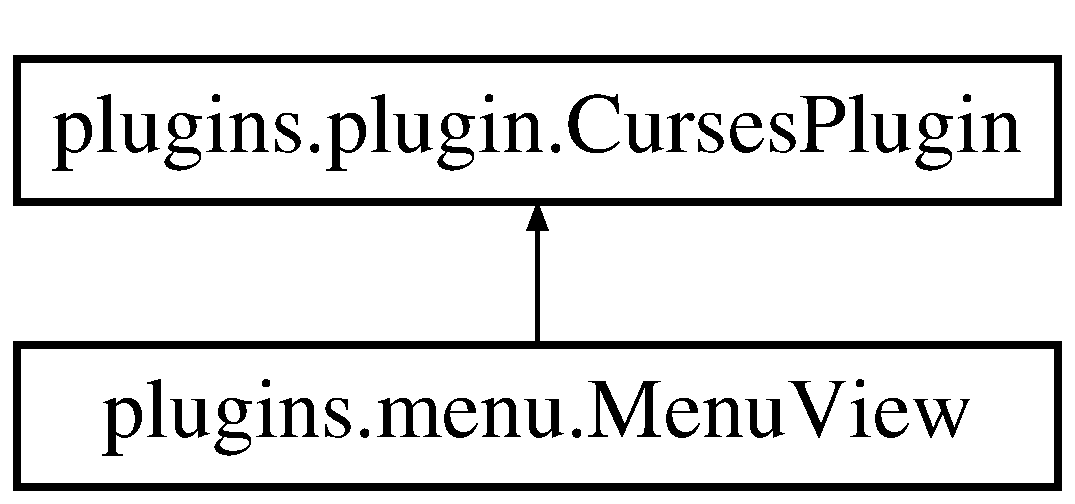
\includegraphics[height=2.000000cm]{classplugins_1_1menu_1_1_menu_view}
\end{center}
\end{figure}
\subsection*{\-Public \-Member \-Functions}
\begin{DoxyCompactItemize}
\item 
def \hyperlink{classplugins_1_1menu_1_1_menu_view_a693bc4021b2a04bd22ceb15dde01a330}{draw}
\item 
def \hyperlink{classplugins_1_1menu_1_1_menu_view_a259e6ac87d88f5d1ce17770ac46f5865}{centered}
\end{DoxyCompactItemize}
\subsection*{\-Static \-Public \-Attributes}
\begin{DoxyCompactItemize}
\item 
\hypertarget{classplugins_1_1menu_1_1_menu_view_ab3438cfcc2b703482d6d1ecab9679d66}{int {\bfseries \-M\-I\-N\-W} = 26}\label{classplugins_1_1menu_1_1_menu_view_ab3438cfcc2b703482d6d1ecab9679d66}

\item 
\hypertarget{classplugins_1_1menu_1_1_menu_view_a307f27961873f3d00395c2cd019a66cf}{int {\bfseries \-M\-I\-N\-H} = 1000}\label{classplugins_1_1menu_1_1_menu_view_a307f27961873f3d00395c2cd019a66cf}

\item 
\hypertarget{classplugins_1_1menu_1_1_menu_view_ab9c4a00d5b07171198ac2f6255dbca4a}{{\bfseries \-X} = -\/\-M\-I\-N\-W}\label{classplugins_1_1menu_1_1_menu_view_ab9c4a00d5b07171198ac2f6255dbca4a}

\item 
\hypertarget{classplugins_1_1menu_1_1_menu_view_aa138149f8ea669dacc4bed733952c76f}{int {\bfseries \-Y} = 0}\label{classplugins_1_1menu_1_1_menu_view_aa138149f8ea669dacc4bed733952c76f}

\item 
\hypertarget{classplugins_1_1menu_1_1_menu_view_a78be57e5f75c472e43e9907735035710}{string {\bfseries \-N\-A\-M\-E} = \char`\"{}\-Menu\char`\"{}}\label{classplugins_1_1menu_1_1_menu_view_a78be57e5f75c472e43e9907735035710}

\end{DoxyCompactItemize}


\subsection{\-Member \-Function \-Documentation}
\hypertarget{classplugins_1_1menu_1_1_menu_view_a259e6ac87d88f5d1ce17770ac46f5865}{\index{plugins\-::menu\-::\-Menu\-View@{plugins\-::menu\-::\-Menu\-View}!centered@{centered}}
\index{centered@{centered}!plugins::menu::MenuView@{plugins\-::menu\-::\-Menu\-View}}
\subsubsection[{centered}]{\setlength{\rightskip}{0pt plus 5cm}def {\bf plugins.\-menu.\-Menu\-View.\-centered} (
\begin{DoxyParamCaption}
\item[{}]{self, }
\item[{}]{y, }
\item[{}]{st, }
\item[{}]{attr = {\ttfamily \-None}}
\end{DoxyParamCaption}
)}}\label{classplugins_1_1menu_1_1_menu_view_a259e6ac87d88f5d1ce17770ac46f5865}
\begin{DoxyVerb}same as addstr but centered \end{DoxyVerb}
 \hypertarget{classplugins_1_1menu_1_1_menu_view_a693bc4021b2a04bd22ceb15dde01a330}{\index{plugins\-::menu\-::\-Menu\-View@{plugins\-::menu\-::\-Menu\-View}!draw@{draw}}
\index{draw@{draw}!plugins::menu::MenuView@{plugins\-::menu\-::\-Menu\-View}}
\subsubsection[{draw}]{\setlength{\rightskip}{0pt plus 5cm}def {\bf plugins.\-menu.\-Menu\-View.\-draw} (
\begin{DoxyParamCaption}
\item[{}]{self}
\end{DoxyParamCaption}
)}}\label{classplugins_1_1menu_1_1_menu_view_a693bc4021b2a04bd22ceb15dde01a330}
\begin{DoxyVerb}don't call self.win.noutrefresh, it will be done when needed \end{DoxyVerb}
 

\-Reimplemented from \hyperlink{classplugins_1_1plugin_1_1_curses_plugin_ae9cdc9674d47a60ce7e44c367a8c1404}{plugins.\-plugin.\-Curses\-Plugin}.



\-The documentation for this class was generated from the following file\-:\begin{DoxyCompactItemize}
\item 
src/plugins/menu.\-py\end{DoxyCompactItemize}

\hypertarget{classnetwork_1_1_network_client}{\section{network.\-Network\-Client \-Class \-Reference}
\label{classnetwork_1_1_network_client}\index{network.\-Network\-Client@{network.\-Network\-Client}}
}
\subsection*{\-Public \-Member \-Functions}
\begin{DoxyCompactItemize}
\item 
\hypertarget{classnetwork_1_1_network_client_aa5bab40f07dd948334f7bd830f4f339b}{def {\bfseries \-\_\-\-\_\-init\-\_\-\-\_\-}}\label{classnetwork_1_1_network_client_aa5bab40f07dd948334f7bd830f4f339b}

\item 
def \hyperlink{classnetwork_1_1_network_client_a29d178f68443ce03c823782ea22cd7d7}{ask\-Entity}
\item 
\hypertarget{classnetwork_1_1_network_client_a8d060b005fab9a729d718d7f7f4381d6}{def {\bfseries connect}}\label{classnetwork_1_1_network_client_a8d060b005fab9a729d718d7f7f4381d6}

\item 
def \hyperlink{classnetwork_1_1_network_client_a7b1b0ef4f3b4d442d6bcc32e5f3d12dc}{run}
\item 
\hypertarget{classnetwork_1_1_network_client_a8af20e1d3b4885f40000beb31ac85b97}{def {\bfseries send}}\label{classnetwork_1_1_network_client_a8af20e1d3b4885f40000beb31ac85b97}

\item 
def \hyperlink{classnetwork_1_1_network_client_ab24d2b88964be814761f3dcbe5b71278}{send\-Event}
\item 
\hypertarget{classnetwork_1_1_network_client_a8338a27c82d8f835ab20e7ffb3cbf3ac}{def {\bfseries kill}}\label{classnetwork_1_1_network_client_a8338a27c82d8f835ab20e7ffb3cbf3ac}

\end{DoxyCompactItemize}
\subsection*{\-Public \-Attributes}
\begin{DoxyCompactItemize}
\item 
\hypertarget{classnetwork_1_1_network_client_ae4e686f0130da5b8a732f1d6ecf76d97}{{\bfseries handle}}\label{classnetwork_1_1_network_client_ae4e686f0130da5b8a732f1d6ecf76d97}

\item 
\hypertarget{classnetwork_1_1_network_client_a308fb10211916ca1be6afbad9dd9ab04}{{\bfseries plugin\-Handle}}\label{classnetwork_1_1_network_client_a308fb10211916ca1be6afbad9dd9ab04}

\item 
\hypertarget{classnetwork_1_1_network_client_a729d020867282ebcd6dcd82d35b1bad3}{{\bfseries writer}}\label{classnetwork_1_1_network_client_a729d020867282ebcd6dcd82d35b1bad3}

\end{DoxyCompactItemize}


\subsection{\-Detailed \-Description}
\begin{DoxyVerb}
This class manages the network activities of the client.
It allows the client to send messages (describing events) to the server.
\end{DoxyVerb}
 

\subsection{\-Member \-Function \-Documentation}
\hypertarget{classnetwork_1_1_network_client_a29d178f68443ce03c823782ea22cd7d7}{\index{network\-::\-Network\-Client@{network\-::\-Network\-Client}!ask\-Entity@{ask\-Entity}}
\index{ask\-Entity@{ask\-Entity}!network::NetworkClient@{network\-::\-Network\-Client}}
\subsubsection[{ask\-Entity}]{\setlength{\rightskip}{0pt plus 5cm}def {\bf network.\-Network\-Client.\-ask\-Entity} (
\begin{DoxyParamCaption}
\item[{}]{self, }
\item[{}]{ent}
\end{DoxyParamCaption}
)}}\label{classnetwork_1_1_network_client_a29d178f68443ce03c823782ea22cd7d7}
\begin{DoxyVerb}Ask for an entity \end{DoxyVerb}
 \hypertarget{classnetwork_1_1_network_client_a7b1b0ef4f3b4d442d6bcc32e5f3d12dc}{\index{network\-::\-Network\-Client@{network\-::\-Network\-Client}!run@{run}}
\index{run@{run}!network::NetworkClient@{network\-::\-Network\-Client}}
\subsubsection[{run}]{\setlength{\rightskip}{0pt plus 5cm}def {\bf network.\-Network\-Client.\-run} (
\begin{DoxyParamCaption}
\item[{}]{self}
\end{DoxyParamCaption}
)}}\label{classnetwork_1_1_network_client_a7b1b0ef4f3b4d442d6bcc32e5f3d12dc}
\begin{DoxyVerb}
Main loop of the client's network task.  After connecting the socket
to the server, wait for orders and handle them immediately until
connection ends.
\end{DoxyVerb}
 \hypertarget{classnetwork_1_1_network_client_ab24d2b88964be814761f3dcbe5b71278}{\index{network\-::\-Network\-Client@{network\-::\-Network\-Client}!send\-Event@{send\-Event}}
\index{send\-Event@{send\-Event}!network::NetworkClient@{network\-::\-Network\-Client}}
\subsubsection[{send\-Event}]{\setlength{\rightskip}{0pt plus 5cm}def {\bf network.\-Network\-Client.\-send\-Event} (
\begin{DoxyParamCaption}
\item[{}]{self, }
\item[{}]{obj, }
\item[{}]{event}
\end{DoxyParamCaption}
)}}\label{classnetwork_1_1_network_client_ab24d2b88964be814761f3dcbe5b71278}
\begin{DoxyVerb}
Send an event to the server in a formatted way, specifying the id
of the object to affect.
\end{DoxyVerb}
 

\-The documentation for this class was generated from the following file\-:\begin{DoxyCompactItemize}
\item 
src/shared/network.\-py\end{DoxyCompactItemize}

\hypertarget{classnetwork_1_1_network_server}{\section{network.\-Network\-Server \-Class \-Reference}
\label{classnetwork_1_1_network_server}\index{network.\-Network\-Server@{network.\-Network\-Server}}
}
\subsection*{\-Public \-Member \-Functions}
\begin{DoxyCompactItemize}
\item 
def \hyperlink{classnetwork_1_1_network_server_aa9f159b48e22d2de684f20772d8f0fd2}{\-\_\-\-\_\-init\-\_\-\-\_\-}
\item 
def \hyperlink{classnetwork_1_1_network_server_adf074e54d57e4ecb954cb023b04284df}{wait\-For\-Clients}
\item 
\hypertarget{classnetwork_1_1_network_server_acf6374298f323930652d4913c2a568bd}{def {\bfseries connect}}\label{classnetwork_1_1_network_server_acf6374298f323930652d4913c2a568bd}

\item 
def \hyperlink{classnetwork_1_1_network_server_a05f8e0752edec2aa6e8624d620313bde}{run}
\item 
def \hyperlink{classnetwork_1_1_network_server_ae43e03d3762a8deb704ad3b2d6822172}{send\-Order}
\item 
\hypertarget{classnetwork_1_1_network_server_a7c2389b704ae6a7d52631f2fa6f19772}{def {\bfseries broadcast}}\label{classnetwork_1_1_network_server_a7c2389b704ae6a7d52631f2fa6f19772}

\end{DoxyCompactItemize}
\subsection*{\-Public \-Attributes}
\begin{DoxyCompactItemize}
\item 
\hypertarget{classnetwork_1_1_network_server_ac77241260be48a5d918ea939ca192b98}{{\bfseries handle}}\label{classnetwork_1_1_network_server_ac77241260be48a5d918ea939ca192b98}

\item 
\hypertarget{classnetwork_1_1_network_server_ad7de0342e1b2cc56f380c73a00b8f9d2}{{\bfseries plugin\-Handle}}\label{classnetwork_1_1_network_server_ad7de0342e1b2cc56f380c73a00b8f9d2}

\item 
\hypertarget{classnetwork_1_1_network_server_a2a835681d01d0203fc1af6bfe29f5c26}{{\bfseries loop}}\label{classnetwork_1_1_network_server_a2a835681d01d0203fc1af6bfe29f5c26}

\item 
\hypertarget{classnetwork_1_1_network_server_a4826937f5125b5213e8d8e201f8c0f2e}{{\bfseries connections}}\label{classnetwork_1_1_network_server_a4826937f5125b5213e8d8e201f8c0f2e}

\item 
\hypertarget{classnetwork_1_1_network_server_a46640d9244ace5f48262afc614f3acbc}{{\bfseries server}}\label{classnetwork_1_1_network_server_a46640d9244ace5f48262afc614f3acbc}

\end{DoxyCompactItemize}


\subsection{\-Detailed \-Description}
\begin{DoxyVerb}
This class is the task of the server that manages clients connections on
his port.  It keeps the list of connected clients and provides method to
broadcast messages to all the clients.
\end{DoxyVerb}
 

\subsection{\-Constructor \& \-Destructor \-Documentation}
\hypertarget{classnetwork_1_1_network_server_aa9f159b48e22d2de684f20772d8f0fd2}{\index{network\-::\-Network\-Server@{network\-::\-Network\-Server}!\-\_\-\-\_\-init\-\_\-\-\_\-@{\-\_\-\-\_\-init\-\_\-\-\_\-}}
\index{\-\_\-\-\_\-init\-\_\-\-\_\-@{\-\_\-\-\_\-init\-\_\-\-\_\-}!network::NetworkServer@{network\-::\-Network\-Server}}
\subsubsection[{\-\_\-\-\_\-init\-\_\-\-\_\-}]{\setlength{\rightskip}{0pt plus 5cm}def {\bf network.\-Network\-Server.\-\_\-\-\_\-init\-\_\-\-\_\-} (
\begin{DoxyParamCaption}
\item[{}]{self, }
\item[{}]{handle, }
\item[{}]{plugin\-Handle, }
\item[{}]{loop}
\end{DoxyParamCaption}
)}}\label{classnetwork_1_1_network_server_aa9f159b48e22d2de684f20772d8f0fd2}
\begin{DoxyVerb}The server listen on the port specified in const.py. \end{DoxyVerb}
 

\subsection{\-Member \-Function \-Documentation}
\hypertarget{classnetwork_1_1_network_server_a05f8e0752edec2aa6e8624d620313bde}{\index{network\-::\-Network\-Server@{network\-::\-Network\-Server}!run@{run}}
\index{run@{run}!network::NetworkServer@{network\-::\-Network\-Server}}
\subsubsection[{run}]{\setlength{\rightskip}{0pt plus 5cm}def {\bf network.\-Network\-Server.\-run} (
\begin{DoxyParamCaption}
\item[{}]{self}
\end{DoxyParamCaption}
)}}\label{classnetwork_1_1_network_server_a05f8e0752edec2aa6e8624d620313bde}
\begin{DoxyVerb}
When a client tries to connect, the server adds him to the list and
creates a new task managing communications with this client.
\end{DoxyVerb}
 \hypertarget{classnetwork_1_1_network_server_ae43e03d3762a8deb704ad3b2d6822172}{\index{network\-::\-Network\-Server@{network\-::\-Network\-Server}!send\-Order@{send\-Order}}
\index{send\-Order@{send\-Order}!network::NetworkServer@{network\-::\-Network\-Server}}
\subsubsection[{send\-Order}]{\setlength{\rightskip}{0pt plus 5cm}def {\bf network.\-Network\-Server.\-send\-Order} (
\begin{DoxyParamCaption}
\item[{}]{self, }
\item[{}]{ident, }
\item[{}]{order}
\end{DoxyParamCaption}
)}}\label{classnetwork_1_1_network_server_ae43e03d3762a8deb704ad3b2d6822172}
\begin{DoxyVerb}
Send an order to all connected clients by broadcasting messages to
all threads in the list.
\end{DoxyVerb}
 \hypertarget{classnetwork_1_1_network_server_adf074e54d57e4ecb954cb023b04284df}{\index{network\-::\-Network\-Server@{network\-::\-Network\-Server}!wait\-For\-Clients@{wait\-For\-Clients}}
\index{wait\-For\-Clients@{wait\-For\-Clients}!network::NetworkServer@{network\-::\-Network\-Server}}
\subsubsection[{wait\-For\-Clients}]{\setlength{\rightskip}{0pt plus 5cm}def {\bf network.\-Network\-Server.\-wait\-For\-Clients} (
\begin{DoxyParamCaption}
\item[{}]{self, }
\item[{}]{n}
\end{DoxyParamCaption}
)}}\label{classnetwork_1_1_network_server_adf074e54d57e4ecb954cb023b04284df}
\begin{DoxyVerb}Block until n clients are connected \end{DoxyVerb}
 

\-The documentation for this class was generated from the following file\-:\begin{DoxyCompactItemize}
\item 
src/shared/network.\-py\end{DoxyCompactItemize}

\hypertarget{classworld_1_1_object_type}{\section{world.\-Object\-Type \-Class \-Reference}
\label{classworld_1_1_object_type}\index{world.\-Object\-Type@{world.\-Object\-Type}}
}
\-Inheritance diagram for world.\-Object\-Type\-:\begin{figure}[H]
\begin{center}
\leavevmode
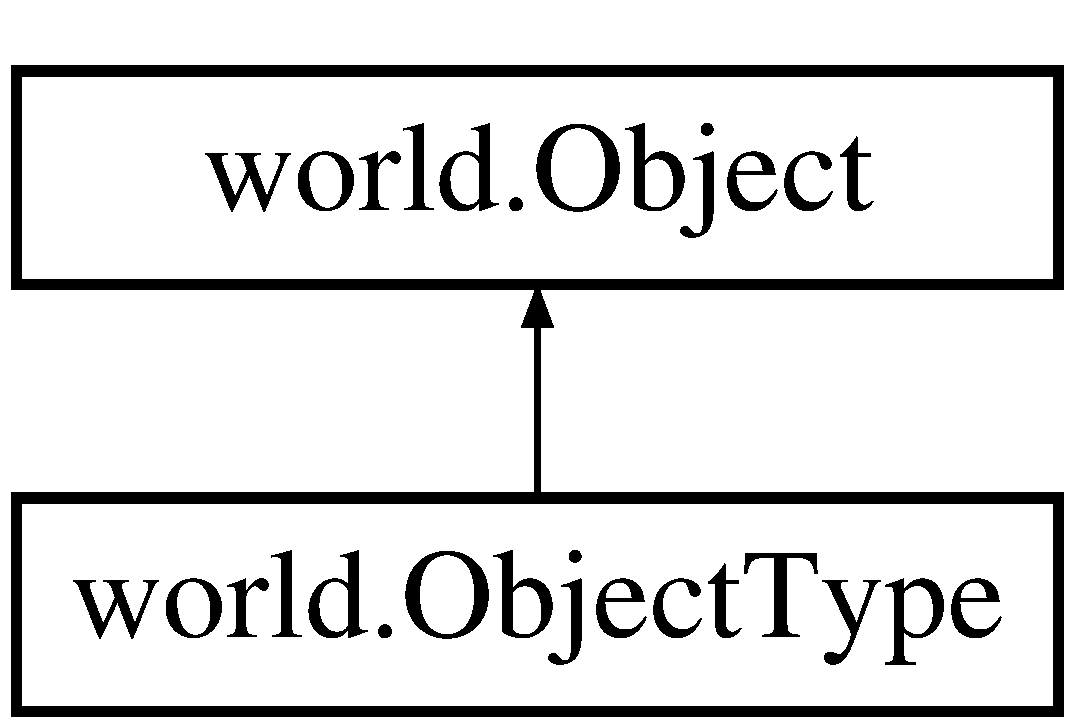
\includegraphics[height=2.000000cm]{classworld_1_1_object_type}
\end{center}
\end{figure}
\subsection*{\-Public \-Member \-Functions}
\begin{DoxyCompactItemize}
\item 
\hypertarget{classworld_1_1_object_type_a8e22b69e8867f70d768f1c29b5d67299}{def {\bfseries \-\_\-\-\_\-init\-\_\-\-\_\-}}\label{classworld_1_1_object_type_a8e22b69e8867f70d768f1c29b5d67299}

\item 
def \hyperlink{classworld_1_1_object_type_aec3659e529c2f58cc8ec05a759811015}{create}
\end{DoxyCompactItemize}
\subsection*{\-Public \-Attributes}
\begin{DoxyCompactItemize}
\item 
\hypertarget{classworld_1_1_object_type_ae9880fda72c8950d1b1b070efa72279e}{{\bfseries type}}\label{classworld_1_1_object_type_ae9880fda72c8950d1b1b070efa72279e}

\end{DoxyCompactItemize}


\subsection{\-Detailed \-Description}
\begin{DoxyVerb}Les types d'objets (au sens informatique) \end{DoxyVerb}
 

\subsection{\-Member \-Function \-Documentation}
\hypertarget{classworld_1_1_object_type_aec3659e529c2f58cc8ec05a759811015}{\index{world\-::\-Object\-Type@{world\-::\-Object\-Type}!create@{create}}
\index{create@{create}!world::ObjectType@{world\-::\-Object\-Type}}
\subsubsection[{create}]{\setlength{\rightskip}{0pt plus 5cm}def {\bf world.\-Object\-Type.\-create} (
\begin{DoxyParamCaption}
\item[{}]{self}
\end{DoxyParamCaption}
)}}\label{classworld_1_1_object_type_aec3659e529c2f58cc8ec05a759811015}
\begin{DoxyVerb}Instanticiation d'un objet à partir du type \end{DoxyVerb}
 

\-The documentation for this class was generated from the following file\-:\begin{DoxyCompactItemize}
\item 
src/shared/world.\-py\end{DoxyCompactItemize}

\hypertarget{classorders_1_1_order}{\section{orders.\-Order \-Class \-Reference}
\label{classorders_1_1_order}\index{orders.\-Order@{orders.\-Order}}
}
\subsection*{\-Public \-Member \-Functions}
\begin{DoxyCompactItemize}
\item 
\hypertarget{classorders_1_1_order_a9edb54cb84082a08a74e530fd1e76b1b}{def {\bfseries \-\_\-\-\_\-init\-\_\-\-\_\-}}\label{classorders_1_1_order_a9edb54cb84082a08a74e530fd1e76b1b}

\item 
\hypertarget{classorders_1_1_order_a59845607c6c2fa3acd7de4a2ce77dcc9}{def {\bfseries \-\_\-\-\_\-getattr\-\_\-\-\_\-}}\label{classorders_1_1_order_a59845607c6c2fa3acd7de4a2ce77dcc9}

\item 
\hypertarget{classorders_1_1_order_a2e56120bbdf2113577a02c4363c62962}{def {\bfseries \-\_\-\-\_\-setattr\-\_\-\-\_\-}}\label{classorders_1_1_order_a2e56120bbdf2113577a02c4363c62962}

\item 
def \hyperlink{classorders_1_1_order_a078dacfd495f75c137de77d841befb70}{copy}
\item 
def \hyperlink{classorders_1_1_order_aa008e119a00013ed8483f6a4ea7245d9}{set\-Type}
\item 
def \hyperlink{classorders_1_1_order_a780c0dbab2da2360364f90ab01eb844f}{load}
\item 
def \hyperlink{classorders_1_1_order_ac2672b32c4cbe4666d7d1cdf71cd54b7}{to\-Bytes}
\item 
def \hyperlink{classorders_1_1_order_a66e727b5ba70f44495cd2a15e079c9eb}{from\-Bytes}
\end{DoxyCompactItemize}
\subsection*{\-Public \-Attributes}
\begin{DoxyCompactItemize}
\item 
\hypertarget{classorders_1_1_order_afb4003458342b2aeebb67c8bc89afefa}{{\bfseries type}}\label{classorders_1_1_order_afb4003458342b2aeebb67c8bc89afefa}

\item 
\hypertarget{classorders_1_1_order_a04e5f09b80a685f731d291e0de2a61db}{{\bfseries args}}\label{classorders_1_1_order_a04e5f09b80a685f731d291e0de2a61db}

\end{DoxyCompactItemize}
\subsection*{\-Static \-Public \-Attributes}
\begin{DoxyCompactItemize}
\item 
\hypertarget{classorders_1_1_order_a8c362161ec6b78b5a5a04cf63ba79a0d}{list {\bfseries params} = \mbox{[}\-None\mbox{]}}\label{classorders_1_1_order_a8c362161ec6b78b5a5a04cf63ba79a0d}

\end{DoxyCompactItemize}


\subsection{\-Detailed \-Description}
\begin{DoxyVerb}A change to be done on the world\end{DoxyVerb}
 

\subsection{\-Member \-Function \-Documentation}
\hypertarget{classorders_1_1_order_a078dacfd495f75c137de77d841befb70}{\index{orders\-::\-Order@{orders\-::\-Order}!copy@{copy}}
\index{copy@{copy}!orders::Order@{orders\-::\-Order}}
\subsubsection[{copy}]{\setlength{\rightskip}{0pt plus 5cm}def {\bf orders.\-Order.\-copy} (
\begin{DoxyParamCaption}
\item[{}]{self}
\end{DoxyParamCaption}
)}}\label{classorders_1_1_order_a078dacfd495f75c137de77d841befb70}
\begin{DoxyVerb}Copy the object from class Order \end{DoxyVerb}
 \hypertarget{classorders_1_1_order_a66e727b5ba70f44495cd2a15e079c9eb}{\index{orders\-::\-Order@{orders\-::\-Order}!from\-Bytes@{from\-Bytes}}
\index{from\-Bytes@{from\-Bytes}!orders::Order@{orders\-::\-Order}}
\subsubsection[{from\-Bytes}]{\setlength{\rightskip}{0pt plus 5cm}def {\bf orders.\-Order.\-from\-Bytes} (
\begin{DoxyParamCaption}
\item[{}]{self, }
\item[{}]{byt}
\end{DoxyParamCaption}
)}}\label{classorders_1_1_order_a66e727b5ba70f44495cd2a15e079c9eb}
\begin{DoxyVerb}Retrieve order from network bytes \end{DoxyVerb}
 \hypertarget{classorders_1_1_order_a780c0dbab2da2360364f90ab01eb844f}{\index{orders\-::\-Order@{orders\-::\-Order}!load@{load}}
\index{load@{load}!orders::Order@{orders\-::\-Order}}
\subsubsection[{load}]{\setlength{\rightskip}{0pt plus 5cm}def {\bf orders.\-Order.\-load} (
\begin{DoxyParamCaption}
\item[{}]{self, }
\item[{}]{dat, }
\item[{}]{named}
\end{DoxyParamCaption}
)}}\label{classorders_1_1_order_a780c0dbab2da2360364f90ab01eb844f}
\begin{DoxyVerb}Initialise the order with an Xml structure \end{DoxyVerb}
 \hypertarget{classorders_1_1_order_aa008e119a00013ed8483f6a4ea7245d9}{\index{orders\-::\-Order@{orders\-::\-Order}!set\-Type@{set\-Type}}
\index{set\-Type@{set\-Type}!orders::Order@{orders\-::\-Order}}
\subsubsection[{set\-Type}]{\setlength{\rightskip}{0pt plus 5cm}def {\bf orders.\-Order.\-set\-Type} (
\begin{DoxyParamCaption}
\item[{}]{self, }
\item[{}]{typ}
\end{DoxyParamCaption}
)}}\label{classorders_1_1_order_aa008e119a00013ed8483f6a4ea7245d9}
\begin{DoxyVerb}Initialise args according to the given type \end{DoxyVerb}
 \hypertarget{classorders_1_1_order_ac2672b32c4cbe4666d7d1cdf71cd54b7}{\index{orders\-::\-Order@{orders\-::\-Order}!to\-Bytes@{to\-Bytes}}
\index{to\-Bytes@{to\-Bytes}!orders::Order@{orders\-::\-Order}}
\subsubsection[{to\-Bytes}]{\setlength{\rightskip}{0pt plus 5cm}def {\bf orders.\-Order.\-to\-Bytes} (
\begin{DoxyParamCaption}
\item[{}]{self}
\end{DoxyParamCaption}
)}}\label{classorders_1_1_order_ac2672b32c4cbe4666d7d1cdf71cd54b7}
\begin{DoxyVerb}Bytes to send the order on the network \end{DoxyVerb}
 

\-The documentation for this class was generated from the following file\-:\begin{DoxyCompactItemize}
\item 
src/shared/orders.\-py\end{DoxyCompactItemize}

\hypertarget{classorders_1_1_order_dispatcher}{\section{orders.\-Order\-Dispatcher \-Class \-Reference}
\label{classorders_1_1_order_dispatcher}\index{orders.\-Order\-Dispatcher@{orders.\-Order\-Dispatcher}}
}
\subsection*{\-Public \-Member \-Functions}
\begin{DoxyCompactItemize}
\item 
\hypertarget{classorders_1_1_order_dispatcher_ae49ccd75a98bf4d03734acabc60a8191}{def {\bfseries \-\_\-\-\_\-init\-\_\-\-\_\-}}\label{classorders_1_1_order_dispatcher_ae49ccd75a98bf4d03734acabc60a8191}

\item 
def \hyperlink{classorders_1_1_order_dispatcher_ad7ce3b5e93f23334280236d7b3f65c01}{treat}
\end{DoxyCompactItemize}
\subsection*{\-Public \-Attributes}
\begin{DoxyCompactItemize}
\item 
\hypertarget{classorders_1_1_order_dispatcher_a3e8a2d43b1b5849af6d2556d6bca5b18}{{\bfseries world}}\label{classorders_1_1_order_dispatcher_a3e8a2d43b1b5849af6d2556d6bca5b18}

\item 
\hypertarget{classorders_1_1_order_dispatcher_a46638f289946e25105aa54056c792324}{{\bfseries handle}}\label{classorders_1_1_order_dispatcher_a46638f289946e25105aa54056c792324}

\item 
\hypertarget{classorders_1_1_order_dispatcher_a753b3b377c0103eb3130eca0e792e75d}{{\bfseries timer}}\label{classorders_1_1_order_dispatcher_a753b3b377c0103eb3130eca0e792e75d}

\end{DoxyCompactItemize}


\subsection{\-Detailed \-Description}
\begin{DoxyVerb}Traite les ordres pour le client ou le serveur \end{DoxyVerb}
 

\subsection{\-Member \-Function \-Documentation}
\hypertarget{classorders_1_1_order_dispatcher_ad7ce3b5e93f23334280236d7b3f65c01}{\index{orders\-::\-Order\-Dispatcher@{orders\-::\-Order\-Dispatcher}!treat@{treat}}
\index{treat@{treat}!orders::OrderDispatcher@{orders\-::\-Order\-Dispatcher}}
\subsubsection[{treat}]{\setlength{\rightskip}{0pt plus 5cm}def {\bf orders.\-Order\-Dispatcher.\-treat} (
\begin{DoxyParamCaption}
\item[{}]{self, }
\item[{}]{emitter, }
\item[{}]{order}
\end{DoxyParamCaption}
)}}\label{classorders_1_1_order_dispatcher_ad7ce3b5e93f23334280236d7b3f65c01}
\begin{DoxyVerb}Traite un ordre et renvoie l'éventuel ordre à retransmettre \end{DoxyVerb}
 

\-The documentation for this class was generated from the following file\-:\begin{DoxyCompactItemize}
\item 
src/shared/orders.\-py\end{DoxyCompactItemize}

\hypertarget{classtools_1_1_perf}{\section{tools.\-Perf \-Class \-Reference}
\label{classtools_1_1_perf}\index{tools.\-Perf@{tools.\-Perf}}
}
\subsection*{\-Public \-Member \-Functions}
\begin{DoxyCompactItemize}
\item 
\hypertarget{classtools_1_1_perf_a2a9656142836ccd440cd478b8c556f36}{def {\bfseries \-\_\-\-\_\-init\-\_\-\-\_\-}}\label{classtools_1_1_perf_a2a9656142836ccd440cd478b8c556f36}

\item 
def \hyperlink{classtools_1_1_perf_a89caef783edbd23d7cf8d1856f56b615}{tic}
\item 
def \hyperlink{classtools_1_1_perf_aad55535c6c6e0fa197ad789aab0588dc}{toc}
\item 
def \hyperlink{classtools_1_1_perf_a8a3420997340d5ddfee55b5db1c11a07}{show}
\end{DoxyCompactItemize}
\subsection*{\-Public \-Attributes}
\begin{DoxyCompactItemize}
\item 
\hypertarget{classtools_1_1_perf_ab807cd43fffe3ba57431f338b1b507b3}{{\bfseries num}}\label{classtools_1_1_perf_ab807cd43fffe3ba57431f338b1b507b3}

\item 
\hypertarget{classtools_1_1_perf_a93aee8a86289a6fce942b2fcb3297cde}{{\bfseries avg}}\label{classtools_1_1_perf_a93aee8a86289a6fce942b2fcb3297cde}

\item 
\hypertarget{classtools_1_1_perf_ae08d1949f5e4f74dab5792b61e40f922}{{\bfseries min}}\label{classtools_1_1_perf_ae08d1949f5e4f74dab5792b61e40f922}

\item 
\hypertarget{classtools_1_1_perf_ae5a7677a5d3930bb576fb8a76d978725}{{\bfseries max}}\label{classtools_1_1_perf_ae5a7677a5d3930bb576fb8a76d978725}

\item 
\hypertarget{classtools_1_1_perf_a08f6383b13c04a93a5ad0cdc196efecd}{{\bfseries t}}\label{classtools_1_1_perf_a08f6383b13c04a93a5ad0cdc196efecd}

\end{DoxyCompactItemize}


\subsection{\-Detailed \-Description}
\begin{DoxyVerb}Times a piece of code \end{DoxyVerb}
 

\subsection{\-Member \-Function \-Documentation}
\hypertarget{classtools_1_1_perf_a8a3420997340d5ddfee55b5db1c11a07}{\index{tools\-::\-Perf@{tools\-::\-Perf}!show@{show}}
\index{show@{show}!tools::Perf@{tools\-::\-Perf}}
\subsubsection[{show}]{\setlength{\rightskip}{0pt plus 5cm}def {\bf tools.\-Perf.\-show} (
\begin{DoxyParamCaption}
\item[{}]{self}
\end{DoxyParamCaption}
)}}\label{classtools_1_1_perf_a8a3420997340d5ddfee55b5db1c11a07}
\begin{DoxyVerb}Print stats \end{DoxyVerb}
 \hypertarget{classtools_1_1_perf_a89caef783edbd23d7cf8d1856f56b615}{\index{tools\-::\-Perf@{tools\-::\-Perf}!tic@{tic}}
\index{tic@{tic}!tools::Perf@{tools\-::\-Perf}}
\subsubsection[{tic}]{\setlength{\rightskip}{0pt plus 5cm}def {\bf tools.\-Perf.\-tic} (
\begin{DoxyParamCaption}
\item[{}]{self}
\end{DoxyParamCaption}
)}}\label{classtools_1_1_perf_a89caef783edbd23d7cf8d1856f56b615}
\begin{DoxyVerb}To be run before the timed function \end{DoxyVerb}
 \hypertarget{classtools_1_1_perf_aad55535c6c6e0fa197ad789aab0588dc}{\index{tools\-::\-Perf@{tools\-::\-Perf}!toc@{toc}}
\index{toc@{toc}!tools::Perf@{tools\-::\-Perf}}
\subsubsection[{toc}]{\setlength{\rightskip}{0pt plus 5cm}def {\bf tools.\-Perf.\-toc} (
\begin{DoxyParamCaption}
\item[{}]{self}
\end{DoxyParamCaption}
)}}\label{classtools_1_1_perf_aad55535c6c6e0fa197ad789aab0588dc}
\begin{DoxyVerb}To be run after the timed function \end{DoxyVerb}
 

\-The documentation for this class was generated from the following file\-:\begin{DoxyCompactItemize}
\item 
src/shared/tools.\-py\end{DoxyCompactItemize}

\hypertarget{classplugins_1_1plugin_1_1_plugin}{\section{plugins.\-plugin.\-Plugin \-Class \-Reference}
\label{classplugins_1_1plugin_1_1_plugin}\index{plugins.\-plugin.\-Plugin@{plugins.\-plugin.\-Plugin}}
}
\-Inheritance diagram for plugins.\-plugin.\-Plugin\-:\begin{figure}[H]
\begin{center}
\leavevmode
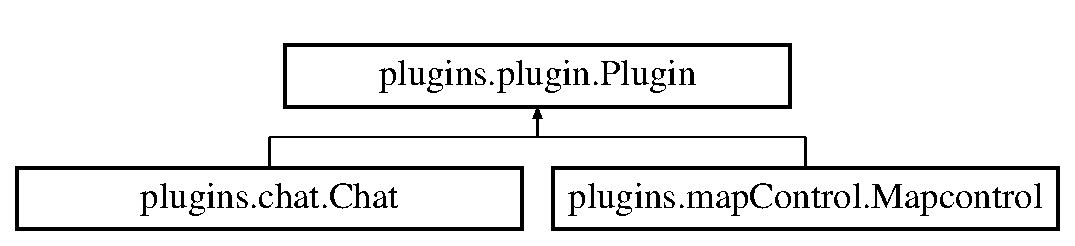
\includegraphics[height=2.000000cm]{classplugins_1_1plugin_1_1_plugin}
\end{center}
\end{figure}
\subsection*{\-Public \-Member \-Functions}
\begin{DoxyCompactItemize}
\item 
\hypertarget{classplugins_1_1plugin_1_1_plugin_a66f5c840ac03b9b724fb9734669abdfb}{def {\bfseries \-\_\-\-\_\-init\-\_\-\-\_\-}}\label{classplugins_1_1plugin_1_1_plugin_a66f5c840ac03b9b724fb9734669abdfb}

\item 
def \hyperlink{classplugins_1_1plugin_1_1_plugin_aac06ba69452a3dac4e5950116a34d3ac}{server\-Message}
\item 
def \hyperlink{classplugins_1_1plugin_1_1_plugin_a9647791e5ba3150f5fd82bb359a43d11}{client\-Message}
\item 
\hypertarget{classplugins_1_1plugin_1_1_plugin_a977c6c1cb7ea7cbb54667f8264da135c}{def {\bfseries send}}\label{classplugins_1_1plugin_1_1_plugin_a977c6c1cb7ea7cbb54667f8264da135c}

\item 
\hypertarget{classplugins_1_1plugin_1_1_plugin_a030ec3807307c32b09dc91b8f4d3ede9}{def {\bfseries broadcast}}\label{classplugins_1_1plugin_1_1_plugin_a030ec3807307c32b09dc91b8f4d3ede9}

\end{DoxyCompactItemize}
\subsection*{\-Public \-Attributes}
\begin{DoxyCompactItemize}
\item 
\hypertarget{classplugins_1_1plugin_1_1_plugin_a27cac3b42754566db40b9cb0109648b4}{{\bfseries engine}}\label{classplugins_1_1plugin_1_1_plugin_a27cac3b42754566db40b9cb0109648b4}

\item 
\hypertarget{classplugins_1_1plugin_1_1_plugin_aac6f72b7299d7727ad2e851fc49d7adb}{{\bfseries ui}}\label{classplugins_1_1plugin_1_1_plugin_aac6f72b7299d7727ad2e851fc49d7adb}

\end{DoxyCompactItemize}
\subsection*{\-Static \-Public \-Attributes}
\begin{DoxyCompactItemize}
\item 
\hypertarget{classplugins_1_1plugin_1_1_plugin_a6610c8a6ee2aa96841e955601a71048b}{{\bfseries \-C\-B\-T\-I\-M\-E} = \-None}\label{classplugins_1_1plugin_1_1_plugin_a6610c8a6ee2aa96841e955601a71048b}

\item 
\hypertarget{classplugins_1_1plugin_1_1_plugin_aef32d2e4903ca91abc7a719b7e6ce561}{string {\bfseries \-M\-S\-G\-I\-D} = \char`\"{}\char`\"{}}\label{classplugins_1_1plugin_1_1_plugin_aef32d2e4903ca91abc7a719b7e6ce561}

\end{DoxyCompactItemize}


\subsection{\-Detailed \-Description}
\begin{DoxyVerb}To write a network plugin, subclass this and reimplement attributes
and virtual methods\end{DoxyVerb}
 

\subsection{\-Member \-Function \-Documentation}
\hypertarget{classplugins_1_1plugin_1_1_plugin_a9647791e5ba3150f5fd82bb359a43d11}{\index{plugins\-::plugin\-::\-Plugin@{plugins\-::plugin\-::\-Plugin}!client\-Message@{client\-Message}}
\index{client\-Message@{client\-Message}!plugins::plugin::Plugin@{plugins\-::plugin\-::\-Plugin}}
\subsubsection[{client\-Message}]{\setlength{\rightskip}{0pt plus 5cm}def {\bf plugins.\-plugin.\-Plugin.\-client\-Message} (
\begin{DoxyParamCaption}
\item[{}]{self, }
\item[{}]{msg}
\end{DoxyParamCaption}
)}}\label{classplugins_1_1plugin_1_1_plugin_a9647791e5ba3150f5fd82bb359a43d11}
\begin{DoxyVerb}called then bytes msg are sent to the client \end{DoxyVerb}
 

\-Reimplemented in \hyperlink{classplugins_1_1chat_1_1_chat_ad241689aeb8b03c689248ffb18584d40}{plugins.\-chat.\-Chat}.

\hypertarget{classplugins_1_1plugin_1_1_plugin_aac06ba69452a3dac4e5950116a34d3ac}{\index{plugins\-::plugin\-::\-Plugin@{plugins\-::plugin\-::\-Plugin}!server\-Message@{server\-Message}}
\index{server\-Message@{server\-Message}!plugins::plugin::Plugin@{plugins\-::plugin\-::\-Plugin}}
\subsubsection[{server\-Message}]{\setlength{\rightskip}{0pt plus 5cm}def {\bf plugins.\-plugin.\-Plugin.\-server\-Message} (
\begin{DoxyParamCaption}
\item[{}]{self, }
\item[{}]{msg}
\end{DoxyParamCaption}
)}}\label{classplugins_1_1plugin_1_1_plugin_aac06ba69452a3dac4e5950116a34d3ac}
\begin{DoxyVerb}called then bytes msg are sent to the server \end{DoxyVerb}
 

\-Reimplemented in \hyperlink{classplugins_1_1chat_1_1_chat_af8546a2537aee9bf99e09007649e2320}{plugins.\-chat.\-Chat}.



\-The documentation for this class was generated from the following file\-:\begin{DoxyCompactItemize}
\item 
src/plugins/plugin.\-py\end{DoxyCompactItemize}

\hypertarget{classplugins_1_1plugin_1_1_pygame_plugin}{\section{plugins.\-plugin.\-Pygame\-Plugin \-Class \-Reference}
\label{classplugins_1_1plugin_1_1_pygame_plugin}\index{plugins.\-plugin.\-Pygame\-Plugin@{plugins.\-plugin.\-Pygame\-Plugin}}
}
\subsection*{\-Public \-Member \-Functions}
\begin{DoxyCompactItemize}
\item 
\hypertarget{classplugins_1_1plugin_1_1_pygame_plugin_a883e10c5bea4b72d2674b5b3a0715a6f}{def {\bfseries \-\_\-\-\_\-init\-\_\-\-\_\-}}\label{classplugins_1_1plugin_1_1_pygame_plugin_a883e10c5bea4b72d2674b5b3a0715a6f}

\item 
def \hyperlink{classplugins_1_1plugin_1_1_pygame_plugin_ad1780000a3ee47c8c239612ff4fa9d74}{handle\-Event}
\item 
def \hyperlink{classplugins_1_1plugin_1_1_pygame_plugin_a459513cbe6410dd4743c54adad4416de}{draw}
\item 
def \hyperlink{classplugins_1_1plugin_1_1_pygame_plugin_a9cc79e76b41cff27bbdc6a4e23c5febc}{update}
\end{DoxyCompactItemize}
\subsection*{\-Public \-Attributes}
\begin{DoxyCompactItemize}
\item 
\hypertarget{classplugins_1_1plugin_1_1_pygame_plugin_add14cfc41c87ebbe8a6023c4e3c2d3aa}{{\bfseries net\-Plugin}}\label{classplugins_1_1plugin_1_1_pygame_plugin_add14cfc41c87ebbe8a6023c4e3c2d3aa}

\item 
\hypertarget{classplugins_1_1plugin_1_1_pygame_plugin_af23330154421938d139ad55579b1257b}{{\bfseries image}}\label{classplugins_1_1plugin_1_1_pygame_plugin_af23330154421938d139ad55579b1257b}

\item 
\hypertarget{classplugins_1_1plugin_1_1_pygame_plugin_abeeaffe2ad0e6269f2bc3af25d00117a}{{\bfseries rect}}\label{classplugins_1_1plugin_1_1_pygame_plugin_abeeaffe2ad0e6269f2bc3af25d00117a}

\end{DoxyCompactItemize}


\subsection{\-Detailed \-Description}
\begin{DoxyVerb}Subclass this to write a pygame plugin, which is a layer that should
    be drawn on screen over the map\end{DoxyVerb}
 

\subsection{\-Member \-Function \-Documentation}
\hypertarget{classplugins_1_1plugin_1_1_pygame_plugin_a459513cbe6410dd4743c54adad4416de}{\index{plugins\-::plugin\-::\-Pygame\-Plugin@{plugins\-::plugin\-::\-Pygame\-Plugin}!draw@{draw}}
\index{draw@{draw}!plugins::plugin::PygamePlugin@{plugins\-::plugin\-::\-Pygame\-Plugin}}
\subsubsection[{draw}]{\setlength{\rightskip}{0pt plus 5cm}def {\bf plugins.\-plugin.\-Pygame\-Plugin.\-draw} (
\begin{DoxyParamCaption}
\item[{}]{self}
\end{DoxyParamCaption}
)}}\label{classplugins_1_1plugin_1_1_pygame_plugin_a459513cbe6410dd4743c54adad4416de}
\begin{DoxyVerb}creates/updates the Surface to blit \end{DoxyVerb}
 \hypertarget{classplugins_1_1plugin_1_1_pygame_plugin_ad1780000a3ee47c8c239612ff4fa9d74}{\index{plugins\-::plugin\-::\-Pygame\-Plugin@{plugins\-::plugin\-::\-Pygame\-Plugin}!handle\-Event@{handle\-Event}}
\index{handle\-Event@{handle\-Event}!plugins::plugin::PygamePlugin@{plugins\-::plugin\-::\-Pygame\-Plugin}}
\subsubsection[{handle\-Event}]{\setlength{\rightskip}{0pt plus 5cm}def {\bf plugins.\-plugin.\-Pygame\-Plugin.\-handle\-Event} (
\begin{DoxyParamCaption}
\item[{}]{self, }
\item[{}]{event}
\end{DoxyParamCaption}
)}}\label{classplugins_1_1plugin_1_1_pygame_plugin_ad1780000a3ee47c8c239612ff4fa9d74}
\begin{DoxyVerb}return True if the key has been used \end{DoxyVerb}
 \hypertarget{classplugins_1_1plugin_1_1_pygame_plugin_a9cc79e76b41cff27bbdc6a4e23c5febc}{\index{plugins\-::plugin\-::\-Pygame\-Plugin@{plugins\-::plugin\-::\-Pygame\-Plugin}!update@{update}}
\index{update@{update}!plugins::plugin::PygamePlugin@{plugins\-::plugin\-::\-Pygame\-Plugin}}
\subsubsection[{update}]{\setlength{\rightskip}{0pt plus 5cm}def {\bf plugins.\-plugin.\-Pygame\-Plugin.\-update} (
\begin{DoxyParamCaption}
\item[{}]{self}
\end{DoxyParamCaption}
)}}\label{classplugins_1_1plugin_1_1_pygame_plugin_a9cc79e76b41cff27bbdc6a4e23c5febc}
\begin{DoxyVerb}do updates \end{DoxyVerb}
 

\-The documentation for this class was generated from the following file\-:\begin{DoxyCompactItemize}
\item 
src/plugins/plugin.\-py\end{DoxyCompactItemize}

\hypertarget{classinterface_1_1cache_1_1_scaled_cache}{\section{interface.\-cache.\-Scaled\-Cache \-Class \-Reference}
\label{classinterface_1_1cache_1_1_scaled_cache}\index{interface.\-cache.\-Scaled\-Cache@{interface.\-cache.\-Scaled\-Cache}}
}
\-Inheritance diagram for interface.\-cache.\-Scaled\-Cache\-:\begin{figure}[H]
\begin{center}
\leavevmode
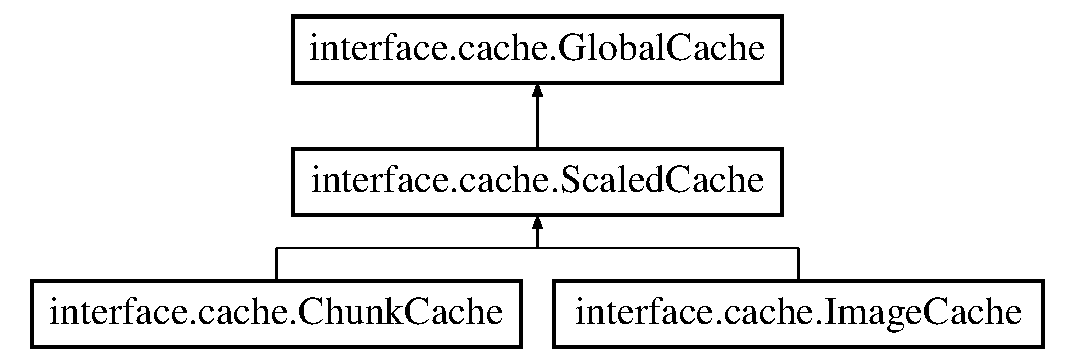
\includegraphics[height=3.000000cm]{classinterface_1_1cache_1_1_scaled_cache}
\end{center}
\end{figure}
\subsection*{\-Public \-Member \-Functions}
\begin{DoxyCompactItemize}
\item 
\hypertarget{classinterface_1_1cache_1_1_scaled_cache_ab7f44dd02e1f049ee4ceea02da0e70e0}{def {\bfseries add\-\_\-scaled}}\label{classinterface_1_1cache_1_1_scaled_cache_ab7f44dd02e1f049ee4ceea02da0e70e0}

\item 
\hypertarget{classinterface_1_1cache_1_1_scaled_cache_a66a6408691eb1620de6ed7f6b8fc4e77}{def {\bfseries remove}}\label{classinterface_1_1cache_1_1_scaled_cache_a66a6408691eb1620de6ed7f6b8fc4e77}

\item 
\hypertarget{classinterface_1_1cache_1_1_scaled_cache_a0a2104e6521edb1641c4db70a5326278}{def {\bfseries get\-\_\-elt}}\label{classinterface_1_1cache_1_1_scaled_cache_a0a2104e6521edb1641c4db70a5326278}

\item 
\hypertarget{classinterface_1_1cache_1_1_scaled_cache_a49373b4d908d75102df24d95cfb8778d}{def {\bfseries free\-\_\-cache}}\label{classinterface_1_1cache_1_1_scaled_cache_a49373b4d908d75102df24d95cfb8778d}

\end{DoxyCompactItemize}


\subsection{\-Detailed \-Description}
\begin{DoxyVerb}
Each entry in the cache is an array of the same object at
different scales.
\end{DoxyVerb}
 

\-The documentation for this class was generated from the following file\-:\begin{DoxyCompactItemize}
\item 
src/interface/cache.\-py\end{DoxyCompactItemize}

\hypertarget{classserver_1_1_server}{\section{server.\-Server \-Class \-Reference}
\label{classserver_1_1_server}\index{server.\-Server@{server.\-Server}}
}
\subsection*{\-Public \-Member \-Functions}
\begin{DoxyCompactItemize}
\item 
\hypertarget{classserver_1_1_server_a423441de73b670b0f72d1cd83e6e9b96}{def {\bfseries \-\_\-\-\_\-init\-\_\-\-\_\-}}\label{classserver_1_1_server_a423441de73b670b0f72d1cd83e6e9b96}

\item 
\hypertarget{classserver_1_1_server_ac80c3a945398c3c941f5d0820c823b88}{def {\bfseries \-\_\-\-\_\-del\-\_\-\-\_\-}}\label{classserver_1_1_server_ac80c3a945398c3c941f5d0820c823b88}

\item 
def \hyperlink{classserver_1_1_server_a9b3fa0cb53b66ff0f4b5cab8257e1f97}{run}
\item 
def \hyperlink{classserver_1_1_server_a00234be60c5d9f6fcb3dd40ce8b7eaf0}{main}
\item 
def \hyperlink{classserver_1_1_server_a27e7213342658fc1f0a689647963be9a}{handle\-Event}
\item 
def \hyperlink{classserver_1_1_server_a96a93fb7b3ede34e861cba3952cd85e2}{plugin\-Handle}
\end{DoxyCompactItemize}
\subsection*{\-Public \-Attributes}
\begin{DoxyCompactItemize}
\item 
\hypertarget{classserver_1_1_server_aa66c4b037c112c4777cdc3d0b021bf0a}{{\bfseries loop}}\label{classserver_1_1_server_aa66c4b037c112c4777cdc3d0b021bf0a}

\item 
\hypertarget{classserver_1_1_server_a7c744a2e1c5d36f4e41ee16b15eddec0}{{\bfseries net}}\label{classserver_1_1_server_a7c744a2e1c5d36f4e41ee16b15eddec0}

\item 
\hypertarget{classserver_1_1_server_afb24f0dc3380595ca5fa1e3720eddf91}{{\bfseries world}}\label{classserver_1_1_server_afb24f0dc3380595ca5fa1e3720eddf91}

\item 
\hypertarget{classserver_1_1_server_ac18f6cc461c554eb4f5975bae585beb1}{{\bfseries actions}}\label{classserver_1_1_server_ac18f6cc461c554eb4f5975bae585beb1}

\item 
\hypertarget{classserver_1_1_server_a173029dc00b8683b075d277c668617b9}{{\bfseries plugins}}\label{classserver_1_1_server_a173029dc00b8683b075d277c668617b9}

\item 
\hypertarget{classserver_1_1_server_a648310f189b51c6fe5b0c9b925c638ae}{{\bfseries timer}}\label{classserver_1_1_server_a648310f189b51c6fe5b0c9b925c638ae}

\item 
\hypertarget{classserver_1_1_server_a7bef2487ef91bc73d3c7686ddd42daf2}{{\bfseries order\-Dispatcher}}\label{classserver_1_1_server_a7bef2487ef91bc73d3c7686ddd42daf2}

\item 
\hypertarget{classserver_1_1_server_a59d51ebb6587b77ef52a1f2533a0c7a8}{{\bfseries events}}\label{classserver_1_1_server_a59d51ebb6587b77ef52a1f2533a0c7a8}

\item 
\hypertarget{classserver_1_1_server_a7e6fa74117ab619b24b38bedb698b26e}{{\bfseries pause}}\label{classserver_1_1_server_a7e6fa74117ab619b24b38bedb698b26e}

\end{DoxyCompactItemize}


\subsection{\-Detailed \-Description}
\begin{DoxyVerb}Main class of the server process, gathering network, world, actions and timer \end{DoxyVerb}
 

\subsection{\-Member \-Function \-Documentation}
\hypertarget{classserver_1_1_server_a27e7213342658fc1f0a689647963be9a}{\index{server\-::\-Server@{server\-::\-Server}!handle\-Event@{handle\-Event}}
\index{handle\-Event@{handle\-Event}!server::Server@{server\-::\-Server}}
\subsubsection[{handle\-Event}]{\setlength{\rightskip}{0pt plus 5cm}def {\bf server.\-Server.\-handle\-Event} (
\begin{DoxyParamCaption}
\item[{}]{self, }
\item[{}]{emitter, }
\item[{}]{event}
\end{DoxyParamCaption}
)}}\label{classserver_1_1_server_a27e7213342658fc1f0a689647963be9a}
\begin{DoxyVerb}Add a event to the queue \end{DoxyVerb}
 \hypertarget{classserver_1_1_server_a00234be60c5d9f6fcb3dd40ce8b7eaf0}{\index{server\-::\-Server@{server\-::\-Server}!main@{main}}
\index{main@{main}!server::Server@{server\-::\-Server}}
\subsubsection[{main}]{\setlength{\rightskip}{0pt plus 5cm}def {\bf server.\-Server.\-main} (
\begin{DoxyParamCaption}
\item[{}]{self}
\end{DoxyParamCaption}
)}}\label{classserver_1_1_server_a00234be60c5d9f6fcb3dd40ce8b7eaf0}
\begin{DoxyVerb}Init stuff, read events and ask for treatment \end{DoxyVerb}
 \hypertarget{classserver_1_1_server_a96a93fb7b3ede34e861cba3952cd85e2}{\index{server\-::\-Server@{server\-::\-Server}!plugin\-Handle@{plugin\-Handle}}
\index{plugin\-Handle@{plugin\-Handle}!server::Server@{server\-::\-Server}}
\subsubsection[{plugin\-Handle}]{\setlength{\rightskip}{0pt plus 5cm}def {\bf server.\-Server.\-plugin\-Handle} (
\begin{DoxyParamCaption}
\item[{}]{self, }
\item[{}]{msg}
\end{DoxyParamCaption}
)}}\label{classserver_1_1_server_a96a93fb7b3ede34e861cba3952cd85e2}
\begin{DoxyVerb}Search for plugins that want to handle the message \end{DoxyVerb}
 \hypertarget{classserver_1_1_server_a9b3fa0cb53b66ff0f4b5cab8257e1f97}{\index{server\-::\-Server@{server\-::\-Server}!run@{run}}
\index{run@{run}!server::Server@{server\-::\-Server}}
\subsubsection[{run}]{\setlength{\rightskip}{0pt plus 5cm}def {\bf server.\-Server.\-run} (
\begin{DoxyParamCaption}
\item[{}]{self}
\end{DoxyParamCaption}
)}}\label{classserver_1_1_server_a9b3fa0cb53b66ff0f4b5cab8257e1f97}
\begin{DoxyVerb}Launch tasks \end{DoxyVerb}
 

\-The documentation for this class was generated from the following file\-:\begin{DoxyCompactItemize}
\item 
src/server.\-py\end{DoxyCompactItemize}

\hypertarget{classnetwork_1_1_server_connection}{\section{network.\-Server\-Connection \-Class \-Reference}
\label{classnetwork_1_1_server_connection}\index{network.\-Server\-Connection@{network.\-Server\-Connection}}
}
\subsection*{\-Public \-Member \-Functions}
\begin{DoxyCompactItemize}
\item 
\hypertarget{classnetwork_1_1_server_connection_a1818bbe7e2a0d4729ba76fafeecf90a0}{def {\bfseries \-\_\-\-\_\-init\-\_\-\-\_\-}}\label{classnetwork_1_1_server_connection_a1818bbe7e2a0d4729ba76fafeecf90a0}

\item 
def \hyperlink{classnetwork_1_1_server_connection_ab84090c243e9153e6fc06d545c4a8968}{run}
\item 
\hypertarget{classnetwork_1_1_server_connection_a6bcc6b09e3359518d050488c2269b28b}{def {\bfseries send}}\label{classnetwork_1_1_server_connection_a6bcc6b09e3359518d050488c2269b28b}

\item 
\hypertarget{classnetwork_1_1_server_connection_a113c3428c88f0a5b37bcc71d5252eaa2}{def {\bfseries end}}\label{classnetwork_1_1_server_connection_a113c3428c88f0a5b37bcc71d5252eaa2}

\end{DoxyCompactItemize}
\subsection*{\-Public \-Attributes}
\begin{DoxyCompactItemize}
\item 
\hypertarget{classnetwork_1_1_server_connection_af5084b55a486eebc40ea6c24cbfcc337}{{\bfseries reader}}\label{classnetwork_1_1_server_connection_af5084b55a486eebc40ea6c24cbfcc337}

\item 
\hypertarget{classnetwork_1_1_server_connection_aef54f357fd46b50f54006b999a2f54ec}{{\bfseries writer}}\label{classnetwork_1_1_server_connection_aef54f357fd46b50f54006b999a2f54ec}

\item 
\hypertarget{classnetwork_1_1_server_connection_ac05b83aca4479be68d65d260a6cb9882}{{\bfseries handle}}\label{classnetwork_1_1_server_connection_ac05b83aca4479be68d65d260a6cb9882}

\item 
\hypertarget{classnetwork_1_1_server_connection_ad94a2f09f0d783fb74bcfd69891280c7}{{\bfseries plugin\-Handle}}\label{classnetwork_1_1_server_connection_ad94a2f09f0d783fb74bcfd69891280c7}

\item 
\hypertarget{classnetwork_1_1_server_connection_ac8e3086a76124ee9449998f99c95adf1}{{\bfseries entity}}\label{classnetwork_1_1_server_connection_ac8e3086a76124ee9449998f99c95adf1}

\item 
\hypertarget{classnetwork_1_1_server_connection_a3b7560c8cd5b2d3bfd5a66a644297d60}{{\bfseries server}}\label{classnetwork_1_1_server_connection_a3b7560c8cd5b2d3bfd5a66a644297d60}

\end{DoxyCompactItemize}


\subsection{\-Detailed \-Description}
\begin{DoxyVerb}
This thread manages the communications with one particular client (one
thread is created by client).
\end{DoxyVerb}
 

\subsection{\-Member \-Function \-Documentation}
\hypertarget{classnetwork_1_1_server_connection_ab84090c243e9153e6fc06d545c4a8968}{\index{network\-::\-Server\-Connection@{network\-::\-Server\-Connection}!run@{run}}
\index{run@{run}!network::ServerConnection@{network\-::\-Server\-Connection}}
\subsubsection[{run}]{\setlength{\rightskip}{0pt plus 5cm}def {\bf network.\-Server\-Connection.\-run} (
\begin{DoxyParamCaption}
\item[{}]{self}
\end{DoxyParamCaption}
)}}\label{classnetwork_1_1_server_connection_ab84090c243e9153e6fc06d545c4a8968}
\begin{DoxyVerb}
Wait for messages from the client and handle them immediately.
\end{DoxyVerb}
 

\-The documentation for this class was generated from the following file\-:\begin{DoxyCompactItemize}
\item 
src/shared/network.\-py\end{DoxyCompactItemize}

\hypertarget{classtest_1_1_test__register_interactions}{\section{test.\-Test\-\_\-register\-Interactions \-Class \-Reference}
\label{classtest_1_1_test__register_interactions}\index{test.\-Test\-\_\-register\-Interactions@{test.\-Test\-\_\-register\-Interactions}}
}
\subsection*{\-Public \-Member \-Functions}
\begin{DoxyCompactItemize}
\item 
\hypertarget{classtest_1_1_test__register_interactions_a323022aeef3c33601dfa21f181fa58e9}{def {\bfseries test\-\_\-}}\label{classtest_1_1_test__register_interactions_a323022aeef3c33601dfa21f181fa58e9}

\end{DoxyCompactItemize}


\-The documentation for this class was generated from the following file\-:\begin{DoxyCompactItemize}
\item 
src/test.\-py\end{DoxyCompactItemize}

\hypertarget{classtest_1_1_test_action}{\section{test.\-Test\-Action \-Class \-Reference}
\label{classtest_1_1_test_action}\index{test.\-Test\-Action@{test.\-Test\-Action}}
}
\subsection*{\-Public \-Member \-Functions}
\begin{DoxyCompactItemize}
\item 
\hypertarget{classtest_1_1_test_action_aa865e367d501fed852e019430edfb0c8}{def {\bfseries test\-\_\-}}\label{classtest_1_1_test_action_aa865e367d501fed852e019430edfb0c8}

\end{DoxyCompactItemize}


\-The documentation for this class was generated from the following file\-:\begin{DoxyCompactItemize}
\item 
src/test.\-py\end{DoxyCompactItemize}

\hypertarget{classtest_1_1_test_client}{\section{test.\-Test\-Client \-Class \-Reference}
\label{classtest_1_1_test_client}\index{test.\-Test\-Client@{test.\-Test\-Client}}
}
\subsection*{\-Public \-Member \-Functions}
\begin{DoxyCompactItemize}
\item 
\hypertarget{classtest_1_1_test_client_ac755b41364bcbd58ef8539796cfacbeb}{def {\bfseries test\-\_\-}}\label{classtest_1_1_test_client_ac755b41364bcbd58ef8539796cfacbeb}

\end{DoxyCompactItemize}


\-The documentation for this class was generated from the following file\-:\begin{DoxyCompactItemize}
\item 
src/test.\-py\end{DoxyCompactItemize}

\hypertarget{classtest_1_1_test_curses}{\section{test.\-Test\-Curses \-Class \-Reference}
\label{classtest_1_1_test_curses}\index{test.\-Test\-Curses@{test.\-Test\-Curses}}
}
\subsection*{\-Public \-Member \-Functions}
\begin{DoxyCompactItemize}
\item 
\hypertarget{classtest_1_1_test_curses_a6da36996c09fd0d3154e942a7e0cd505}{def {\bfseries test\-\_\-}}\label{classtest_1_1_test_curses_a6da36996c09fd0d3154e942a7e0cd505}

\end{DoxyCompactItemize}


\-The documentation for this class was generated from the following file\-:\begin{DoxyCompactItemize}
\item 
src/test.\-py\end{DoxyCompactItemize}

\hypertarget{classtest_1_1_test_interface}{\section{test.\-Test\-Interface \-Class \-Reference}
\label{classtest_1_1_test_interface}\index{test.\-Test\-Interface@{test.\-Test\-Interface}}
}
\subsection*{\-Public \-Member \-Functions}
\begin{DoxyCompactItemize}
\item 
\hypertarget{classtest_1_1_test_interface_a654b56179796283bd5127dc36a66a9c1}{def {\bfseries test\-\_\-}}\label{classtest_1_1_test_interface_a654b56179796283bd5127dc36a66a9c1}

\end{DoxyCompactItemize}


\-The documentation for this class was generated from the following file\-:\begin{DoxyCompactItemize}
\item 
src/test.\-py\end{DoxyCompactItemize}

\hypertarget{classtest_1_1_test_network_client}{\section{test.\-Test\-Network\-Client \-Class \-Reference}
\label{classtest_1_1_test_network_client}\index{test.\-Test\-Network\-Client@{test.\-Test\-Network\-Client}}
}
\subsection*{\-Public \-Member \-Functions}
\begin{DoxyCompactItemize}
\item 
\hypertarget{classtest_1_1_test_network_client_a78d057e96ed185dbaac67a9e67a29d44}{def {\bfseries test\-\_\-}}\label{classtest_1_1_test_network_client_a78d057e96ed185dbaac67a9e67a29d44}

\end{DoxyCompactItemize}


\-The documentation for this class was generated from the following file\-:\begin{DoxyCompactItemize}
\item 
src/test.\-py\end{DoxyCompactItemize}

\hypertarget{classtest_1_1_test_network_server}{\section{test.\-Test\-Network\-Server \-Class \-Reference}
\label{classtest_1_1_test_network_server}\index{test.\-Test\-Network\-Server@{test.\-Test\-Network\-Server}}
}
\subsection*{\-Public \-Member \-Functions}
\begin{DoxyCompactItemize}
\item 
\hypertarget{classtest_1_1_test_network_server_a391ecf52930ae668e5e3b7d78ccf9324}{def {\bfseries test\-\_\-}}\label{classtest_1_1_test_network_server_a391ecf52930ae668e5e3b7d78ccf9324}

\end{DoxyCompactItemize}


\-The documentation for this class was generated from the following file\-:\begin{DoxyCompactItemize}
\item 
src/test.\-py\end{DoxyCompactItemize}

\hypertarget{classtest_1_1_test_order}{\section{test.\-Test\-Order \-Class \-Reference}
\label{classtest_1_1_test_order}\index{test.\-Test\-Order@{test.\-Test\-Order}}
}
\subsection*{\-Public \-Member \-Functions}
\begin{DoxyCompactItemize}
\item 
\hypertarget{classtest_1_1_test_order_a3d56be2de858998e14172a9dd6ff5fe4}{def {\bfseries test\-\_\-}}\label{classtest_1_1_test_order_a3d56be2de858998e14172a9dd6ff5fe4}

\end{DoxyCompactItemize}
\subsection*{\-Static \-Public \-Attributes}
\begin{DoxyCompactItemize}
\item 
\hypertarget{classtest_1_1_test_order_a2935afd2f861642116f4076c9c260de6}{tuple {\bfseries o} = \-Order()}\label{classtest_1_1_test_order_a2935afd2f861642116f4076c9c260de6}

\item 
\hypertarget{classtest_1_1_test_order_ab1f28e7686e62878c934ef911aae8ba4}{tuple {\bfseries b} = o.\-to\-Bytes()}\label{classtest_1_1_test_order_ab1f28e7686e62878c934ef911aae8ba4}

\item 
\hypertarget{classtest_1_1_test_order_a8b82b9b5a8a4f5b385348774c3ca364e}{tuple {\bfseries oo} = \-Order()}\label{classtest_1_1_test_order_a8b82b9b5a8a4f5b385348774c3ca364e}

\end{DoxyCompactItemize}


\-The documentation for this class was generated from the following file\-:\begin{DoxyCompactItemize}
\item 
src/test.\-py\end{DoxyCompactItemize}

\hypertarget{classtest_1_1_test_order_dispatcher}{\section{test.\-Test\-Order\-Dispatcher \-Class \-Reference}
\label{classtest_1_1_test_order_dispatcher}\index{test.\-Test\-Order\-Dispatcher@{test.\-Test\-Order\-Dispatcher}}
}
\subsection*{\-Public \-Member \-Functions}
\begin{DoxyCompactItemize}
\item 
\hypertarget{classtest_1_1_test_order_dispatcher_a2ea286ce39d6d156cae967e70ae79c38}{def {\bfseries test\-\_\-}}\label{classtest_1_1_test_order_dispatcher_a2ea286ce39d6d156cae967e70ae79c38}

\end{DoxyCompactItemize}


\-The documentation for this class was generated from the following file\-:\begin{DoxyCompactItemize}
\item 
src/test.\-py\end{DoxyCompactItemize}

\hypertarget{classtest_1_1_test_perf}{\section{test.\-Test\-Perf \-Class \-Reference}
\label{classtest_1_1_test_perf}\index{test.\-Test\-Perf@{test.\-Test\-Perf}}
}
\subsection*{\-Public \-Member \-Functions}
\begin{DoxyCompactItemize}
\item 
\hypertarget{classtest_1_1_test_perf_ae83d1066d3b9b32d1560c23e11b9b3e0}{def {\bfseries test\-\_\-}}\label{classtest_1_1_test_perf_ae83d1066d3b9b32d1560c23e11b9b3e0}

\end{DoxyCompactItemize}


\-The documentation for this class was generated from the following file\-:\begin{DoxyCompactItemize}
\item 
src/test.\-py\end{DoxyCompactItemize}

\hypertarget{classtest_1_1_testread_xml}{\section{test.\-Testread\-Xml \-Class \-Reference}
\label{classtest_1_1_testread_xml}\index{test.\-Testread\-Xml@{test.\-Testread\-Xml}}
}
\subsection*{\-Public \-Member \-Functions}
\begin{DoxyCompactItemize}
\item 
\hypertarget{classtest_1_1_testread_xml_a15f08f56300089e6c9e4e5fe533179cf}{def {\bfseries test\-\_\-}}\label{classtest_1_1_testread_xml_a15f08f56300089e6c9e4e5fe533179cf}

\end{DoxyCompactItemize}


\-The documentation for this class was generated from the following file\-:\begin{DoxyCompactItemize}
\item 
src/test.\-py\end{DoxyCompactItemize}

\hypertarget{classtest_1_1_test_server_connection}{\section{test.\-Test\-Server\-Connection \-Class \-Reference}
\label{classtest_1_1_test_server_connection}\index{test.\-Test\-Server\-Connection@{test.\-Test\-Server\-Connection}}
}
\subsection*{\-Public \-Member \-Functions}
\begin{DoxyCompactItemize}
\item 
\hypertarget{classtest_1_1_test_server_connection_ac62e9eb7418ae13d1ba768da3f490d63}{def {\bfseries test\-\_\-}}\label{classtest_1_1_test_server_connection_ac62e9eb7418ae13d1ba768da3f490d63}

\end{DoxyCompactItemize}


\-The documentation for this class was generated from the following file\-:\begin{DoxyCompactItemize}
\item 
src/test.\-py\end{DoxyCompactItemize}

\hypertarget{classtest_1_1_test_string_methods}{\section{test.\-Test\-String\-Methods \-Class \-Reference}
\label{classtest_1_1_test_string_methods}\index{test.\-Test\-String\-Methods@{test.\-Test\-String\-Methods}}
}


\-Inherits \-Test\-Case.

\subsection*{\-Public \-Member \-Functions}
\begin{DoxyCompactItemize}
\item 
\hypertarget{classtest_1_1_test_string_methods_a22eca18953d31e7aa44ec2c3c76cbfe4}{def {\bfseries test\-\_\-upper}}\label{classtest_1_1_test_string_methods_a22eca18953d31e7aa44ec2c3c76cbfe4}

\item 
\hypertarget{classtest_1_1_test_string_methods_a476b22edee75ca28bcfc3537dcecd7a1}{def {\bfseries test\-\_\-isupper}}\label{classtest_1_1_test_string_methods_a476b22edee75ca28bcfc3537dcecd7a1}

\item 
\hypertarget{classtest_1_1_test_string_methods_a35decc36a9e989f8021574f3b6aa26b2}{def {\bfseries test\-\_\-split}}\label{classtest_1_1_test_string_methods_a35decc36a9e989f8021574f3b6aa26b2}

\end{DoxyCompactItemize}


\-The documentation for this class was generated from the following file\-:\begin{DoxyCompactItemize}
\item 
src/test.\-py\end{DoxyCompactItemize}

\hypertarget{classtest_1_1_test_timer}{\section{test.\-Test\-Timer \-Class \-Reference}
\label{classtest_1_1_test_timer}\index{test.\-Test\-Timer@{test.\-Test\-Timer}}
}
\subsection*{\-Public \-Member \-Functions}
\begin{DoxyCompactItemize}
\item 
\hypertarget{classtest_1_1_test_timer_a0b652b39096ce9aef3be80dc3d5fa72f}{def {\bfseries test\-\_\-}}\label{classtest_1_1_test_timer_a0b652b39096ce9aef3be80dc3d5fa72f}

\end{DoxyCompactItemize}


\-The documentation for this class was generated from the following file\-:\begin{DoxyCompactItemize}
\item 
src/test.\-py\end{DoxyCompactItemize}

\hypertarget{classtools_1_1_timer}{\section{tools.\-Timer \-Class \-Reference}
\label{classtools_1_1_timer}\index{tools.\-Timer@{tools.\-Timer}}
}
\subsection*{\-Public \-Member \-Functions}
\begin{DoxyCompactItemize}
\item 
\hypertarget{classtools_1_1_timer_aa8eb0f7637ab77b3558633a24267ec12}{def {\bfseries \-\_\-\-\_\-init\-\_\-\-\_\-}}\label{classtools_1_1_timer_aa8eb0f7637ab77b3558633a24267ec12}

\item 
def \hyperlink{classtools_1_1_timer_a5f2a146060a63948098337885132c3cf}{add}
\item 
def \hyperlink{classtools_1_1_timer_ae3470afe22648a6bc6cd7104bb3fc4e2}{run}
\end{DoxyCompactItemize}
\subsection*{\-Public \-Attributes}
\begin{DoxyCompactItemize}
\item 
\hypertarget{classtools_1_1_timer_a4979bfdbf6635ea450ecefd1f3db623a}{{\bfseries dt}}\label{classtools_1_1_timer_a4979bfdbf6635ea450ecefd1f3db623a}

\item 
\hypertarget{classtools_1_1_timer_a893d0a9a5e7d031b0f1af5efc5743cc8}{{\bfseries step}}\label{classtools_1_1_timer_a893d0a9a5e7d031b0f1af5efc5743cc8}

\item 
\hypertarget{classtools_1_1_timer_a3023e0d71d6badac61bc599dcfd1eb8c}{{\bfseries heap}}\label{classtools_1_1_timer_a3023e0d71d6badac61bc599dcfd1eb8c}

\item 
\hypertarget{classtools_1_1_timer_ad498ee353df48ed8e3e018e0ed61bea4}{{\bfseries pause}}\label{classtools_1_1_timer_ad498ee353df48ed8e3e018e0ed61bea4}

\item 
\hypertarget{classtools_1_1_timer_a3b500aad25a782ff35fdc0a0c08b92ed}{{\bfseries count}}\label{classtools_1_1_timer_a3b500aad25a782ff35fdc0a0c08b92ed}

\item 
\hypertarget{classtools_1_1_timer_a57e5a80add7f6e9cbebefae90b737e04}{{\bfseries time}}\label{classtools_1_1_timer_a57e5a80add7f6e9cbebefae90b737e04}

\end{DoxyCompactItemize}


\subsection{\-Detailed \-Description}
\begin{DoxyVerb}Trigger differed couroutine calls \end{DoxyVerb}
 

\subsection{\-Member \-Function \-Documentation}
\hypertarget{classtools_1_1_timer_a5f2a146060a63948098337885132c3cf}{\index{tools\-::\-Timer@{tools\-::\-Timer}!add@{add}}
\index{add@{add}!tools::Timer@{tools\-::\-Timer}}
\subsubsection[{add}]{\setlength{\rightskip}{0pt plus 5cm}def {\bf tools.\-Timer.\-add} (
\begin{DoxyParamCaption}
\item[{}]{self, }
\item[{}]{time, }
\item[{}]{func, }
\item[{}]{args}
\end{DoxyParamCaption}
)}}\label{classtools_1_1_timer_a5f2a146060a63948098337885132c3cf}
\begin{DoxyVerb}Write the function func call with arguments args \end{DoxyVerb}
 \hypertarget{classtools_1_1_timer_ae3470afe22648a6bc6cd7104bb3fc4e2}{\index{tools\-::\-Timer@{tools\-::\-Timer}!run@{run}}
\index{run@{run}!tools::Timer@{tools\-::\-Timer}}
\subsubsection[{run}]{\setlength{\rightskip}{0pt plus 5cm}def {\bf tools.\-Timer.\-run} (
\begin{DoxyParamCaption}
\item[{}]{self}
\end{DoxyParamCaption}
)}}\label{classtools_1_1_timer_ae3470afe22648a6bc6cd7104bb3fc4e2}
\begin{DoxyVerb}Working task \end{DoxyVerb}
 

\-The documentation for this class was generated from the following file\-:\begin{DoxyCompactItemize}
\item 
src/shared/tools.\-py\end{DoxyCompactItemize}

\hypertarget{classinterface_1_1utils_1_1_walkable_graph}{\section{interface.\-utils.\-Walkable\-Graph \-Class \-Reference}
\label{classinterface_1_1utils_1_1_walkable_graph}\index{interface.\-utils.\-Walkable\-Graph@{interface.\-utils.\-Walkable\-Graph}}
}
\subsection*{\-Public \-Member \-Functions}
\begin{DoxyCompactItemize}
\item 
def \hyperlink{classinterface_1_1utils_1_1_walkable_graph_ab278b45be983e6f0a0867e92f874bf9e}{\-\_\-\-\_\-init\-\_\-\-\_\-}
\item 
def \hyperlink{classinterface_1_1utils_1_1_walkable_graph_a7767f3578dbbe420d17c3fd276b0db89}{get\-\_\-neighbors}
\item 
def \hyperlink{classinterface_1_1utils_1_1_walkable_graph_af3bf5d30e760b5086ef700465009d226}{dist}
\item 
def \hyperlink{classinterface_1_1utils_1_1_walkable_graph_aa0a83b900040d019fae13289cf70521a}{get\-\_\-path}
\end{DoxyCompactItemize}
\subsection*{\-Public \-Attributes}
\begin{DoxyCompactItemize}
\item 
\hypertarget{classinterface_1_1utils_1_1_walkable_graph_a51e03368d01089484beeb703ce69104e}{{\bfseries walkables}}\label{classinterface_1_1utils_1_1_walkable_graph_a51e03368d01089484beeb703ce69104e}

\end{DoxyCompactItemize}


\subsection{\-Constructor \& \-Destructor \-Documentation}
\hypertarget{classinterface_1_1utils_1_1_walkable_graph_ab278b45be983e6f0a0867e92f874bf9e}{\index{interface\-::utils\-::\-Walkable\-Graph@{interface\-::utils\-::\-Walkable\-Graph}!\-\_\-\-\_\-init\-\_\-\-\_\-@{\-\_\-\-\_\-init\-\_\-\-\_\-}}
\index{\-\_\-\-\_\-init\-\_\-\-\_\-@{\-\_\-\-\_\-init\-\_\-\-\_\-}!interface::utils::WalkableGraph@{interface\-::utils\-::\-Walkable\-Graph}}
\subsubsection[{\-\_\-\-\_\-init\-\_\-\-\_\-}]{\setlength{\rightskip}{0pt plus 5cm}def {\bf interface.\-utils.\-Walkable\-Graph.\-\_\-\-\_\-init\-\_\-\-\_\-} (
\begin{DoxyParamCaption}
\item[{}]{self, }
\item[{}]{walkables}
\end{DoxyParamCaption}
)}}\label{classinterface_1_1utils_1_1_walkable_graph_ab278b45be983e6f0a0867e92f874bf9e}
\begin{DoxyVerb}
Walkables is a bit array representing cells that can be crossed
during a move
\end{DoxyVerb}
 

\subsection{\-Member \-Function \-Documentation}
\hypertarget{classinterface_1_1utils_1_1_walkable_graph_af3bf5d30e760b5086ef700465009d226}{\index{interface\-::utils\-::\-Walkable\-Graph@{interface\-::utils\-::\-Walkable\-Graph}!dist@{dist}}
\index{dist@{dist}!interface::utils::WalkableGraph@{interface\-::utils\-::\-Walkable\-Graph}}
\subsubsection[{dist}]{\setlength{\rightskip}{0pt plus 5cm}def {\bf interface.\-utils.\-Walkable\-Graph.\-dist} (
\begin{DoxyParamCaption}
\item[{}]{self, }
\item[{}]{u, }
\item[{}]{v}
\end{DoxyParamCaption}
)}}\label{classinterface_1_1utils_1_1_walkable_graph_af3bf5d30e760b5086ef700465009d226}
\begin{DoxyVerb}Return distance between two nodes on the grid \end{DoxyVerb}
 \hypertarget{classinterface_1_1utils_1_1_walkable_graph_a7767f3578dbbe420d17c3fd276b0db89}{\index{interface\-::utils\-::\-Walkable\-Graph@{interface\-::utils\-::\-Walkable\-Graph}!get\-\_\-neighbors@{get\-\_\-neighbors}}
\index{get\-\_\-neighbors@{get\-\_\-neighbors}!interface::utils::WalkableGraph@{interface\-::utils\-::\-Walkable\-Graph}}
\subsubsection[{get\-\_\-neighbors}]{\setlength{\rightskip}{0pt plus 5cm}def {\bf interface.\-utils.\-Walkable\-Graph.\-get\-\_\-neighbors} (
\begin{DoxyParamCaption}
\item[{}]{self, }
\item[{}]{index}
\end{DoxyParamCaption}
)}}\label{classinterface_1_1utils_1_1_walkable_graph_a7767f3578dbbe420d17c3fd276b0db89}
\begin{DoxyVerb}
Return accessible cells around index, with a cost value depending
on the direction of the move.
\end{DoxyVerb}
 \hypertarget{classinterface_1_1utils_1_1_walkable_graph_aa0a83b900040d019fae13289cf70521a}{\index{interface\-::utils\-::\-Walkable\-Graph@{interface\-::utils\-::\-Walkable\-Graph}!get\-\_\-path@{get\-\_\-path}}
\index{get\-\_\-path@{get\-\_\-path}!interface::utils::WalkableGraph@{interface\-::utils\-::\-Walkable\-Graph}}
\subsubsection[{get\-\_\-path}]{\setlength{\rightskip}{0pt plus 5cm}def {\bf interface.\-utils.\-Walkable\-Graph.\-get\-\_\-path} (
\begin{DoxyParamCaption}
\item[{}]{self, }
\item[{}]{source, }
\item[{}]{dest}
\end{DoxyParamCaption}
)}}\label{classinterface_1_1utils_1_1_walkable_graph_aa0a83b900040d019fae13289cf70521a}
\begin{DoxyVerb}A* algorithm on the current graph \end{DoxyVerb}
 

\-The documentation for this class was generated from the following file\-:\begin{DoxyCompactItemize}
\item 
src/interface/utils.\-py\end{DoxyCompactItemize}

\hypertarget{classworld_1_1_world}{\section{world.\-World \-Class \-Reference}
\label{classworld_1_1_world}\index{world.\-World@{world.\-World}}
}
\subsection*{\-Public \-Member \-Functions}
\begin{DoxyCompactItemize}
\item 
\hypertarget{classworld_1_1_world_a4351253668240be9d3a0d5bc2f1aa18f}{def {\bfseries \-\_\-\-\_\-init\-\_\-\-\_\-}}\label{classworld_1_1_world_a4351253668240be9d3a0d5bc2f1aa18f}

\end{DoxyCompactItemize}
\subsection*{\-Public \-Attributes}
\begin{DoxyCompactItemize}
\item 
\hypertarget{classworld_1_1_world_ae5d81046b959889536deca60b2df94a4}{{\bfseries maps}}\label{classworld_1_1_world_ae5d81046b959889536deca60b2df94a4}

\item 
\hypertarget{classworld_1_1_world_ae2c39feccf4fcd06f11f8398e42505a4}{{\bfseries entities}}\label{classworld_1_1_world_ae2c39feccf4fcd06f11f8398e42505a4}

\item 
\hypertarget{classworld_1_1_world_a144e6d2a815857b12be4cd2bf4ac2c44}{{\bfseries objects}}\label{classworld_1_1_world_a144e6d2a815857b12be4cd2bf4ac2c44}

\end{DoxyCompactItemize}


\subsection{\-Detailed \-Description}
\begin{DoxyVerb}\end{DoxyVerb}
 

\-The documentation for this class was generated from the following file\-:\begin{DoxyCompactItemize}
\item 
src/shared/world.\-py\end{DoxyCompactItemize}

\hypertarget{classinterface_1_1print_world_1_1_world_viewer}{\section{interface.\-print\-World.\-World\-Viewer \-Class \-Reference}
\label{classinterface_1_1print_world_1_1_world_viewer}\index{interface.\-print\-World.\-World\-Viewer@{interface.\-print\-World.\-World\-Viewer}}
}
\-Inheritance diagram for interface.\-print\-World.\-World\-Viewer\-:\begin{figure}[H]
\begin{center}
\leavevmode
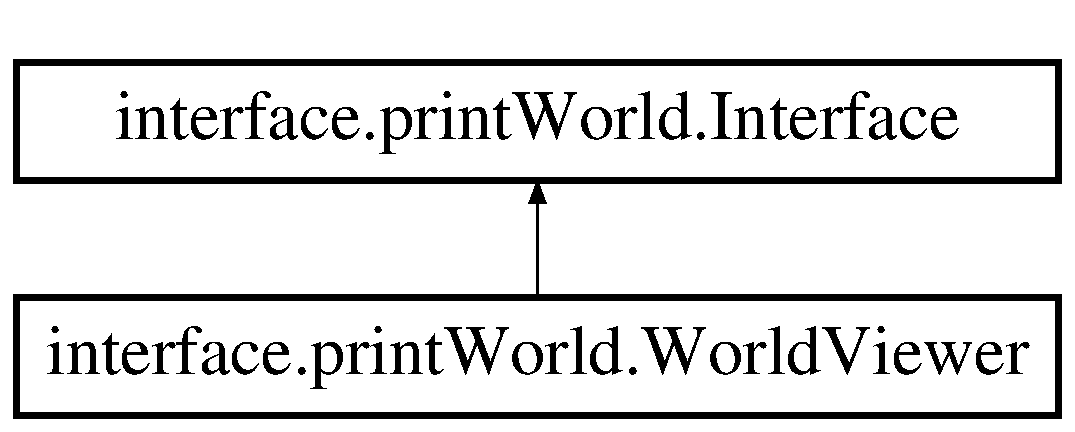
\includegraphics[height=2.000000cm]{classinterface_1_1print_world_1_1_world_viewer}
\end{center}
\end{figure}
\subsection*{\-Public \-Member \-Functions}
\begin{DoxyCompactItemize}
\item 
def \hyperlink{classinterface_1_1print_world_1_1_world_viewer_a29df52052f8f790a3e1308d102210186}{\-\_\-\-\_\-init\-\_\-\-\_\-}
\item 
def \hyperlink{classinterface_1_1print_world_1_1_world_viewer_adada0d39c5e5f93da8d50722a04e7b92}{get\-\_\-event}
\item 
def \hyperlink{classinterface_1_1print_world_1_1_world_viewer_a060018a5214380bf5e539a8742a34201}{end}
\item 
\hypertarget{classinterface_1_1print_world_1_1_world_viewer_a6fe7808a1e9b09c56d1838ff36a3f8f2}{def {\bfseries set\-\_\-perso}}\label{classinterface_1_1print_world_1_1_world_viewer_a6fe7808a1e9b09c56d1838ff36a3f8f2}

\item 
def \hyperlink{classinterface_1_1print_world_1_1_world_viewer_a9cc6b5953ef4bfcfca631b6a94554cac}{update}
\item 
def \hyperlink{classinterface_1_1print_world_1_1_world_viewer_a16f9b59c20fd0e54125da6d4cbcc373e}{render}
\item 
def \hyperlink{classinterface_1_1print_world_1_1_world_viewer_a29cbfc89a67d46a31ca889cf481d5e2f}{move}
\item 
def \hyperlink{classinterface_1_1print_world_1_1_world_viewer_a14fd62fb5ee0b63011028e1e84cf19f4}{propagate\-\_\-trigger}
\end{DoxyCompactItemize}
\subsection*{\-Public \-Attributes}
\begin{DoxyCompactItemize}
\item 
\hypertarget{classinterface_1_1print_world_1_1_world_viewer_a2d27f4fd1714ebe00461c66a273e6ac6}{{\bfseries screen\-\_\-size}}\label{classinterface_1_1print_world_1_1_world_viewer_a2d27f4fd1714ebe00461c66a273e6ac6}

\item 
\hypertarget{classinterface_1_1print_world_1_1_world_viewer_a2d31a07969ff3371cffeb6f8919a34a9}{{\bfseries current\-\_\-map}}\label{classinterface_1_1print_world_1_1_world_viewer_a2d31a07969ff3371cffeb6f8919a34a9}

\item 
\hypertarget{classinterface_1_1print_world_1_1_world_viewer_a0b5d398be53a8a24243dfd58905d55db}{{\bfseries entities}}\label{classinterface_1_1print_world_1_1_world_viewer_a0b5d398be53a8a24243dfd58905d55db}

\item 
\hypertarget{classinterface_1_1print_world_1_1_world_viewer_a242edaf710e3c9c3fae3d7e7f90888c4}{{\bfseries perso}}\label{classinterface_1_1print_world_1_1_world_viewer_a242edaf710e3c9c3fae3d7e7f90888c4}

\end{DoxyCompactItemize}


\subsection{\-Constructor \& \-Destructor \-Documentation}
\hypertarget{classinterface_1_1print_world_1_1_world_viewer_a29df52052f8f790a3e1308d102210186}{\index{interface\-::print\-World\-::\-World\-Viewer@{interface\-::print\-World\-::\-World\-Viewer}!\-\_\-\-\_\-init\-\_\-\-\_\-@{\-\_\-\-\_\-init\-\_\-\-\_\-}}
\index{\-\_\-\-\_\-init\-\_\-\-\_\-@{\-\_\-\-\_\-init\-\_\-\-\_\-}!interface::printWorld::WorldViewer@{interface\-::print\-World\-::\-World\-Viewer}}
\subsubsection[{\-\_\-\-\_\-init\-\_\-\-\_\-}]{\setlength{\rightskip}{0pt plus 5cm}def {\bf interface.\-print\-World.\-World\-Viewer.\-\_\-\-\_\-init\-\_\-\-\_\-} (
\begin{DoxyParamCaption}
\item[{}]{self, }
\item[{}]{w}
\end{DoxyParamCaption}
)}}\label{classinterface_1_1print_world_1_1_world_viewer_a29df52052f8f790a3e1308d102210186}
\begin{DoxyVerb}Initialize the pygame Interface \end{DoxyVerb}
 

\subsection{\-Member \-Function \-Documentation}
\hypertarget{classinterface_1_1print_world_1_1_world_viewer_a060018a5214380bf5e539a8742a34201}{\index{interface\-::print\-World\-::\-World\-Viewer@{interface\-::print\-World\-::\-World\-Viewer}!end@{end}}
\index{end@{end}!interface::printWorld::WorldViewer@{interface\-::print\-World\-::\-World\-Viewer}}
\subsubsection[{end}]{\setlength{\rightskip}{0pt plus 5cm}def {\bf interface.\-print\-World.\-World\-Viewer.\-end} (
\begin{DoxyParamCaption}
\item[{}]{self}
\end{DoxyParamCaption}
)}}\label{classinterface_1_1print_world_1_1_world_viewer_a060018a5214380bf5e539a8742a34201}
\begin{DoxyVerb}End the display \end{DoxyVerb}
 \hypertarget{classinterface_1_1print_world_1_1_world_viewer_adada0d39c5e5f93da8d50722a04e7b92}{\index{interface\-::print\-World\-::\-World\-Viewer@{interface\-::print\-World\-::\-World\-Viewer}!get\-\_\-event@{get\-\_\-event}}
\index{get\-\_\-event@{get\-\_\-event}!interface::printWorld::WorldViewer@{interface\-::print\-World\-::\-World\-Viewer}}
\subsubsection[{get\-\_\-event}]{\setlength{\rightskip}{0pt plus 5cm}def {\bf interface.\-print\-World.\-World\-Viewer.\-get\-\_\-event} (
\begin{DoxyParamCaption}
\item[{}]{self}
\end{DoxyParamCaption}
)}}\label{classinterface_1_1print_world_1_1_world_viewer_adada0d39c5e5f93da8d50722a04e7b92}
\begin{DoxyVerb}Return current pygame events stack \end{DoxyVerb}
 \hypertarget{classinterface_1_1print_world_1_1_world_viewer_a29cbfc89a67d46a31ca889cf481d5e2f}{\index{interface\-::print\-World\-::\-World\-Viewer@{interface\-::print\-World\-::\-World\-Viewer}!move@{move}}
\index{move@{move}!interface::printWorld::WorldViewer@{interface\-::print\-World\-::\-World\-Viewer}}
\subsubsection[{move}]{\setlength{\rightskip}{0pt plus 5cm}def {\bf interface.\-print\-World.\-World\-Viewer.\-move} (
\begin{DoxyParamCaption}
\item[{}]{self, }
\item[{}]{dx, }
\item[{}]{dy}
\end{DoxyParamCaption}
)}}\label{classinterface_1_1print_world_1_1_world_viewer_a29cbfc89a67d46a31ca889cf481d5e2f}
\begin{DoxyVerb}Move the current map by dx,dy, return the rectangle of
    modifications\end{DoxyVerb}
 \hypertarget{classinterface_1_1print_world_1_1_world_viewer_a14fd62fb5ee0b63011028e1e84cf19f4}{\index{interface\-::print\-World\-::\-World\-Viewer@{interface\-::print\-World\-::\-World\-Viewer}!propagate\-\_\-trigger@{propagate\-\_\-trigger}}
\index{propagate\-\_\-trigger@{propagate\-\_\-trigger}!interface::printWorld::WorldViewer@{interface\-::print\-World\-::\-World\-Viewer}}
\subsubsection[{propagate\-\_\-trigger}]{\setlength{\rightskip}{0pt plus 5cm}def {\bf interface.\-print\-World.\-World\-Viewer.\-propagate\-\_\-trigger} (
\begin{DoxyParamCaption}
\item[{}]{self, }
\item[{}]{event}
\end{DoxyParamCaption}
)}}\label{classinterface_1_1print_world_1_1_world_viewer_a14fd62fb5ee0b63011028e1e84cf19f4}
\begin{DoxyVerb}Propagate event to next objects in the arborescence, here its the
    current map \end{DoxyVerb}
 \hypertarget{classinterface_1_1print_world_1_1_world_viewer_a16f9b59c20fd0e54125da6d4cbcc373e}{\index{interface\-::print\-World\-::\-World\-Viewer@{interface\-::print\-World\-::\-World\-Viewer}!render@{render}}
\index{render@{render}!interface::printWorld::WorldViewer@{interface\-::print\-World\-::\-World\-Viewer}}
\subsubsection[{render}]{\setlength{\rightskip}{0pt plus 5cm}def {\bf interface.\-print\-World.\-World\-Viewer.\-render} (
\begin{DoxyParamCaption}
\item[{}]{self}
\end{DoxyParamCaption}
)}}\label{classinterface_1_1print_world_1_1_world_viewer_a16f9b59c20fd0e54125da6d4cbcc373e}
\begin{DoxyVerb}Return the new image to show on screen\end{DoxyVerb}
 \hypertarget{classinterface_1_1print_world_1_1_world_viewer_a9cc6b5953ef4bfcfca631b6a94554cac}{\index{interface\-::print\-World\-::\-World\-Viewer@{interface\-::print\-World\-::\-World\-Viewer}!update@{update}}
\index{update@{update}!interface::printWorld::WorldViewer@{interface\-::print\-World\-::\-World\-Viewer}}
\subsubsection[{update}]{\setlength{\rightskip}{0pt plus 5cm}def {\bf interface.\-print\-World.\-World\-Viewer.\-update} (
\begin{DoxyParamCaption}
\item[{}]{self}
\end{DoxyParamCaption}
)}}\label{classinterface_1_1print_world_1_1_world_viewer_a9cc6b5953ef4bfcfca631b6a94554cac}
\begin{DoxyVerb}Update the view \end{DoxyVerb}
 

\-The documentation for this class was generated from the following file\-:\begin{DoxyCompactItemize}
\item 
src/interface/print\-World.\-py\end{DoxyCompactItemize}

\chapter{\-File \-Documentation}
\hypertarget{main_8cpp}{\section{src/editor/main.cpp \-File \-Reference}
\label{main_8cpp}\index{src/editor/main.\-cpp@{src/editor/main.\-cpp}}
}


\-Launcher that starts the \hyperlink{class_editor}{editor}.  


{\ttfamily \#include \char`\"{}\-G\-U\-I/editor.\-h\char`\"{}}\*
{\ttfamily \#include $<$\-Q\-Application$>$}\*
\subsection*{\-Functions}
\begin{DoxyCompactItemize}
\item 
int \hyperlink{main_8cpp_a0ddf1224851353fc92bfbff6f499fa97}{main} (int argc, char $\ast$argv\mbox{[}$\,$\mbox{]})
\begin{DoxyCompactList}\small\item\em \-Starts the \hyperlink{class_editor}{editor}. \end{DoxyCompactList}\end{DoxyCompactItemize}


\subsection{\-Detailed \-Description}
\-Launcher that starts the \hyperlink{class_editor}{editor}. \begin{DoxySeeAlso}{\-See also}
\hyperlink{main_8cpp_a0ddf1224851353fc92bfbff6f499fa97}{main} 
\end{DoxySeeAlso}


\subsection{\-Function \-Documentation}
\hypertarget{main_8cpp_a0ddf1224851353fc92bfbff6f499fa97}{\index{main.\-cpp@{main.\-cpp}!main@{main}}
\index{main@{main}!main.cpp@{main.\-cpp}}
\subsubsection[{main}]{\setlength{\rightskip}{0pt plus 5cm}int {\bf main} (
\begin{DoxyParamCaption}
\item[{int}]{argc, }
\item[{char $\ast$}]{argv\mbox{[}$\,$\mbox{]}}
\end{DoxyParamCaption}
)}}\label{main_8cpp_a0ddf1224851353fc92bfbff6f499fa97}


\-Starts the \hyperlink{class_editor}{editor}. 

\-This function create the \-Q\-Application and the main window.

\-It also installs the \-Qt translation tools.

\-The code to enable single widow can be activated by defining {\ttfamily \-U\-N\-I\-Q\-U\-E\-\_\-\-W\-I\-N\-D\-O\-W}. 
\printindex
\end{document}
